%-------------------------------------------------------------------------------
%                      Template Naskah Skripsi Ilmu Komputer
%               	Berdasarkan format Teknik Informatika FMIPA UNNES
% 						(c) Aji Purwinarko 
%-------------------------------------------------------------------------------

%Template pembuatan skripsi.
\documentclass{skripsi}

% prefiks pada daftar gambar dan tabel
\usepackage[titles]{tocloft}
\renewcommand\cftfigpresnum{Gambar\  }
\renewcommand\cfttabpresnum{Tabel\   }

% hyperlink dan table of content
\usepackage[hidelinks]{hyperref}

\newlength{\mylenf}
\settowidth{\mylenf}{\cftfigpresnum}
\setlength{\cftfignumwidth}{\dimexpr\mylenf+2em}
\setlength{\cfttabnumwidth}{\dimexpr\mylenf+2em}

%Untuk Bold Face pada Keterangan Gambar
\usepackage[labelfont=bf]{caption}

%Untuk caption dan subcaption
\usepackage{caption}
\usepackage{subcaption}

\usepackage{amsmath}

\usepackage{tabularray}
\DefTblrTemplate{contfoot-text}{normal}{\textcolor{white}{...}}
\SetTblrTemplate{contfoot-text}{normal}
\DefTblrTemplate{conthead-text}{normal}{(Lanjutan)}
\SetTblrTemplate{conthead-text}{normal}

\DefTblrTemplate{caption}{default}{
\begin{center}
\textbf{Table\hspace{0.25em}\thetable:} \InsertTblrText{caption}
\end{center}
}

\DefTblrTemplate{capcont}{default}{}

\usepackage[utf8]{inputenc}
\usepackage[english]{babel}
\usepackage{enumitem}
\usepackage{apacite}
\usepackage{natbib}
\bibliographystyle{UNNESapa}
\AtBeginDocument{
	\renewcommand{\BBOP}{}
	\renewcommand{\BBCP}{} 
}
\setcitestyle{authoryear, open={(},close={)},notesep={: }}

%\usepackage[none]{hyphenat}
% setting hyphenation pada paragraf
\tolerance=1
\emergencystretch=\maxdimen
\hyphenpenalty=10000
\hbadness=10000

%\newcommand\listappendixname{DAFTAR LAMPIRAN}
%\newcommand\appcaption[1]{%
%   \addcontentsline{app}{chapter}{#1}}
%\makeatletter
%\newcommand\listofappendices{%
%   \chapter*{\listappendixname}\@starttoc{app}}
%\makeatother

\newcommand{\listappendicesname}{DAFTAR LAMPIRAN}
\newlistof{appendices}{apc}{\listappendicesname}
\newcommand{\appendices}[1]{\addcontentsline{apc}{appendices}{#1}}
\newcommand{\newappendix}[1]{\section*{#1}\appendices{#1}}
%\makeatletter
%\renewcommand\section{\@startsection {section}{1}{\z@}%
%  {-3.5ex \@plus -1ex \@minus -.2ex}%
%  {2.3ex \@plus.2ex}%
%  {\centering\normalfont\Large\bfseries}
%  }
%\makeatother

%-----------------------------------------------------------------
%Disini awal masukan untuk data proposal skripsi
%-----------------------------------------------------------------

\degree{Sarjana Komputer}
\yearsubmit{2023}
\program{Matematika}
\dept{Ilmu Komputer}


\titleind{\textit{Fish Movement Tracking} Menggunakan Metode \textit{Gaussian Mixture Models (GMM)} dan \textit{Kalman Filter}}

\fullname{Hafizhun Alim}
\idnum{1313617032}


% Tanggal Pernyataan
\statementdate{31 Januari 2023}

% Tanggal Persetujuan sidang
\agreementdate{31 Januari 2023}

% Tanggal sidang skripsi
\approvaldate{9 Februari 2023}

% Panitia Ujian
% Ketua
\dean{Dr Sugianto M.Si}
\deannip{1961 0219 1993 03 1 001}
% Sekretaris
\secretary{Endang Sugiharti S.Si.,M.Kom}
\secretarynip{1974 0107 1999 03 2 001}
% Penguji 1
\examinera{Riza Arifudin S.Pd., M.Cs.}
\examinernipa{1980 0525 2005 01 1 001}
% Penguji 2
\examinerb{Endang Sugiharti S.Si.,M.Kom}
\examinernipb{1974 0107 1999 03 2 001}

% Pembimbing Utama
\firstsupervisor{Drs. Mulyono, M.Kom.}
\firstnip{196605171994031003}

\secondsupervisor{Muhammad Eka Suryana, M.Kom.}
\secondnip{198512232012121002}

%-----------------------------------------------------------------
%Disini akhir masukan untuk data proposal skripsi
%-----------------------------------------------------------------

\begin{document}

\cover

\approvalpage

%\agreementpage

\statementpage

%-----------------------------------------------------------------
%Disini awal masukan MOTTO dan PERSEMBAHAN
%-----------------------------------------------------------------
%!TEX root = ./template-skripsi.tex
%-------------------------------------------------------------------------------
%               		MOTTO dan PERSEMBAHAN
%-------------------------------------------------------------------------------
\acknowledgment
\vspace*{\fill}
 \begin{flushright}
 \emph{Untuk Umi, Abi,\\dan Adik-adikku tercinta.}
 \end{flushright}

%\begin{flushright}
%\emph{Untuk Ibu, Bapak,\\dan Adik-adikku tercinta.}
%\end{flushright}

%-----------------------------------------------------------------
%Disini awal masukan untuk Prakata
%-----------------------------------------------------------------
%!TEX root = ./template-skripsi.tex
%-------------------------------------------------------------------------------
%               		PRAKATA
%-------------------------------------------------------------------------------
\preface
Assalamu'alaikum Wr. Wb.

\vspace{0.5cm}

Puji syukur penulis panjatkan ke hadirat Allah SWT karena hanya dengan rahmat dan hidayah-Nya, Tugas Akhir ini dapat terselesaikan. Keberhasilan dalam menyusun laporan Tugas Akhir ini tidak lepas dari bantuan berbagai pihak yang mana dengan tulus dan ikhlas memberikan masukan guna sempurnanya Tugas Akhir ini. Oleh karena itu dalam kesempatan ini, dengan kerendahan hati penulis mengucapkan terima kasih kepada:

\begin{enumerate}
	\item{Yth. Para petinggi di lingkungan FMIPA Universitas Negeri Jakarta.}
	\item{Yth. Ibu Ir. Fariani Hermin Indiyah, M.T selaku Koordinator Program Studi Ilmu Komputer.}
	\item{Yth. Bapak Drs. Mulyono, M.Kom selaku Dosen Pembimbing I yang telah membimbing, mengarahkan, serta memberikan saran dan koreksi terhadap skripsi ini.}
	\item{Yth. Bapak Muhammad Eka Suryana, M.Kom selaku Dosen Pembimbing II yang telah membimbing, mengarahkan, serta memberikan saran dan koreksi terhadap skripsi ini.}
	\item{Yth. Seluruh Dosen Pengajar dan Staff di Prodi Ilmu Komputer Universitas Negeri Jakarta.}
	\item{Umi dan Abi yang selama ini telah sabar membimbing, mengarahkan, dan mendoakan penulis tanpa kenal lelah untuk selama-lamanya.}
	\item{Pradyanti, Bagus Nugraha, dan Farid W.M. sebagai rekan belajar yang telah membantu dan mendukung penulis dalam menyusun tugas akhir ini.}
	\item{Teman-teman Program Studi Ilmu Komputer 2017 yang telah membantu dan mendukung, tugas akhir ini dapat diselesaikan.}
	\item{Dan semua pihak yang juga telah membantu dengan tidak mengurangi rasa hormat penulis yang tidak dapat disebutkan satu persatu}
\end{enumerate}

Penulis menyadari bahwa penyusunan tugas akhir ini masih jauh dari sempurna karena keterbatasan ilmu dan pengalaman yang dimiliki. Oleh karenanya, kritik dan saran yang bersifat membangun akan penulis terima dengan senang hati. Akhir kata, penulis berharap tugas akhir ini bermanfaat bagi semua pihak khususnya penulis sendiri. Semoga Allah SWT senantiasa membalas kebaikan semua pihak yang telah membantu penulis dalam menyelesaikan tugas akhir ini.

\vspace{0.5cm}

Wassalamu'alaikum Wr. Wb.

\vspace{3cm}

\begin{flushright}   
	\begin{tabular}{p{7.5cm}llll} 
		& Jakarta, 31 Januari 2023	
		&\\
		&\\
		&\\
		&\\
		& Hafizhun Alim \\
		& 1313617032
	\end{tabular}
\end{flushright}

%-----------------------------------------------------------------
%Disini awal masukan Intisari
%-----------------------------------------------------------------
%!TEX root = ./template-skripsi.tex
%-------------------------------------------------------------------------------
%               		ABSTRAK
%-------------------------------------------------------------------------------
\begin{abstractind}

\textbf{HAFIZHUN ALIM}. \textit{Fish Movement Tracking} Mengguanakan Metode \textit{Gaussian Mixture Models} dan \textit{Kalman Filter}. Skripsi. Fakultas Matematika dan Ilmu Pengetahuan Alam Universitas Negeri Jakarta. 2023. Dibawah bimbingan Drs. Mulyono, M.Kom dan Muhammad Eka Suryana, M.Kom.\\

Potensi industri perikanan Indonesia merupakan yang terbesar di dunia, baik perikanan tangkap maupun perikanan budidaya. Salah satu masalah yang sering dihadapi oleh pelaku usaha budidaya ikan adalah pada saat proses penghitungan ikan yang masih menggunakan cara-cara manual. Penelitian ini bertujuan untuk melakukan proses penghitungan ikan dengan lebih mudah dan efisien. Dalam penelitian ini dilakukan proses \textit{tracking} objek ikan menggunakan \textit{Kalman Filter} yang dibantu oleh GMM sebagai metode deteksinya. Keluaran yang didapat menunjukan bahwa sistem mampu melakukan pelacakan dengan \textit{error} yang kecil, serta menghasilkan rata-rata jumlah objek yang mendekati rata-rata jumlah objek sebenarnya pada video kategori latar belakang sederhana.

\vspace{0.5cm}
\noindent
\textbf{Kata kunci :} \emph{Object Detection} \emph{Fish Movement Tracking}, Ikan, \emph{Object Tracking}, Peternakan Ikan. \\

\end{abstractind}



\begin{abstracteng}
	
	\textbf{HAFIZHUN ALIM}. \textit{Fish Movement Tracking} Using \textit{Gaussian Mixture Models} and \textit{Kalman Filter}. Thesis. Computer Science Study Program, Faculty of Mathematics and Natural Sciences, 
	State University of Jakarta. January 2023. Under the supervision of Drs. Mulyono, M.Kom dan Muhammad Eka Suryana, M.Kom.\\
	
	\textit{The potential of Indonesia's fisheries industry is the largest in the world, both capture fisheries and aquaculture. One of the problems often faced by fish farmers is during the fish counting process which still uses manual methods. This research aims to make the fish counting process easier and more efficient. In this research, the process of \textit{tracking} fish objects using \textit{Kalman Filter} assisted by GMM as a detection method is carried out. The output obtained shows that the system is able to track with a small error, as well as produce an average number of objects that is close to the average number of actual objects in the simple background video category.}
	
	\vspace{0.5cm}
	\noindent
	\textbf{\textit{Keywords :}} \emph{Object Detection} \emph{Fish Movement Tracking}, \emph{Fish}, \emph{Object Tracking}, \emph{Fishery}. \\
	
\end{abstracteng}
%-----------------------------------------------------------------
%Disini akhir masukan untuk muka skripsi
%-----------------------------------------------------------------
\tableofcontents
\addcontentsline{toc}{chapter}{DAFTAR ISI}
\listoftables
\addcontentsline{toc}{chapter}{DAFTAR TABEL}
\listoffigures
\addcontentsline{toc}{chapter}{DAFTAR GAMBAR}

\addcontentsline{toc}{chapter}{DAFTAR LAMPIRAN}
%daftar lampiran
\listofappendices
\selectlanguage{bahasa}\clearpage\pagenumbering{arabic}\setcounter{page}{1}

\setstretch{1.5}

%!TEX root = ./template-skripsi.tex
%-------------------------------------------------------------------------------
% 								BAB I
% 							PENDAHULUAN
%-------------------------------------------------------------------------------

\chapter{PENDAHULUAN}

\section{Latar Belakang Masalah}
    Potensi industri perikanan Indonesia merupakan yang terbesar di dunia, baik perikanan tangkap maupun perikanan budidaya. Berdasarkan taktik atau metode produksi, perikanan terbagi menjadi dua yaitu perikanan tangkap \textit{(capture fisheries)} dan perikanan budidaya \textit{(aquaculture)}, dengan potensi produksi lestari sekitar 67 juta ton per tahun. Berdasarkan angka tersebut, maka potensi produksi tangkapan lepas pantai adalah 9,3 juta ton per tahun, dengan potensi tangkapan darat (danau, sungai, waduk,  rawa) sebesar 0,9 ton per tahun. Sisanya 56,8 juta ton per tahun merupakan potensi perikanan budidaya,  baik budidaya laut, budidaya air payau, maupun budidaya air tawar. Budidaya ikan adalah salah satu jenis akuakultur yang melibatkan ikan, yang biasanya dilakukan dalam sebuah tangki tertutup ataupun kolam ikan buatan. Budidaya ikan memiliki berbagai jenis manfaat antara lain adalah, untuk memproduksi atau menghasilkan bahan pangan, sebagai sarana rekreasi dalam bentuk tempat pemancingan ikan, dan juga ikan hias. Di Indonesia sendiri, Badan Pusat Statistik (BPS) mencatat ada lebih dari 1,5 juta usaha budidaya ikan dengan total produksi mencapai 16 juta ton di tahun 2016. Dengan proporsi konsumsi protein yang berasal dari ikan/udang/cumi/kerang mencapai 13,27 persen pada tahun 2019, masih di atas konsumsi daging sebesar 6,54 persen serta konsumsi telur/susu sebesar 5,50 persen.

    Seiring dengan semakin tingginya angka produksi, dibutuhkan segera integrasi penuh Teknologi Informasi terhadap perikanan budidaya, guna meningkatkan efisiensi dan efektivitas dari level produksi hingga penjualan. Salah satu masalah yang sering dihadapi oleh pelaku usaha budidaya ikan adalah pada saat proses penghitungan ikan. Menghitung jumlah ikan diperlukan ketika peternak ingin menjual ikan yang telah mereka budidaya. Pada praktiknya \citep{AlAmri2020}, banyak peternak ikan yang masih menggunakan cara manual dalam proses penghitungan ikan, yaitu dengan cara memindahkan ikan satu persatu dari satu wadah ke wadah lainnya. Cara lainnya adalah dengan memasukkan ikan ke dalam suatu wadah yang kemudian ditimbang beratnya. Kedua cara tersebut tentu sangat tidak efisien dan efektif. Penghitungan ikan secara manual dapat merusak fisik ikan dan sangat tidak hemat waktu, sementara penghitungan ikan dengan menggunakan berat tidaklah selalu akurat.
    
    Dari permasalahan di atas, diperlukan sebuah alat yang dapat menghitung jumlah ikan secara otomatis. \cite{Affandy2016} melakukan penelitian terhadap proses penghitungan ikan, yang membuat sebuah \emph{prototype} alat penghitung ikan otomatis dengan menggunakan sensor \emph{infra red}, yaitu dengan cara mengalirkan ikan secara satu persatu melalui sensor tersebut, yang keluarannya kemudian ditampilkan melalui layar LED. Dari penelitian tersebut, didapatkan hasil akhir yang dapat diterima, dengan tingkat kepercayaan sebesar 95\%. Efisiensi waktu juga menjadi lebih baik, untuk setiap 100 ekor bibit ikan mas, dapat dihitung dalam waktu 100 detik yang semula 190 detik. \citet{AlAmri2020} juga melakukan penelitian yang sama. Perbedaannya hanya di sensor yang digunakan, yaitu sensor \emph{proximity}. Dari hasil uji coba didapatkan hasil yang baik, dengan persentase error sebesar 4,07\%. Pengukuran waktu juga tercatat mengalami perubahan yang cukup signifikan dengan perbandingan waktu, 20 menit per 1000 bibit ikan dengan cara manual, dan 228 detik per 1000 bibit ikan dengan menggunakan alat tersebut.
    
    Penghitungan ikan menggunakan alat fisik seperti di atas bukan tanpa kekurangan. Walaupun hasil yang dicapai baik, terdapat beberapa poin yang perlu diperhatikan. Hal yang paling utama adalah penelitian tersebut dilakukan dalam kondisi \emph{closed and controlled environment}. Misalnya pada penelitian \citet{AlAmri2020}, modifikasi terhadap lubang keluaran ikan perlu dilakukan jika ingin menghitung ikan dengan ukuran yang berbeda. Dan juga soal sensor \emph{proximity} yang kurang responsif dalam membaca pergerakan ikan jika ikan bergerak terlalu cepat serta saling berdempetan. Lalu ada sensor \emph{infra red} pada penelitian \citet{Affandy2016} yang sangat sensitif terhadap perubahan cahaya dan juga getaran dari luar yang dapat membuat \emph{reading} pada sensor menjadi tidak akurat. Belum lagi biaya yang harus dikeluarkan untuk membeli alat dan juga biaya perawatan jika terdapat sensor yang rusak. Maka dari itu, dibutuhkan sebuah sistem yang lebih fleksibel, mudah digunakan, \emph{robust} terhadap perubahan lingkungan dan \emph{occlusion}, serta membutuhkan biaya yang sangat minim ataupun tidak sama sekali (\emph{zero-cost}).
    
    Pelacakan objek (\textit{object tracking}) adalah salah satu bidang penting dalam visi komputer. Salah satu objektifnya adalah untuk menentukan jumlah objek. Dijelaskan dalam \citep{Challa2011}, pelacakan objek mengacu kepada penggunaan sensor (radar, kamera, dan lain-lain) untuk menentukan lokasi, lintasan, atau bahkan karakteristik sebuah objek. Survey yang dilakukan oleh \citep*{Yilmaz2006} mendefinisikan pelacakan objek sebagai tindakan melakukan estimasi atau prediksi terhadap lintasan sebuah objek bergerak pada bidang gambar dalam sebuah adegan video (kamera sebagai sensor). Dengan kata lain, sebuah pelacak \textit{(tracker)} dapat secara konsisten melacak informasi (lokasi) sebuah objek di dalam \textit{frame} selama video berlangsung. Yilmaz juga mengemukakan bahwa terdapat tiga \textit{tasks} penting dalam sistem pelacakan objek: deteksi objek bergerak, pelacakan objek, dan representasi objek. Salah satu tantangan dalam membangun sebuah sistem pelacakan objek adalah menentukan metode deteksi objek yang efisien. Metode yang sering digunakan untuk mengekstrak objek bergerak dari sebuah video adalah \emph{Background Subtraction}. Metode ini melibatkan operasi pengurangan antara \textit{frame} berisi objek yang ingin diekstrak, dengan \emph{background model} \citep{Saravanakumar2010}. \emph{Background model} berisi segala sesuatu yang dapat dianggap sebagai \emph{background}.  Selisih nilai piksel antara keduanya kemudian diekstrak sebagai objek dengan menggunakan teknik \emph{thresholding}. Walaupun teknik \emph{Background Subtraction} sangat populer karena kemudahan implementasinya, teknik ini menjadi sangat buruk performanya ketika \emph{background} yang dimodelkan tidak statik, seperti adanya perubahan iluminasi, pergerakan yang berulang dari suatu objek (dahan pohon yang tertiup angin), atau perubahan bentuk geometri pada \emph{background}.
    
    Penggunaan \textit{Gaussian Mixture Model} (GMM) untuk memodelkan \textit{background} pertama kali diperkenalkan oleh \citet{Friedman1997} untuk mendeteksi kendaraan. Metode tersebut mengklasifikasikan seluruh nilai piksel ke dalam tiga distribusi \textit{Gaussian} yang telah ditentukan sebelumnya. Distribusi pertama sebagai warna jalan, distribusi kedua sebagai warna bayangan, dan distribusi ketiga sebagai warna kendaraan. Hasil deteksi objek dari percobaan yang mereka lakukan tampak lebih jernih dan lebih baik dari hasil \textit{Background Subtraction}, akan tetapi metode yang mereka ajukan tidak menjelaskan bagaimana perilaku piksel yang tidak masuk ke dalam tiga distribusi tersebut, karena sebuah piksel bisa saja merepresentasikan lebih dari satu warna selama video berlangsung. \citet{Stauffer1999} menyajikan metode yang lebih sempurna. Tidak seperti metode Friedman yang memodelkan seluruh nilai piksel ke dalam tiga distribusi yang kelasnya sudah ditentukan, Stauffer memodelkan nilai sebuah piksel sebagai \textit{mixture of Gaussians}. Berdasarkan \textit{evidence} dan varians dari masing-masing distribusi Gaussian, dapat ditentukan distribusi mana yang masuk ke dalam kelas \textit{backgorund} dan distribusi mana yang masuk ke dalam kelas \textit{foreground}.
    
    Objektif dari sebuah metode pelacakan adalah untuk menghasilkan lintasan dari sebuah objek dengan cara menentukan lokasi objek pada setiap \textit{frame} dalam video. Pada penelitian yang dilakukan oleh \citep{Jeong2014}, setelah proses deteksi objek, Kalman Filter diinisialisasi sebanyak jumlah objek yang terdeteksi (pemberian identitas untuk masing-masing objek).  Kalman Filter pertama kali diperkenalkan oleh R. E. Kalman pada tahun 1960 \citep{Kalman1960}. Secara garis besar, Kalman Filter digunakan untuk memprediksi lokasi objek pada \textit{frame} selanjutnya . Hasil prediksi tersebut kemudian diasosiasikan kembali dengan deteksi objek pada \textit{frame} berikutnya, dengan begitu identitas objek dapat dipertahankan di setiap \textit{frame} selama video berlangsung.
    
    Dari permasalahan di atas, penulis mengusulkan untuk melakukan pelacakan pergerakan objek ikan \textit{(fish movement tracking)} menggunakan metode Kalman Filter dengan GMM sebagai metode deteksi objeknya. GMM berguna untuk memodelkan latar belakang yang dinamis, adaptif terhadap perubahan cahaya, pergerakan repetitif (dahan pohon yang tertiup angin), objek yang bergerak lambat, serta dapat melakukan deteksi objek pada \emph{scene} yang berantakan / ramai. Penelitian ini berfokus pada pelacakan lebih dari satu objek ikan menggunakan metode GMM dan Kalman Filter. Hasil yang diharapkan adalah sistem mampu melakukan pelacakan lebih dari satu objek sekaligus secara akurat.



\section{Rumusan Masalah}
    Berdasarkan latar belakang masalah yang telah diuraikan, maka perumusan masalah pada penelitian ini adalah "Bagaimana merancang dan membangun sebuah sistem pelacakan pergerakan pada objek ikan menggunakan metode GMM dan Kalman Filter?"


\section{Batasan Masalah}
    Batasan masalah pada penelitian ini adalah:
    \begin{enumerate}
        \item \emph{Fish movement tracking} menggunakan metode Kalman Filter dengan GMM sebagai metode deteksi objek bergeraknya.
        \item Antarmuka sistem berbasis \emph{command-line}.
        \item Masukan sistem berupa video berisikan ikan.
        \item Objek selain ikan masih dapat dideteksi.
        \item Jenis video yang digunakan adalah video dengan format mp4, flv, avi.
    \end{enumerate}


\section{Tujuan Penelitian}
    Tujuan dari penelitian ini adalah untuk merancang dan membangun sebuah sistem yang dapat melakukan pelacakan pergerakan ikan menggunakan metode GMM dan Kalman Filter, serta menghasilkan keluaran rata-rata objek selama video berlangsung.


\section{Manfaat Penelitian}
    Beberapa manfaat yang ingin diperoleh dari penelitian ini adalah sebagai berikut:
    \begin{enumerate}[listparindent=0.7cm]
        \item Bagi Peneliti
        
        Menambah pengetahuan penulis tentang penggunaan metode GMM dan Kalman Filter untuk melakukan \emph{tracking} pergerakan ikan.
        
        \item Bagi Peneliti Selanjutnya
        
        Diharapkan metode yang diusulkan pada penelitian ini dapat membantu penelitian selanjutnya dalam mengembangkan sistem yang lebih kompleks dan bermanfaat, yaitu sistem penghitungan ikan.
        
        \item Bagi Program Studi Ilmu Komputer
        
        Penelitian \emph{"Fish Movement Tracking} menggunakan metode GMM dan Kalman Filter" ini dapat dijadikan sebagai referensi serta menambah wawasan masyarakat Program Studi Ilmu Komputer Universitas Negeri Jakarta.
    \end{enumerate}


% Baris ini digunakan untuk membantu dalam melakukan sitasi
% Karena diapit dengan comment, maka baris ini akan diabaikan
% oleh compiler LaTeX.
\begin{comment}
\bibliography{collection}
\end{comment}


%!TEX root = ./template-skripsi.tex
%-------------------------------------------------------------------------------
%                            BAB II
%               TINJAUAN PUSTAKA DAN DASAR TEORI
%-------------------------------------------------------------------------------

\chapter{KAJIAN PUSTAKA}
  
\section{Pengertian Citra Digital}
    Citra digital adalah citra analog yang diubah ke dalam bentuk digital melewati proses, akuisisi,  pengambilan sampel \textit{(sampling)}, dan kuantisasi. Proses akuisisi yaitu proses pemetaan suatu fenomena fisik menjadi citra kontinu dengan menggunakan sensor. Keluaran dari proses akuisisi adalah sebuah gelombang tegangan bersifat kontinu yang amplitudo dan perilaku spasialnya berkaitan dengan fenomena fisik yang ditangkap oleh sensor tersebut. Untuk mendigitalisasi citra tersebut, perlu didefinisikan sebuah fungsi yang mengambil koordinat dan amplitudo sebagai parameternya. Proses \textit{sampling} dan kuantisasi diperlukan untuk mengubah data kontinu tersebut ke dalam bentuk digital. Proses \textit{sampling} adalah proses mendigitalisasi nilai koordinat, sementara kuantisasi adalah proses mendigitalisasi nilai amplitudonya \citep{Gonzalez2018}.
    
    Citra digital tersusun dari banyak \textit{picture element} atau biasa disebut piksel, yang masing-masing bernilai diskrit. Nilai diskrit tersebut merepresentasikan intensitas atau tingkat keabuan \textit{(grayscale)} dari masing-masing piksel. Citra digital dapat didefinisikan sebagai fungsi dua dimensi $f(x, y)$, dimana $x$ dan $y$ melambangkan koordinat spasial dan amplitudo $f$ sebagai nilai intensitas atau tingkat keabuan citra pada koordinat tersebut \citep{Gonzalez2018}.
    
    \begin{equation}\label{eq:2.1}
        f(x, y) = 
        \begin{bmatrix}
        f(0, 0) & f(0, 1) & \cdots & f(0, N - 1)\\
        f(1, 0) & f(1, 1) & \cdots & f(1, N - 1)\\
        \vdots & \vdots & \ddots & \vdots \\
        f(M - 1, 0) & f(M - 1, 1) & ... & f(M - 1, N -1)
        \end{bmatrix}
    \end{equation}
    
    Persamaan \ref{eq:2.1} merepresentasikan citra digital $f(x, y)$ dalam bentuk \textit{array} numerik berukuran $M \times N$, dimana $M$ adalah jumlah baris dan $N$ adalah jumlah kolom. Variabel $x$ dan $y$ pada $(x, y)$ adalah koordinat diskrit yang ditulis menggunakan bilangan integer: $x = 0, 1, 2, \ldots, M - 1$ dan $y = 0, 1, 2, \ldots, N - 1$. Setiap elemen dalam \textit{array} di atas dapat disebut sebagai \textit{image element}, \textit{picture element}, \textit{pel}, atau \textit{pixel}. Citra juga dapat direpresentasikan dalam bentuk matriks tradisional. Bentuk representasi ini adalah yang digunakan untuk memproses citra pada komputer \citep{Gonzalez2018}.
    
    \begin{equation}\label{eq:2.1}
        A = 
        \begin{bmatrix}
        a_{0, 0} & a_{0, 1} & \cdots & a_{0, N - 1}\\
        a_{1, 0} & a_{1, 1} & \cdots & a_{1, N - 1}\\
        \vdots & \vdots & \ddots & \vdots \\
        a_{M - 1, 0} & a_{M - 1, 1} & \cdots & a_{M - 1, N - 1}
        \end{bmatrix}
    \end{equation}
  
\section{Pengolahan Citra Digital}
    Pengolahan citra digital mengacu pada proses manipulasi citra digital menggunakan komputer. Proses ini mengambil citra digital sebagai masukan \textit{(input)} dan menghasilkan keluaran \textit{(output)} berupa citra yang sudah diolah atau dimanipulasi. Dalam bukunya, \citet{Gonzalez2018} membagi pengolahan citra ke dalam tiga tingkatan:
    
    \begin{enumerate}
        \item \textit{Low-level Process}
        
        \textit{Low-level Process} melibatkan beberapa operasi tradisional (\textit{image enhancement} dan \textit{image restoration}) seperti pengurangan derau \textit{noise reduction}, peningkatan kontras dan cahaya, penajaman citra \textit{(image sharpening)}, dan lain-lain. Karakteristik dari proses ini adalah masukan dan keluarannya berupa sebuah citra.\\\\
        
        \item \textit{Mid-level Process}
        
        Proses ini meliputi beberapa teknik seperti segmentasi citra \textit{(image segmentation)} untuk membagi citra ke dalam beberapa bagian atau objek, lalu ada pendeskripsi citra \textit{(image descriptor)} yang dapat mendeskripsikan sebuah bagian atau objek pada citra dari segi bentuk, warna, tekstur, atau gerakan, dan selanjutnya adalah klasifikasi \textit{(object classification / recognition)} terhadap masing-masing objek pada citra. Karakteristik dari \textit{Mid-level Processing} adalah, walaupun masukannya merupakan sebuah citra, akan tetapi keluarannya berupa atribut-atribut yang diekstrak dari citra tersebut (contoh: garis tepi, kontur, dan identitas dari objek). 
        
        \item \textit{High-level Process}
        
        Terakhir, \textit{High-level Process} adalah proses "memahami" sebuah citra \textit{(image analysis)}. Dari yang paling sederhana seperti membaca \textit{barcode} sebuah produk, sampai ke teknik yang lebih rumit dan canggih seperti mengidentifikasi seseorang dari wajahnya.
    \end{enumerate}

\section{Pengertian Citra Bergerak (Video)}
    \citet{Munir2004} menjelaskan dalam bukunya bahwa citra dapat dibagi menjadi dua, yaitu citra diam \textit{(still images)} dan citra bergerak \textit{(moving images)}. Seperti namanya, citra diam adalah citra tunggal yang tidak bergerak. Sementara itu, citra bergerak adalah sekumpulan atau serangkaian citra diam yang ditampilkan secara beruntun sehingga memberikan kesan bergerak. Contoh dari pengaplikasian citra bergerak dapat dilihat pada televisi atau video. Dalam sebuah video, sekumpulan citra diam tersebut biasa didefinisikan sebagai \textit{frame}.
    
\section{Deteksi Objek Bergerak}
    Deteksi objek bergerak adalah sebuah tindakan segmentasi objek non-stasioner dengan latarnya dari seluruh \textit{frame} dalam video. Dengan kata lain deteksi objek bergerak adalah sebuah teknik untuk mendeteksi pergerakan fisik dari sebuah objek di suatu wilayah atau area tertentu. Penentuan objek bergerak ini dapat dijadikan sebagai langkah dasar untuk proses klasifikasi dan pelacakan objek bergerak. Objektif utama dari deteksi objek bergerak adalah untuk menghasilkan latar depan \textit{(foreground)} dari objek bergerak tersebut dalam setiap \textit{frame} video \citep{Kulchandani2015}. 
    
    Deteksi objek bergerak telah menjadi topik diskusi utama di bidang visi komputer karena jangkauan pengaplikasiannya yang sangat luas, seperti \textit{video surveillance}, pemantauan keamanan di bandara, navigasi robot, dan analisis lalu lintas. Deteksi objek bergerak merupakan tugas yang sangat menantang dikarenakan beberapa faktor, seperti latar belakang yang dinamis, variasi perubahan iluminasi, bayangan, dan \textit{object occlusion}. Pendekatan tradisional untuk deteksi objek bergerak dapat dikategorikan ke dalam empat teknik, yaitu \textit{Background Subtraction}, \textit{Frame Differencing}, \textit{Temporal Differencing}, dan \textit{Optical Flow} \citep{Kulchandani2015}.
    
    \begin{figure}[H]
    \centering
      \singlespacing
      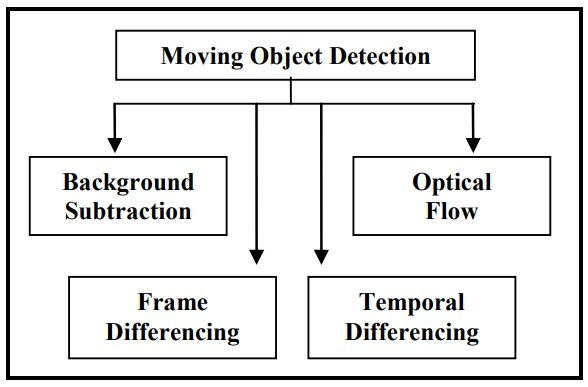
\includegraphics[width=8cm]{image/FourTraditionalMovingObjectDetection.jpg}
      \caption{Pendekatan Tradisional Deteksi Objek Bergerak}
      \small{Sumber: \citet{Kulchandani2015}}
      \label{fig:Pendekatan Tradisional Deteksi Objek Bergerak}
    \end{figure}
  
\section{\textit{Background Subtraction}}
    \textit{Background Subtraction} adalah metode yang digunakan untuk mendeteksi objek bergerak dalam video dengan cara membandingkan setiap \textit{frame} dengan sebuah \textit{(reference frame)} atau \textit{background model}, yang kemudian dihitung perbedaan nilai piksel diantara keduanya. Perbedaan inilah yang nantinya akan dikomparasi dengan sebuah \textit{threshold} yang nilainya sudah ditentukan. Jika perbedaan nilai piksel melebihi nilai \textit{threshold}, maka piksel tersebut dapat dikatakan bagian dari objek bergerak \textit{(foreground)} dan jika tidak, piksel akan dikatakan sebagai \textit{background} \citep{Desai2014}. Dalam banyak literasi, metode BS dapat dirumuskan sebagai berikut:
    \begin{equation}\label{eq:2.3}
    X_t (s) =
    \begin{cases} 
          1 &\text{\textit{if} $d(I_{s,t}, B_s) > T$}, \\
          0 &\text{\textit{otherwise}}
    \end{cases}
    \end{equation}
    
    Dimana $T$ adalah nilai \textit{threshold} yang sudah ditentukan, $X_t (s)$ adalah \textit{foreground mask} pada waktu $t$, $d$ adalah selisih antara $I_{s,t}$ yang merupakan nilai piksel $s$ pada waktu $t$, dengan $B_s$ yang merupakan \textit{background model} pada piksel $s$. Yang membedakan metode BS satu dengan yang lain biasanya terletak pada bagaimana metode tersebut memodelkan $B$ \citep{Benezeth2010}.
    
    \textit{Background modeling} adalah tahap yang penting dari \textit{Background Subtraction}. Objektif utama dari proses \textit{background modeling} adalah untuk mendapatkan model latar belakang yang berisikan informasi berupa bagian statis dari sebuah \textit{scene}, atau segala sesuatu yang dapat dikatakan sebagai latar belakang. Cara paling sederhana dalam memodelkan latar belakang $B$ adalah dengan sebuah citra yang berisikan \textit{scene} statis tanpa objek bergerak. Citra tersebut dapat diambil dari sebuah video ketika tidak ada objek yang bergerak di dalamnya.
    
    \vspace{0.5cm}
    \begin{figure}[H]
    \centering
      \singlespacing
      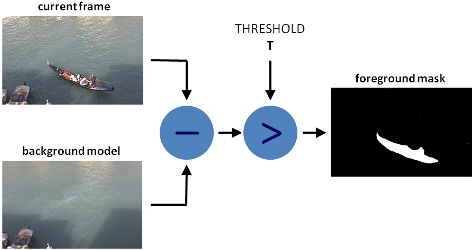
\includegraphics{image/BS.png}
      \caption{Skema sederhana metode \textit{Background Subtraction}}
      \small{Sumber: \href{https://docs.opencv.org/4.5.3/d1/dc5/tutorial_background_subtraction.html}{OpenCV - Background Subtraction}}
      \label{fig:BS}
    \end{figure}
    
    Dibalik kemudahan implementasinya, kelemahan dari metode tradisional ini adalah sistem tidak dapat mengatasi perubahan yang terjadi pada latar belakang selama video berlangsung. Karena dalam praktiknya, latar belakang sebuah video tidak akan selalu statis. Perubahan iluminasi, pergerakan berulang suatu objek (dahan pohon yang tertiup angin), atau perubahan bentuk geometri objek latar belakang tentu dapat memengaruhi akurasi metode ini.

\section{\textit{Background Subtraction} Menggunakan \textit{Gaussian Mixture Models}}
    \textit{Gaussian Mixture Models} (GMM) dapat digunakan untuk memodelkan latar belakang pada teknik \textit{Background Subtraction}. \citet{Stauffer1999}, dalam penelitiannya memodelkan sebuah piksel sebagai \textit{mixture of Gaussians}. Berdasarkan \textit{evidence} dan varians dari masing-masing distribusi Gaussian, dapat ditentukan distribusi mana yang masuk ke dalam kelas warna latar belakang \textit{(background color)}. Nilai piksel yang tidak masuk ke dalam distribusi warna latar belakang akan dianggap sebagai latar depan \textit{(foreground)} sampai ada distribusi Gaussian yang nilai piksel tersebut termasuk di dalamnya.
    
    Dikatakan oleh Stauffer bahwa sistem ini \textit{robust} terhadap latar belakang yang dinamis, seperti perubahan iluminasi, pergerakan berulang sebuah benda (dahan pohon yang tertiup angin), objek yang bergerak lambat, dan objek yang masuk serta keluar dari \textit{scene}. Objek yang bergerak lambat membutuhkan waktu yang lama untuk dapat dikatakan sebagai latar depan. Hal ini dikarenakan warna piksel mereka mempunyai varians yang lebih besar dibandingkan latar belakang. Sistem ini memiliki dua parameter, yaitu \textit{learning rate} $\alpha$ dan \textit{threshold} $T$ (proporsi data yang harus diperhitungkan/digunakan oleh latar belakang).
    
    \subsection{\textit{Gaussian Mixture Models}}
        Didefinisikan nilai sebuah piksel berturut-turut sebagai \textit{"pixel process"}. \textit{Pixel process} adalah serangkaian nilai piksel, nilai piksel tersebut dapat berupa skalar untuk citra \textit{grayscale} dan vektor untuk citra berwarna \textit{(r, g, b)}. Suatu hal yang dapat  diketahui dari sebuah piksel ${x_0, y_0}$ pada waktu $t$ adalah riwayat dari piksel itu sendiri.
        \begin{equation}\label{eq:2.4}
        \{X_1, \ldots, X_t\} = \{I(x_0, y_0, i) : 1 \leq i \leq t\}
        \end{equation}
        
        Dimana $I$ adalah serangkaian citra. Jika perubahan cahaya terjadi di dalam \textit{scene}, perubahan itu harus tetap dilacak oleh distribusi-distribusi Gaussian tersebut. Jika sebuah objek statis masuk ke dalam \textit{scene} dan tidak langsung masuk ke dalam distribusi latar belakang sampai objek tersebut sudah lebih lama ada di area tersebut dari objek sebelumnya, maka objek tersebut akan dikategorikan sebagai latar depan dalam waktu yang cukup lama. Hal ini akan berujung pada estimasi latar depan yang buruk. Misalnya dahan pohon yang bergerak karena tertiup angin, tentu tidak diinginkan objek tersebut dideteksi sebagai objek bergerak oleh sistem.
        
        Hal di atas adalah faktor yang menjadi landasan utama Stauffer dalam menentukan model dan prosedur updatenya. Riwayat dari setiap piksel $\{X_1, \ldots, X_t\}$ dimodelkan oleh $K$ distribusi Gaussian yang probabilitas nilai pikselnya didefinisikan oleh fungsi berikut
        
        \begin{equation}\label{eq:2.5}
        P(X_t) = \sum_{i=1}^K \omega_{i, t} \cdot \eta (X_t, \mu_{i, t}, \text{$\textstyle \sum$}_{i, t})
        \end{equation}
        
        Dimana $K$ adalah jumlah distribusi Gaussian, $\omega_{i, t}$ adalah estimasi dari \textit{evidence / weight / bobot} (proporsi data yang direpresentasikan oleh Gaussian yang bersangkutan), $\mu_{i, t}$ adalah nilai rata-rata dari Gaussian ke-$i$ pada waktu $t$, $\sum_{i, t}$ adalah kovarians matriks Gaussian ke-$i$ pada waktu $t$, dan $\eta$ adalah fungsi probabilitas Gaussian
        \begin{equation}\label{eq:2.6}
        \eta (X_t, \mu_t, \text{$\textstyle \sum$}) = 
        \frac{1}{{(2\pi)^\frac{n}{2} \textstyle |\sum|^\frac{1}{2} }}e^{ - \frac{1}{2} (X_t - \mu_t)^{T \sum{-1} } (X_t - \mu_t)}
        \end{equation}
        \vspace{0.005cm}
        
        Dengan kovarians matriks
        \begin{equation}\label{eq:2.7}
        \text{$\sum$}_{i, t} = \sigma^2_k I
        \end{equation}
        
        $K$ ditentukan oleh kemampuan komputasi komputer. Untuk nilai bawaan $K =  5$ diset dan dapat diatur sesuai dengan kebutuhan pengguna untuk mendapatkan hasil terbaik.
        
    \subsection{\textit{Modeling Process}}
        Distribusi intensitas untuk setiap nilai piksel dimodelkan oleh \textit{mixture of Gaussian}. Secara garis besar, jika ada nilai piksel baru yang masuk ke dalam model, piksel tersebut akan direpresentasikan oleh salah satu komponen atau distribusi Gaussian yang ada dan digunakan untuk memperbarui model tersebut. Teknik \textit{on-line K-means approximation} digunakan untuk memodelkan distribusi nilai masing-masing piksel.
        
        Langkah pertama yang harus dilakukan adalah, inisialisasi Gaussian $\eta$ untuk memodelkan nilai piksel pada observasi $X_1$ dengan $\omega = 1$, $\mu = X_1$, dan varians $\sigma$ yang besar. Observasi $X_1$ adalah observasi nilai sebuah piksel pada waktu $t$. Selanjutnya, setiap piksel baru $X_t$ diperiksa terhadap $K$ distribusi Gaussian yang sudah ada, sampai terdapat \textit{"match"}. Sebuah nilai piksel dapat dikatakan \textit{"match"} dengan $K$ distribusi Gaussian jika nilai piksel terletak dalam jangkauan 2,5 dari standar deviasi distribusi tersebut. Jika terdapat \textit{"match"}, parameter $(\omega, \mu, \sigma)$ dari distribusi Gaussian diperbarui sebagai berikut
        \begin{equation}\label{eq:2.8}
        \omega_{k, t} = (1 - \alpha)\omega_{k, t-1} + \omega(M_{k, t})
        \end{equation}
        \begin{equation}\label{eq:2.9}
        \mu_t = (1 - \rho)\mu_t-1 + \rho X_t
        \end{equation}
        \begin{equation}\label{eq:2.10}
        \sigma^2_t = (1 - \rho)\sigma^2_t-1 + \rho (X_t - \mu_t)^T (X_t - \mu_t)
        \end{equation}
        \vspace{0.005cm}
        
        Dimana $\alpha$ adalah \textit{learning rate}, $M_{k, t}$ bernilai 1 untuk distribusi yang \textit{"matched"}, dan 0 untuk distribusi yang lainnya. Lalu
        \begin{equation}\label{eq:2.11}
        \rho = \alpha\eta(X_t|\mu_t, \sigma_t)
        \end{equation}
        
        Jika tidak ada distribusi $K$ yang \textit{"match"} dengan nilai piksel baru tersebut, maka buat distribusi baru yang menggunakan nilai piksel baru sebagai rata-ratanya, nilai varians awal yang besar, dan juga bobot yang rendah. Distribusi yang paling kecil kemungkinannya akan digantikan oleh distribusi baru jika $K \text{\textit{Gaussians}} > K$.
        
    \subsection{\textit{Background Model Estimation}}
        Dalam tahap ini, ditentukan distribusi Gaussian mana yang merupakan bagian dari latar belakang. Secara heuristik, distribusi Gaussian yang memiliki bobot yang paling tinggi dan juga varians yang paling kecil adalah distribusi yang dapat diklasifikasikan sebagai latar belakang. Untuk memahami hal tersebut, diberikan sebuah objek statis yang mempunyai distribusi nilai piksel dengan bobot yang tinggi dan juga varians yang kecil. Objek statis ini dapat dikatakan sebagai \textit{background} dalam suatu \textit{scene} video. Ketika terdapat objek baru yang melewati objek statis tersebut, nilai piksel objek baru tidak akan \textit{"match"} dengan salah satu distribusi Gaussian yang sudah ada sebelumnya. Hal ini akan berujung pada pembuatan distribusi baru atau peningkatan nilai varians dari distribusi yang sudah ada. Selain itu, varians dari objek bergerak diasumsikan bernilai lebih besar daripada varians latar belakang. Untuk memodelkan hal tersebut, dibutuhkan sebuah metode yang dapat menentukan bagian mana dari model distribusi Gaussian yang secara akurat merepresentasikan latar belakang.
        
        Pertama, distribusi Gaussian diurutkan berdasarkan nilai $\omega/\sigma$ dari masing-masing distribusi. Kemudian, \textit{background model} dipilih berdasarkan fungsi berikut, dimana $T$ adalah sebuah ukuran untuk menentukan seberapa besar bagian dari data yang dapat diklasifikasikan sebagai latar belakang.
        \begin{equation}\label{eq:2.12}
        B = argmin_b (\sum_{k=1, b}\omega_k > T)
        \end{equation}
        
        
\section{Operasi Morfologi}
    Morfologi dalam konteks pengolahan citra adalah deskripsi bentuk dan struktur dari sebuah objek di dalam citra. Berdasarkan hal tersebut, operasi morfologi adalah sebuah operasi yang diaplikasikan terhadap bentuk dan struktur sebuah objek di dalam citra. Teknik ini bekerja berdasarkan teori himpunan. Operasi Morfologi mengambil input berupa citra biner ataupun citra \textit{grayscale} \citep{Srisha2013}. Operasi Morfologi dapat digunakan untuk memperbesar atau memperkecil ukuran objek. Operasi morfologi juga dapat digunakan untuk menutup ataupun membuka lubang pada sebuah objek dalam citra.
    
    Operasi morfologi melakukan "pemindaian" terhadap sebuah citra dengan menggunakan \textit{Structuring element}. \textit{Structuring element} adalah sebuah matriks biner yang biasanya direpresentasikan sebagai matriks persegi berdimensi ganjil. Mekanisme pemindaian citra menggunakan \textit{structuring element} sangat menyerupai \textit{kernel / mask} pada operasi konvolusi. Akan tetapi, alih-alih melakukan operasi konvolusi, \textit{structuring element} hanya melakukan operasi logika sederhana. Interaksi antara \textit{structuring element} dengan citra yang ingin diperiksa akan menghasilkan citra baru berdasarkan jenis operasi morfologi yang diterapkan pada citra tersebut.
    \begin{figure}[H]
    \centering
      \singlespacing
      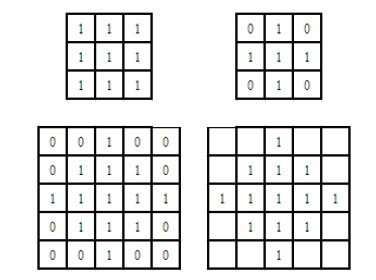
\includegraphics{image/StructuringElement.jpg}
      \caption{Representasi \textit{Structuring Element}}
      \small{Sumber: \citet{Srisha2013}}
      \label{fig:SS}
    \end{figure}
    
\section{Jenis - Jenis Operasi Morfologi}
    Walaupun operasi morfologi berdasar pada teori himpunan, banyak dari jenis operasi ini yang secara garis besar hanyalah operasi logika sederhana dan sangat mudah untuk digunakan. Terdapat dua jenis operasi fundamental dari operasi morfologi, yaitu erosi dan dilasi. Jenis operasi yang lain sangat bergantung kepada dua operasi fundamental tersebut.\\\\
    
    \subsection{Erosi}
        Operasi erosi membuat objek pada citra menjadi lebih kecil. Sederhananya, piksel di sekitar garis tepi sebuah objek akan dihilangkan. Erosi dapat digunakan untuk menghilangkan \textit{noise} pada citra dan juga memisahkan objek satu dengan yang lainnya. Erosi dari sebuah citra $A$ oleh \textit{structuring element} $B$ dapat didefinisikan oleh fungsi berikut
        \begin{equation}\label{eq:2.13}
        A \ominus B = \{z | (B)_z \subseteq A\}
        \end{equation}
        
        \textit{Structuring element} yang sudah dibuat akan memindai seluruh piksel di dalam citra dari mulai kiri ke kanan, dan dari atas ke bawah. Sebuah piksel tengah dari \textit{structuring element} akan dibiarkan bernilai 1 jika seluruh piksel di dalam \textit{structuring element} bernilai 1. Jika tidak, piksel akan dihilangkan atau diset nilainya menjadi 0 \textit{(background)}.
        \begin{figure}[H]
        \centering
          \singlespacing
          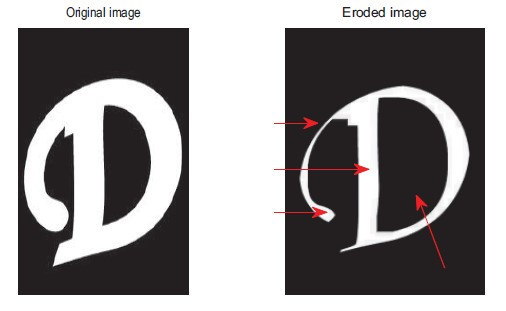
\includegraphics[width=10cm]{image/erosi.jpg}
          \caption{Operasi Erosi}
          \small{Sumber: \citet{Srisha2013}}
          \label{fig:Erosi}
        \end{figure}
    
    \subsection{Dilasi}
        Operasi dilasi membuat objek pada citra bertambah ukurannya menjadi lebih besar. Seberapa jauh operasi ini dapat membuat objek menjadi lebih besar bergantung pada bentuk dan ukuran \textit{structuring element}-nya. Dilasi sangat berguna untuk menutup lubang pada objek atau menggabungkan bagian-bagian objek yang terpisah. Operasi ini dapat didefinisikan sebagai
        \begin{equation}\label{eq:2.14}
        A \oplus B = \{z | \widehat{(B)_z} \cap A \neq \emptyset\}
        \end{equation}
        
        Sama seperti erosi, dilasi juga menggunakan \textit{structuring element} dalam proses pemindaian citra. Sebuah piksel tengah dari \textit{structuring element} diset nilainya menjadi 1 jika  \textit{structuring element} memiliki paling tidak satu piksel yang bernilai 1.
        \begin{figure}[H]
        \centering
          \singlespacing
          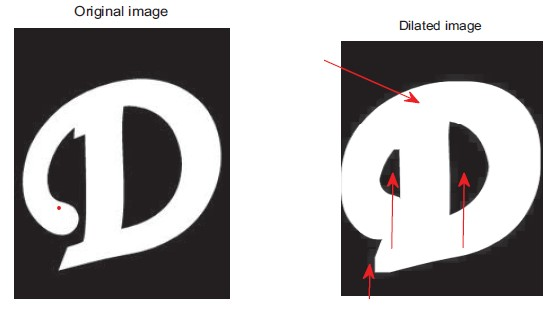
\includegraphics[width=12cm]{image/dilasi.jpg}
          \caption{Operasi Dilasi}
          \small{Sumber: \citet{Srisha2013}}
          \label{fig:Dilasi}
        \end{figure}
    
    \subsection{\textit{Opening}}
        \textit{Opening} adalah erosi yang diikuti oleh dilasi. Jenis operasi ini sangat berguna untuk menghilangkan objek yang sangat kecil atau \textit{noise} pada citra. \textit{Opening} citra $A$ oleh \textit{structuring element} $B$ dapat didefinisikan sebagai
        \begin{equation}\label{eq:2.15}
        A \text{ $o$ } B = (A \ominus B) \oplus B
        \end{equation}
        \begin{figure}[H]
        \centering
          \singlespacing
          
\includegraphics[width=8cm]{image/opening.jpg}
          \caption{Operasi \textit{Opening}}
          \small{Sumber: \href{https://docs.opencv.org/3.4.15/d3/dbe/tutorial_opening_closing_hats.html}{OpenCV - Opening}}
          \label{fig:Opening}
        \end{figure}
    
    \subsection{\textit{Closing}}
        \textit{Closing} adalah kebalikan dari operasi \textit{opening}. \textit{Closing} adalah dilasi yang diikuti oleh erosi. Seperti namanya, operasi \textit{closing} digunakan untuk menutup lubang di dalam sebuah objek atau menyambungkan bagian-bagian objek yang terpisah. \textit{Closing} citra $A$ oleh \textit{structuring element} $B$ dapat didefinisikan sebagai
        \begin{equation}\label{eq:2.16}
        A \text{ $o$ } B = (A \oplus B) \ominus B
        \end{equation}
        \begin{figure}[H]
        \centering
          \singlespacing
          
\includegraphics[width=8cm]{image/closing.jpg}
          \caption{Operasi \textit{Closing}}
          \small{Sumber: \href{https://docs.opencv.org/3.4.15/d3/dbe/tutorial_opening_closing_hats.html}{OpenCV - Closing}}
          \label{fig:Closing}
        \end{figure}

\section{\textit{Downsampling}}
    \textit{Downsampling} merupakan salah satu operasi fundamental yang sering digunakan dalam pengolahan citra. \textit{Downsampling} adalah proses mereduksi resolusi spasial dari sebuah citra dengan tetap mempertahankan representasi 2D dari citra tersebut. Operasi ini biasanya digunakan untuk mengurangi ukuran penyimpanan dari sebuah citra. Beberapa metode standar untuk melakukan operasi ini diantaranya adalah \textit{decimation} dan \textit{averaging}.

    \textit{Decimation} adalah proses mengeliminasi piksel dari sebuah citra. Terdapat beberapa \textit{pattern} yang biasa digunakan, seperti menghapus setiap baris dan kolom piksel yang bernomor genap. Metode lainnya adalah \textit{averaging}, yang menggabungkan beberapa piksel menjadi satu buah piksel dengan cara \textit{averaging} (dicari rata-ratanya).
    \begin{figure}[H]
    \centering
      \singlespacing
      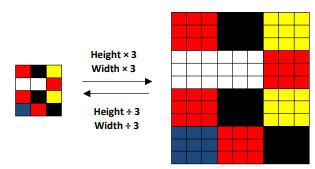
\includegraphics[width=7cm]{image/upsampling and downsampling.png}
      \caption{\textit{Image Downsampling dan Upsampling}}
      \small{Sumber: \citet{Paul2021}}
      \label{fig:Image Downsampling and Upsampling}
    \end{figure}
    \begin{figure}[H]
    \centering
      \singlespacing
      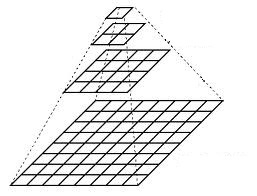
\includegraphics[width=5cm]{image/Pyramids_Tutorial_Pyramid_Theory.png}
      \caption{Piramid Citra}
      \small{Sumber: \href{https://docs.opencv.org/3.4/d4/d1f/tutorial_pyramids.html}{OpenCV - Image Pyramid}}
      \label{fig:Piramid Citra}
    \end{figure}

  
\section{Contour Tracing}
    \textit{Contour Tracing} atau \textit{Border Following} adalah salah satu teknik yang sangat penting dalam bidang pengolahan citra digital, terutama pada citra biner. \textit{Border following} telah dipelajari secara mendalam karena metode ini memiliki jangkauan pengaplikasian yang sangat luas, seperti pengenalan objek, analisis citra, deteksi objek, dan kompresi data citra \citep{Suzuki1985}.
    
    \citet{Suzuki1985} dalam penelitiannya menawarkan dua buah algoritme \textit{border following} yang sampai saat ini masih banyak digunakan oleh berbagai macam \textit{library} pengolahan citra modern seperti OpenCV. Algoritme ini adalah salah satu algoritme yang pertama kali mendefinisikan hubungan hierarki antar tepi \textit{(border)}. Selain itu, algoritme ini juga dapat membedakan tepi luar \textit{(outer border)} dan tepi lubang \textit{(hole border)} di sebuah objek. Beberapa definisi yang terdapat pada algoritme ini antara lain:
    
    \begin{itemize}
        \item \textbf{Definisi 1 (\textit{border point})}. Sebuah piksel bernilai 1 yang dikelilingi oleh piksel bernilai 0 dapat disebut sebagai \textit{border point}.
        \item \textbf{Definisi 2 (komponen yang mengelilingi komponen lain)}. Dari Gambar \ref{fig:Hubungan-antar-komponen-dan-tepi} dapat dikatakan bahwa komponen $S_2$ mengelilingi komponen $S_4$.
        \item \textbf{Definisi 3 (\textit{outer border} dan  \textit{hole border})}. Sebuah rangkaian \textit{border point} antara komponen yang mempunyai nilai piksel 1 (objek) dengan komponen yang mempunyai nilai piksel 0 (latar belakang).
        \item \textbf{Definisi 4 (\textit{parent border})}. Dari Gambar \ref{fig:Hubungan-antar-komponen-dan-tepi} dapat dikatakan bahwa tepi $B_2$ adalah \textit{parent border} dari tepi $B_3$.
        \item \textbf{Definisi 5 (tepian yang mengelilingi tepian lain)}. Dari Gambar \ref{fig:Hubungan-antar-komponen-dan-tepi} dapat dikatakan bahwa tepi $B_2$ mengelilingi tepi $B_3$.
    \end{itemize}
    \begin{figure}[H]
    \centering
      \singlespacing
      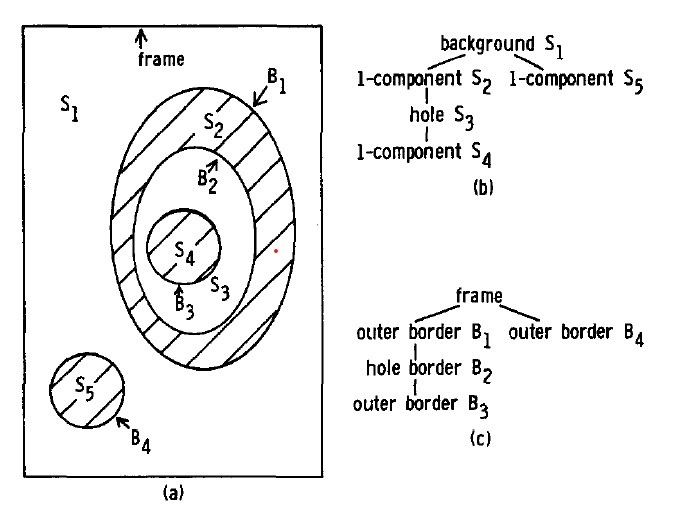
\includegraphics[width=10cm]{image/surroundess.jpg}
      \caption{Hubungan antar komponen dan tepi}
      \small{Sumber: \citep{Suzuki1985}}
      \label{fig:Hubungan-antar-komponen-dan-tepi}
    \end{figure}
    
    Diasumsikan citra masukan algoritme ini berupa citra biner. Piksel dengan nilai 0 dan 1 disebut sebagai 0-piksel dan 1-piksel. Piksel bernilai 0 merepresentasikan latar belakang, sementara piksel bernilai 1 merepresentasikan latar depan (objek). Didefinisikan $f_{i, j}$ sebagai nilai sebuah piksel pada koordinat $(i, j)$ yang masing-masing melambangkan baris dan kolom sebuah citra digital. Baris paling atas, baris paling bawah, kolom paling kiri, dan kolom paling kanan adalah \textit{frame} dari citra tersebut. Dalam hal ini, diberikan angka unik untuk setiap tepi baru yang ditemukan dan bisa disebut sebagai \textbf{NBD}. Asumsikan NBD dari \textit{frame} adalah 1, sementara tepi lain diberikan angka NBD secara berurutan. Nilai NBD dari \textit{parent} setiap tepi di dalam variabel \textbf{LNBD} kemudian disimpan. Berikut adalah langkah-langkah \textit{border following} algoritme 1:
    
    Mulai memindai piksel citra dari kiri ke kanan hingga \textit{scanner} menemukan piksel objek $f_{i, j} \neq 0$. Lalu tentukan apakah piksel tersebut merupakan tepi luar atau tepi lubang. Untuk setiap baris baru yang dipindai, \textit{reset} $LNBD$ ke 1.\\\\
    
    \begin{enumerate}
        \item Langkah 1
        
        \begin{enumerate}[label=(\alph*)]
            \item Jika $f_{i, j} = 1$ dan $f_{i, j - 1} = 0$, maka piksel $(i, j)$ adalah \textit{starting point} dari operasi \textit{border following} untuk tepi luar \textit{(outer border)}. Inkremen $NBD$ dan set $(i_2, j_2) \leftarrow (i, j-1)$.
            \item Jika $f_{i, j} \geq 1$ dan $f_{i, j+} = 0$, maka piksel $(i, j)$ adalah \textit{starting point} dari operasi \textit{border following} untuk tepi lubang \textit{(hole border)}. Inkremen $NBD$, set $(i_2, j_2) \leftarrow (i, j + 1)$, dan $LNBD \leftarrow f_{i, j}$ jika $f_{i, j} > 1$.
            \item Jika dua kondisi di atas tidak terpenuhi, maka lanjutkan ke langkah 4.
        \end{enumerate}
        
        \vspace{-0.9cm}
        \begin{figure}[H]
        \centering
          \singlespacing
          \captionsetup{justification=centering,margin=2cm}
          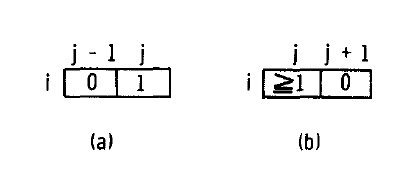
\includegraphics[width=6cm]{image/outerorholeborder.jpg}
          \caption{Kondisi \textit{starting point} dari algoritme \textit{border following} untuk tepi luar (a) dan tepi lubang (b)}
          \small{Sumber: \citep{Suzuki1985}}
          \label{fig:outerandholeborder}
        \end{figure}
        
        \item Langkah 2
        
        Berdasarkan jenis tepi dari piksel $(i, j)$ dan jenis tepi dari $LNBD$ (tepi terakhir yang ditemukan), dapat ditentukan \textit{parent border} untuk tepi piksel $(i, j)$ seperti yang terlihat pada Tabel \ref{tab:parentborder}.
    
    	\vspace{3cm}
	    \begin{longtblr}[
	    	caption = {Aturan penetapan \textit{parent border}},
	    	label = {tab:parentborder}
	    	]{
	    		colspec={|c|Q[c,m,4.5cm]|Q[c,m,4.5cm]|},
	    		rowhead=1
	    	}
	    	\hline
	    	& \SetCell[c=2]{} \textit{Type of the border B' with the sequential number LNBD} \\ \hline
	    	\textit{Type of B} & \textit{Outer border} & \textit{Hole border} \\ \hline
	    	\textit{Outer border} & \textit{The parent border of the border B'} & \textit{The border B'} \\ 
	    	\textit{Hole border} & \textit{The border B'} & \textit{The parent border of the border B'} \\ 
	    	\hline
	    \end{longtblr}
        
        \item Langkah 3
        
        Pada langkah ini, dimulai dari \textit{starting point} piksel $(i, j)$ lakukan proses \textit{border following}:
        \begin{enumerate}
            \item Dimulai dari piksel $(i_2, j_2)$, searah jarum jam periksa piksel tetangga dari piksel $(i, j)$ sampai menemukan piksel \textit{non-zero}. Didefinisikan piksel \textit{non-zero} yang pertama ditemukan sebagai $(i_1, j_1)$. Jika piksel \textit{non-zero} tidak ditemukan, set $f_{i, j} = -NBD$ dan lanjutkan ke langkah 4.
            
            \item $(i_2, j_2) \leftarrow (i_1, j_1)$ dan $(i_3, j_3) \leftarrow (i, j)$.
            
            \item Mulai dari elemen selanjutnya dari piksel $(i_2, j_2)$, berlawanan arah jarum jam carilah piksel \textit{non-zero} di sekitar piksel $(i_3, j_3)$ dan set piksel $non-zero$ pertama yang ditemukan tersebut ke dalam variabel $(i_4, j_4)$.
            
            \item Ubah nilai $f_{i_3, j_3}$ dari piksel $(i_3, j_3)$ seperti berikut \textit{marking policy}:
            \begin{enumerate}
                \item Jika piksel $(i_3, j_3 + 1)$ dari langkah (3.a) adalah 0-piksel (piksel bernilai 0), set $(i_3, j_3 + 1) \leftarrow -NBD$
                \item Jika piksel $(i_3, j_3 + 1)$ dari langkah (3.a) bukan 0-piksel (piksel bernilai 0), set $(i_3, j_3 + 1) \leftarrow NBD$
                \item Jika kedua kondisi di atas tidak terpenuhi, jangan ubah nilai  $f_{i_3, j_3}$
            \end{enumerate}
            
            \item Jika  $(i_4, j_4) = (i, j)$ dan $(i_3, j_3) = (i_1, j_1)$ (kembali ke \textit{starting point}), maka lanjut ke langkah 4, Jika tidak set $(i_2, j_2) \leftarrow (i_3, j_3)$, $(i_3, j_3) \leftarrow (i_4, j_4)$ dan kembali ke langkah (3.a).
        \end{enumerate}
        
        \item Langkah 4
        
        Jika $f_{i, j} \neq 1$, maka $LNBD \leftarrow |f_{i, j}|$ dan lanjutkan pemindaian dari mulai piksel $(i, j+1)$ untuk kembali mencari nilai piksel objek $f_{i, j} \neq 0$. Alrogritme dinyatakan selesai jika \textit{scanner} sudah sampai sudut kanan bawah dari citra  tersebut (piksel terakhir).
        
        \begin{figure}[H]
        \centering
          \singlespacing
          \captionsetup{justification=centering,margin=0.5cm}
          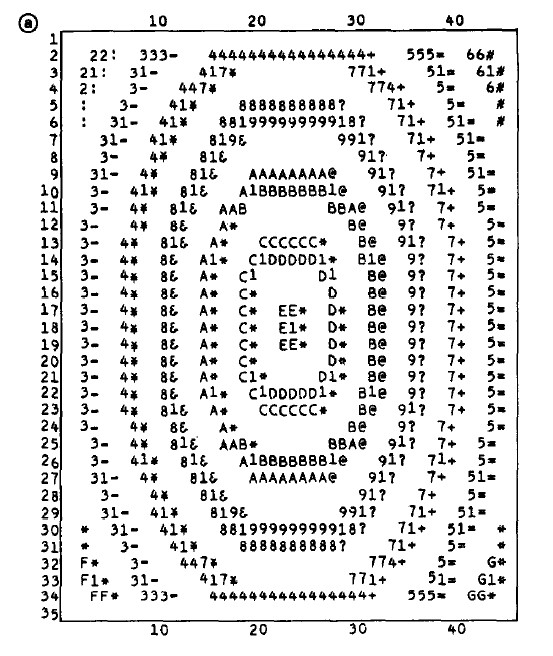
\includegraphics[width=8cm]{image/topologicalresult.jpg}
          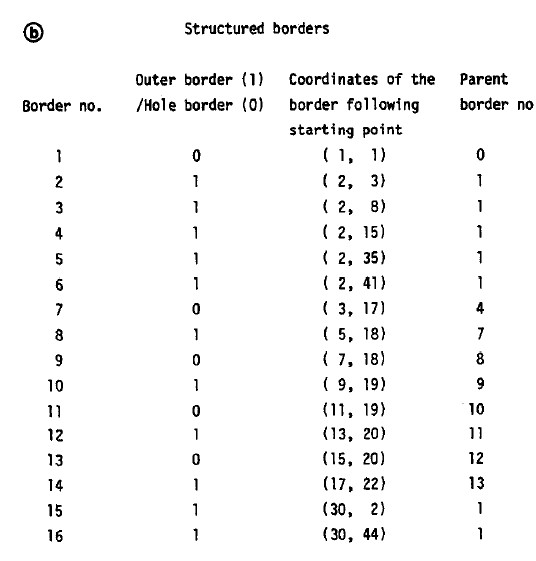
\includegraphics[width=10cm]{image/topologicalstructure.jpg}
          \caption{Struktur topologi antara tepi satu dengan tepi yang lain jika menggunakan Algoritme 1. Hasil citra (a) dan Struktur yang diekstrak (b)}
          \small{Sumber: \citep{Suzuki1985}}
          \label{fig:parentborder}
        \end{figure}
    \end{enumerate}
    
    Selain algoritme di atas, Suzuki juga mengusulkan algoritme \textit{border following} yang hanya akan menghasilkan tepi terluarnya saja. Beberapa perbedaan algoritme 1 dan algoritme 2 antara lain adalah:
    
    \begin{enumerate}
        \item Kondisi \textit{starting point} untuk melakukan operasi \textit{border following} hanya berlaku untuk tepi terluar (Gambar \ref{fig:outerandholeborder}) dan jika $LNBD \leq 0$.
        \item \textit{Marking policy} tetap sama dengan algoritme 1 (Langkah 3.d), tetapi nilai dari $NBD$ dan $-NBD$ akan digantikan masing-masing oleh nilai $2$ dan  $-2$.
        \item Nilai $LNBD$ juga tetap disimpan dari piksel \textit{non-zero} yang ditemukan sebelumnya. Akan tetapi, $LNBD$ akan di reset ke nilai 0 untuk setiap baris baru yang dipindai.
    \end{enumerate}
    \vspace{-0.9cm}
    \begin{figure}[H]
    \centering
      \singlespacing
      \captionsetup{justification=centering,margin=0.5cm}
      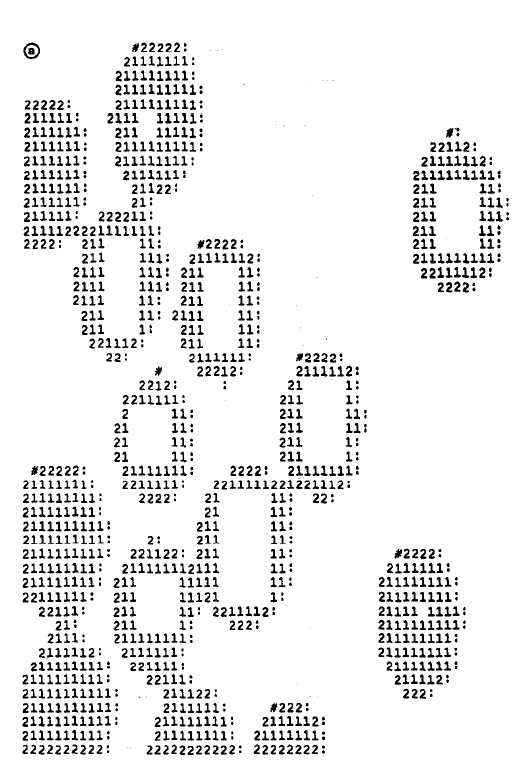
\includegraphics[width=8.1cm]{image/algoritma2.jpg}
      \caption{Hasil dari algoritme 2. Tanda "\#" merepresentasikan \textit{starting point} dan ":" merepresentasikan nilai $-2$}
      \small{Sumber: \citep{Suzuki1985}}
      \label{fig:parentborder}
    \end{figure}
    
\section{Pelacakan Objek}
    Pelacakan objek \textit{(object tracking)} mengacu kepada penggunaan sensor untuk menentukan lokasi, lintasan, atau bahkan karakteristik dari sebuah objek. Dalam kasus video, pelacakan objek didefinisikan sebagai sebuah tindakan melakukan estimasi atau prediksi terhadap lintasan sebuah objek bergerak di setiap \textit{frame} dalam video. Dengan kata lain, sebuah \textit{tracker} dapat memberikan label / identitas yang konsisten terhadap objek yang dilacak selama video berlangsung. Selain itu, sebuah \textit{tracker} juga dapat memberikan informasi lain yang berkaitan dengan objek tersebut, seperti orientasi, ukuran, atau bentuk geometrinya \citep{Yilmaz2006}.
    
    Permintaan terhadap teknologi analisis video yang lebih \textit{advanced} membuat metode pelacakan objek menjadi sangat menarik untuk dikembangkan. Penggunaan metode pelacakan objek sangat berguna dalam berbagai bidang, antara lain seperti \textit{motion recognition}, pengawasan, pemantauan lalu lintas, navigasi kendaraan, dan masih banyak lagi. Pelacakan objek merupakan dasar teori dari metode penghitungan objek \textit{(objek counting)}.
  
\section{Kalman Filter}

    \subsection{Definisi}
        Secara matematis, Kalman Filter adalah sebuah algoritme \textit{estimator} yang dapat melakukan prediksi dan koreksi terhadap keadaan sebuah proses linear \citep{Chavan2017}. Model matematis yang akurat sangat diperlukan untuk mendapatkan hasil yang optimal. Kalman Filter memiliki bentuk yang relatif sederhana dan tidak membutuhkan kekuatan komputasi yang besar.
        
        Kalman filter digunakan untuk melakukan estimasi suatu keadaan $x$ dalam sistem linear. Model dari proses \textit{(process model)} yang mendefinisikan evolusi suatu keadaan dari waktu $k - 1$ sampai waktu $k$ adalah:
        \begin{equation}\label{eq:2.17}
        x_k = Fx_{k-1} + Bu_{k-1} + w_{k-1} 
        \end{equation}
        
        dimana $F$ adalah matriks transisi dari keadaan $x$ yang diterapkan pada vektor keadaan sebelumnya $x_{k-1}$, $B$ adalah matriks kontrol yang diterapkan pada vektor kontrol $u_{k-1}$, dan $w_{k-1}$ adalah vektor proses \textit{noise} yang diasumsikan sebagai Gaussian dengan rata-rata nol dan kovarians $Q$, i.e., $w_{k-1} \sim N(0, Q)$.
        
        Model proses di atas dipasangkan dengan model pengukuran / observasi \textit{(measurement / observation model)} yang menggambarkan hubungan antara keadaan dan observasi pada waktu $k$ sebagai:
        \begin{equation}\label{eq:2.18}
        z_k = Hx_{k} + v_{k} 
        \end{equation}
        
        dimana $z_k$ adalah vektor observasinya, H adalah matriks transisi dari observasi $z$, dan $v_{k}$ adalah vektor \textit{noise} dari observasi yang diasumsikan sebagai Gaussian dengan rata-rata nol dan kovarians $R$, i.e., $v_{k} \sim N(0, R)$.
        
        Peran dari Kalman Filter adalah untuk memberikan estimasi $x$ pada waktu $k$, mengingat diberikannya estimasi awal $x_0$, rangkaian observasi $z1, z1, ..., zk$, dan informasi sistem yang digambarkan oleh $F$, $B$, $H$, $Q$, dan $R$. Walaupun matriks kovarians ($Q$ dan $R$) seharusnya mencerminkan statistik dari \textit{noise} masing-masing model, dalam banyak pengaplikasiannya di dunia nyata, model statistika dari \textit{noise} tersebut tidak benar-benar dapat dimodelkan. Karena hal itu, $Q$ dan $R$ biasanya digunakan sebagai \textit{tuning parameter} yang bisa digunakan untuk mendapatkan hasil dan performa yang diinginkan.
    
    \subsection{Algoritme Kalman Filter}
        Kalman Filter terdiri dari dua tahap, yaitu \textit{predict} dan \textit{update}. Dalam literasi lain, tahapan ini juga biasa disebut sebagai \textit{propagation} dan \textit{correction}. Tahapan \textit{predict} dan \textit{update} dapat diringkas ke dalam persamaan berikut:\\\\
        
        \noindent\textit{Predict}
        \begin{equation}\label{eq:2.19}
        \hat{x}^-_k = F\hat{x}^+_{k-1} + Bu_{k-1}
        \end{equation}
        \begin{equation}\label{eq:2.20}
        P^-_k = FP^+_{k-1}F^T + Q
        \end{equation}
        \textit{Update}
        \begin{equation}\label{eq:2.21}
        \tilde{y}_k = z_k - H\hat{x}^-_k
        \end{equation}
        \begin{equation}\label{eq:2.22}
        K_k = P^-_kH^T(R + HP^-_kH^T)^{-1}
        \end{equation}
        \begin{equation}\label{eq:2.23}
        \hat{x}^+_k = \hat{x}^-_k + K_k\tilde{y}
        \end{equation}
        \begin{equation}\label{eq:2.24}
        P^+_k = (I - K_kH)P^-_k
        \end{equation}
        
        Dari persamaan di atas, operator hat ($\string^$) menandakan sebuah estimasi dari sebuah variabel. Dengan kata lain, $\hat{x}$ adalah estimasi dari $x$. Superskrip $-$ dan $+$ masing-masing menyatakan estimasi yang diprediksi \textit{(prior)} dan diperbarui \textit{(posterior)}.
        
        Untuk memprediksi estimasi dari sebuah keadaan $\hat{x}^-_k$ dibutuhkan estimasi keadaan $\hat{x}^+_{k-1}$ dari iterasi Kalman Filter sebelumnya. Variabel $P$ adalah matriks kovarians dari keadaan $x$. Matriks kovarians ini digunakan untuk membantu Kalman Gain $K_k$ dalam menentukan bobot terhadap nilai yang diprediksi atau nilai yang diukur.
        
        Dalam tahap \textit{update}, $K_k$ pada Persamaan \ref{eq:2.22} adalah Kalman Gain. Nilai dari Kalman Gain akan berada diantara 0 dan 1. Kemudian nilai tersebut digunakan untuk memperbarui estimasi keadaan $\hat{x}^+_k$. Jika nilai dari Kalman Gain mendekati 1, maka observasi dikatakan akurat dan estimasi dikatakan tidak akurat (\textit{error} besar). Begitu juga sebaliknya, jika $K_k$ mendekati 0, maka observasi dikatakan tidak akurat dan estimasi dapat dikatakan akurat (\textit{error} kecil). Akibatnya, nilai $K_k$ yang kecil akan membuat selisih antara keadaan yang diobservasi dan keadaan yang diestimasi mempunyai efek yang kecil terhadap proses pembaruan keadaan (Persamaan \ref{eq:2.23}). Residual pengukuran $\tilde{y}_k$ adalah selisih antara nilai yang diobservasi $z_k$, dengan nilai yang diestimasi $H\hat{x}^-_k$. Residual pengukuran $\tilde{y}_k$ kemudian dikalikan dengan Kalman Gain $K_k$ untuk memberikan koreksi $K_k\tilde{y}_k$ terhadap estimasi keadaan $\hat{x}^-_k$ (Persamaan \ref{eq:2.23}). Setelah mendapatkan estimasi keadaan yang baru, Kalman Filter menghitung kovarians $P^+_k$ untuk kemudian digunakan pada tahap atau iterasi Kalman Filter selanjutnya. Dapat dilihat bahwa kovarians $P^+_k$ mempunyai nilai yang lebih kecil dibandingkan kovarians $P^-_k$, yang berarti Kalman Filter menjadi lebih yakin dengan estimasi keadaan setelah tahap \textit{update}.
        
        Dibutuhkan tahap inisialisasi untuk dapat mengimplementasi Kalman Filter. Dalam tahap tersebut, dibutuhkan tebakan awal dari $\hat{x}^+_0$ dan juga matriks kovarians $P^+_0$. Bersama dengan $Q$ dan $R$, $\hat{x}^+_0$ dan $P^+_0$ memainkan peran yang sangat penting untuk mendapatkan hasil dan performa yang diinginkan. Sebagai \textit{"rule of thumb"}, kovarians $P^+_0$ dapat diset ke nilai yang besar untuk konvergensi yang lebih cepat. Secara keseluruhan, Kalman Filter dapat diimplementasi dengan menerapkan tahap \textit{predict} dan tahap \textit{update} untuk setiap iterasi waktu $k = 1, 2, 3, ...$ setelah tahap inisialisasi dilakukan.
        
        Perlu dicatat bahwa Kalman Filter bekerja berdasarkan asumsi bahwa model proses \textit{(process model)} dan model pengukuran \textit{(measurement model)} merupakan model yang linear, yang berarti model-model tersebut dapat diekspresikan dengan matriks F, B, dan H. Oleh karena itu, Kalman Filter dapat memberikan hasil estimasi yang optimal jika dan hanya jika asumsi di atas terpenuhi.
        
\section{\textit{Decision of Occlusion}}
    \textit{Occlusion} adalah sebuah peristiwa dimana dua atau lebih objek saling bertumpuk satu sama lain. Hal ini tentu dapat berpengaruh terhadap performa sistem jika tidak ditangani dengan baik. \textit{Occlusion} pada dasarnya mencakup dua masalah, yaitu masalah \textit{merge} dan \textit{split}. Menyatunya dua atau lebih objek disebut sebagai proses \textit{merge}. Sebaliknya, terpisahnya objek yang sebelumnya menyatu disebut sebagai proses \textit{split}. Proses \textit{merge} dan \textit{split} diilustrasikan pada Gambar \ref{fig:mergesplit}.
    \begin{figure}[H]
    \centering
      \singlespacing
      \captionsetup{justification=centering,margin=0.5cm}
      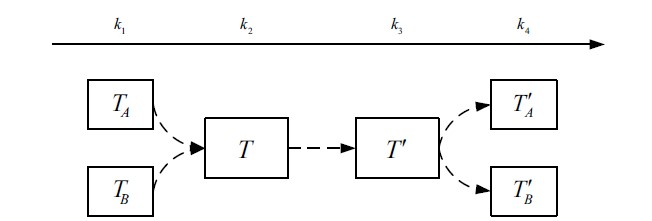
\includegraphics[width=12cm]{image/mergesplit-02.jpg}
      \caption{Ilustrasi dari proses \textit{merge} dan \textit{split}}
      \small{Sumber: \citep{Li2010}}
      \label{fig:mergesplit}
    \end{figure}
    
    Ketika dua atau lebih keadaan objek yang diprediksi menggunakan Kalman Filter mempunyai pasangan observasi (deteksi) yang sama, maka akan terjadi proses \textit{merge} sebagai bagian dari salah satu proses \textit{decision of occlusion}. Dua buah objek $T_A$ dan $T_B$ mengalami proses \textit{merge} pada waktu $k_1$. Dimulai dari waktu $k_2$, objek $T$ akan dilacak sebagai objek baru, Kalman Filter diinisialisasi untuk objek tersebut. Selama waktu $k_2$ sampai $k_3$, objek $T$ akan terus diupdate bersamaan dengan objek $T_A$ dan objek $T_B$. Objek $T$ kini menjadi objek $T'$. Pada waktu $k_4$, terjadi proses \textit{split} terhadap objek $T'$ menjadi objek $T'_A$ dan $T'_B$. Kedua objek tersebut kemudian dipasangkan kembali dengan objek $T_A$ dan $T_B$, membuat objek $T'$ hasil dari proses \textit{merge} sebelumnya kehilangan pasangan observasinya. Jika selama $k_n$ objek $T'$ terus menerus kehilangan pasangan observasinya, maka objek $T'$ akan dihapus.
    
    

\section{Asosiasi Data}
    Pada proses asosiasi data, prediksi estimasi keadaan dari sebuah objek yang dihasilkan oleh Kalman Filter kemudian diasosiasikan dengan observasi keadaan objek pada \textit{frame} selanjutnya, agar identitas dari objek tersebut dapat dipertahankan selama video berlangsung. Penelitian ini berfokus kepada pelacakan lebih dari satu objek. Dalam lingkungan yang mempunyai banyak objek,  bisa didapatkan hasil pelacakan lebih dari satu objek. Setiap objek ikan dalam video dideskripsikan oleh \textit{bounding box} dan titik pusatnya masing-masing. Untuk mendapatkan hasil pelacakan objek yang akurat, proses asosiasi data perlu dilakukan dengan menggunakan jarak antara keadaan objek yang diestimasi dengan hasil observasi serta luas dari objek tersebut sebagai \textit{cost function}. Secara garis besar, \textit{cost function} ini digunakan untuk mengklasifikasikan objek hasil dari prediksi Kalman Filter dengan objek hasil dari observasi (deteksi). Pertama, jarak antara dua titik pusat didefinisikan sebagai: 
    \begin{equation}\label{eq:3.5}
    D_k(i, j) = \frac{|\sqrt{(p_{k-1}^j - p_{k}^i)^2 + (q_{k-1}^j - q_{k}^i)^2}|}{max|(p_{k-1}^j - p_{k}^i)^2 + (q_{k-1}^j - q_{k}^i)^2|}
    \end{equation}
    
    dimana $p_{k-1}^j$ dan $q_{k-1}^j$ adalah nilai titik pusat dari koordinat $x$ dan $y$ yang didapatkan dari keadaan $\hat{x}_{k-1}^+$ dalam iterasi ke $j^{th}$. Lalu $p_{k}^i$ dan $q_{k}^i$ adalah nilai titik pusat dari koordinat $x$ dan $y$ yang didapatkan dari observasi $z_k$ dalam iterasi ke $i^{th}$. Variabel $i = 1, ..., m$ dan $j = 1, ..., n$ dimana $m$ adalah jumlah objek yang terdeteksi dari hasil observasi pada \textit{frame} $k$ dan $n$ adalah jumlah objek yang dihasilkan oleh estimasi Kalman Filter pada \textit{frame} $k-1$. Kedua, luas antara dua objek didefinisikan sebagai:
    \begin{equation}\label{eq:3.6}
    A_k(i, j) = \frac{|A_{k}^i - A_{k-1}^j|}{max|A_{k}^i - A_{k-1}^j|}
    \end{equation}
    
    Dimana $A_{k}^i = 4 l_k^i h_k^i$ dan $A_{k-1}^j = 4 l_{k-1}^j h_{k-1}^j$ yang merepresentasikan \textit{bounding box}. Semakin kecil nilai fungsi di atas, semakin mirip deskripsi bentuk dari dua objek tersebut. Dengan mengombinasikan persamaan \ref{eq:3.5} dan persamaan \ref{eq:3.6}, didefinisikan \textit{cost function} sebagai berikut. 
    \begin{equation}\label{eq:3.7}
    C_k(i, j) = \alpha D_k(i, j) + \beta A_k(i, j)
    \end{equation}
    
    Dimana $\alpha + \beta = 1$, parameter ini dapat diatur secara eksperimental, dalam hal ini digunakan $\alpha = 0.8$ dan $\beta = 0.2$. Variabel $\alpha$ dan $\beta$ menitik beratkan \textit{cost function} mana yang akan lebih besar digunakan nilainya. Tidak ada aturan khusus dalam menentukan $\alpha$ dan $\beta$. Semakin besar nilai $\alpha$ maka sistem akan semakin bias terhadap \textit{cost function} jarak objek. Sebaliknya, semakin besar nilai $\beta$, maka sistem akan semakin bias terhadap \textit{cost function} luas objek. Jika hasil dari \textit{cost function} di atas bernilai kecil, dapat diasumsikan bahwa dua objek tersebut memiliki korespondensi.
    

% Baris ini digunakan untuk membantu dalam melakukan sitasi
% Karena diapit dengan comment, maka baris ini akan diabaikan
% oleh compiler LaTeX.
\begin{comment}
\bibliography{collection}
\end{comment}


%!TEX root = ./template-skripsi.tex
%-------------------------------------------------------------------------------
%                            BAB III
%               		METODE PENELITIAN
%-------------------------------------------------------------------------------

\chapter{METODE PENELITIAN}

\section{Deskripsi Sistem}
    Sistem yang akan dibuat pada penelitian ini adalah sistem yang dapat melakukan pelacakan pergerakan objek ikan dengan menggunakan metode GMM dan Kalman Filter. Fokus dari penelitian ini adalah untuk menghasilkan \textit{output} berupa video yang di dalamnya terdapat objek yang sudah dilacak lengkap dengan \textit{bounding box} serta label uniknya. Dataset video yang akan digunakan pada sistem ini berasal dari dua sumber. Sementara bahasa pemrograman yang digunakan untuk membuat sistem adalah Python versi 3. 
    
    Tahapan proses pelacakan pergerakan objek ikan dengan menggunakan metode GMM dan Kalman Filter adalah memasukan \textit{input} video, deteksi objek bergerak dengan GMM, \textit{noise removal} dengan \textit{Morphology Operation}, \textit{Contour Tracing}, \textit{tracking} masing-masing objek menggunakan Kalman Filter, \textit{decision of occlusion}, dan terakhir adalah tahap asosiasi data. Tahapan-tahapan tersebut akan terus berulang selama video berlangsung.
    
\section{Perancangan Sistem}
    Bagian ini membahas tentang desain proses yang digunakan untuk mengetahui tahapan-tahapan yang dilakukan untuk membangun sistem pelacakan pergerakan objek ikan. Tahapan tersebut adalah sebagai berikut: tahap \textit{input} video yang kemudian dibaca oleh sistem dalam bentuk citra (\textit{frame} per \textit{frame}). Lalu dilakukan proses deteksi objek ikan yang bergerak menggunakan GMM, setelah itu dilakukan proses \textit{Morphology Operation} untuk menghilangkan \textit{noise} dari proses deteksi objek menggunakan GMM. Kemudian teknik \textit{downsampling} dan \textit{contour tracing} dijalankan untuk menghasilkan \textit{border} dari piksel yang dapat dikatakan sebagai objek. \textit{Bounding box} kemudian dipasangkan kepada masing-masing objek tersebut dan \textit{decision of occlusion} dilakukan. Terakhir Kalman Filter diinisiasi atau diperbarui untuk setiap objek yang ada. Hal ini dilakukan untuk memasangkan atau mempertahankan label unik masing-masing objek sehingga objek dapat terus dilacak atau diasosiasikan dengan tepat selama video berlangsung. Keluaran yang dihasilkan adalah sebuah \textit{running} video yang di dalamnya terdapat objek-objek yang sudah dilacak lengkap dengan label unik serta \textit{bounding box}-nya.
    \begin{figure}[H]
    \centering
      \singlespacing
      \captionsetup{justification=centering,margin=0.5cm}
      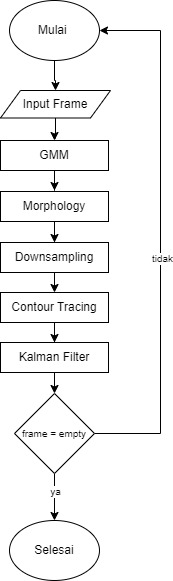
\includegraphics[width=4cm]{image/system-flow-chart.jpg}
      \caption{Diagram alir keseluruhan proses sistem}
      \label{fig:overalfc}
    \end{figure}
    
    \subsection{Proses Input Video}
        Data yang digunakan sebagai masukan dari sistem adalah video dengan format .mp4 atau .flv. Masukan video dibaca ke dalam bentuk citra sehingga menghasilkan \textit{frame} video. Setiap \textit{frame} video juga melalui proses \textit{pre-processing} dahulu sebelum masuk ke tahap deteksi objek dengan metode GMM yaitu, mengubah ruang warna citra dari RGB ke \textit{grayscale} .
        
    \subsection{Keluaran}
        Keluaran yang diharapkan dari sistem  adalah \textit{running} video yang di dalamnya sudah terdapat objek yang dilacak menggunakan metode GMM dan Kalman Filter lengkap dengan \textit{bounding box} serta label unik yang mengikutinya.
        
    \subsection{Deteksi Objek dengan GMM}
        Metode yang digunakan untuk mendeteksi objek ikan bergerak pada video adalah \textit{Background Subtraction} dengan bantuan GMM untuk memodelkan latar belakangnya. Langkah pertama pada GMM adalah inisialisasi Gaussian $\eta$ untuk memodelkan nilai piksel pada observasi $X_1$ dengan $\omega = 1$, $\mu = X_1$, dan varians $\sigma$. Observasi $X_1$ adalah observasi nilai sebuah piksel pada waktu $t$.
        
        Selanjutnya, setiap piksel baru $X_t$ akan diperiksa terhadap $K$ distribusi Gaussian yang sudah ada sampai terdapat \textit{"match"}. Sebuah piksel dapat dikatakan \textit{"match"} jika nilai piksel tersebut terletak dalam jangkauan 2,5 dari nilai standar deviasi sebuah distribusi. Jika terdapat \textit{"match"} maka parameter $(\omega, \mu, \sigma)$ dari distribusi Gaussian tersebut diperbaharui. \textit{Learning rate} $\alpha$ merupakan parameter dari sistem. Jika tidak terdapat \textit{"match"}, maka distribusi lama yang mempunyai nilai kemungkinan paling kecil akan digantikan oleh distribusi baru. Distribusi  baru  ini  menggunakan  nilai  piksel  baru  sebagai  rata-rataanya, memiliki nilai varians awal yang besar, dan juga bobot yang rendah.\\
        
        Distribusi $K$ kemudian diurutkan berdasarkan nilai $\omega/\sigma$ dari masing-masing distribusi dan distribusi $B$ pertama dijadikan sebagai model dari latar belakang. Penentuan distribusi $B$ pertama sebagai model latar belakang ditentukan oleh parameter $T$. \textit{Threshold} $T$ adalah sebuah nilai minimum yang digunakan untuk menentukan distribusi $B$ mana yang dapat dikatakan sebagai latar belakang. Untuk setiap distribusi $B$ yang tidak masuk ke dalam klasifikasi latar belakang dapat dikatakan sebagai latar depan (objek bergerak). Keluaran dari proses ini adalah citra biner dengan nilai $0$ sebagai latar belakang dan nilai $1$ sebagai latar depannya. Alur diagram proses \textit{Background Subtraction} dengan bantuan GMM dapat dilihat pada Gambar \ref{fig:gmmflowchart}.
        \begin{figure}[H]
        \centering
          \singlespacing
          \captionsetup{justification=centering,margin=0.5cm}
          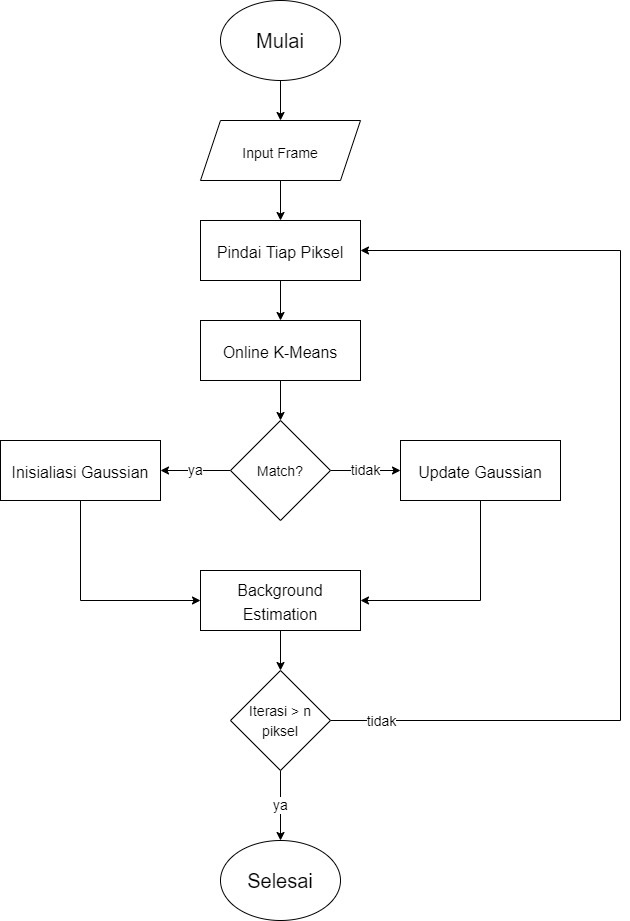
\includegraphics[width=8cm]{image/FlowChart-GMM.jpg}
          \caption{Diagram alir proses \textit{Background Subtraction} dengan GMM}
          \label{fig:gmmflowchart}
        \end{figure}
        
    \subsection{Proses Menghilangkan Noise Melalui Operasi Morfologi}
        Keluaran dari proses deteksi objek menggunakan metode \textit{Background Subtraction} dengan bantuan GMM adalah sebuah citra biner dengan nilai piksel $0$ sebagai latar belakang dan nilai piksel $1$ sebagai latar depan. Citra hasil keluaran proses tersebut masih berisikan banyak \textit{noise} (piksel latar depan yang bukan objek). Maka dari itu, operasi morfologi diperlukan untuk menghilangkan \textit{noise} tersebut.
        \begin{figure}[H]
        \centering
          \singlespacing
          \captionsetup{justification=centering,margin=0.5cm}
          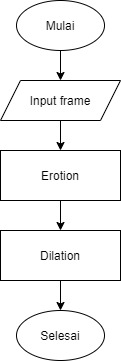
\includegraphics[width=4cm]{image/FlowChart-Morphology.jpg}
          \caption{Diagram alir Operasi Morfologi}
          \label{fig:morphologyflowchart}
        \end{figure}
        
        Citra biner akan melalui dua tahap operasi morfologi, yaitu erosi yang disusul oleh dilasi \textit{(opening)}. Erosi sesuai dengan namanya adalah proses pengikisan piksel. Dalam hal ini, erosi dapat menghilangkan \textit{noise} pada citra biner terutama \textit{salt and pepper noise} (derau kecil pada citra yang terlihat seperti garam bertaburan). \textit{Structuring element} yang akan digunakan oleh proses erosi berukuran $5 \times 5$ dengan bentuk kotak. Proses dilasi selanjutnya dilakukan untuk mengembalikan objek latar depan ke bentuk semula yang sebelumnya terkikis oleh proses erosi. Dilasi dapat memperbesar objek latar depan dan juga menyambungkan kembali bagian-bagian objek yang terpisah akibat proses erosi. \textit{Structuring element} yang akan digunakan oleh proses dilasi berukuran $11 \times 11$ dengan bentuk kotak. Keluaran yang diharapkan adalah citra biner yang bersih dari \textit{noise} serta objek latar depan yang utuh (tidak terpotong ataupun berlubang). Gambar \ref{fig:morphologyflowchart} memperlihatkan diagram alir dari alur operasi morfologi secara keseluruhan.
        
    \subsection{\textit{Downsampling} dan \textit{Contour Tracing}}
        \textit{Downsampling} terhadap sebuah \textit{frame} dijalankan sebelum algoritme CT dieksekusi. Hal ini dilakukan untuk meningkatkan perfoma CT. Algoritme dua dari metode \textit{contour tracing / border following} oleh Suzuki digunakan pada sistem ini. Algoritme dua hanya berfokus pada deteksi tepi bagian terluar \textit{(outer border)}, karena pada sistem kali ini tidak diperlukan deteksi tepi bagian dalam \textit{(hole border)}. Algoritme ini dijalankan dengan asumsi bahwa citra masukan merupakan citra biner dengan piksel bernilai 0 sebagai latar belakang dan piksel bernilai 1 sebagai latar depan (objek).
        
        Masukan berupa citra biner dari proses operasi morfologi yang kemudian dilakukan proses pemindaian \textit{(scan)} mulai dari piksel paling kiri atas. Ketika pemindai sampai pada sebuah piksel $(i, j)$ bernilai $f_{i, j} \neq 0$, ditentukan apakah piksel tersebut merupakan \textit{starting point} dari operasi \textit{border following} untuk tepi luar atau tepi dalam (Gambar \ref{fig:outerandholeborder}). Lalu \textit{parent border} untuk piksel $(i, j)$ ditentukan berdasarkan Gambar \ref{fig:parentborder}. Langkah selanjutnya adalah melakukan operasi \textit{border following} dimulai dari \textit{starting point} piksel $(i, j)$ sampai pointer kembali ke posisi \textit{starting point} (3.e). Dikarenakan algoritme yang digunakan adalah algoritme dua, nilai $NBD$ dan $-NBD$ akan diset masing-masing $2$ dan $-2$. Kemudian \textit{scanner} melanjutkan pemindaian untuk kembali mencari nilai piksel $f_{i, j} \neq 0$. Algoritme dinyatakan selesai apabila \textit{scanner} sudah sampai pada sudut kanan bawah (piksel terakhir).
        \begin{figure}[H]
        \centering
          \singlespacing
          \captionsetup{justification=centering,margin=0.5cm}
          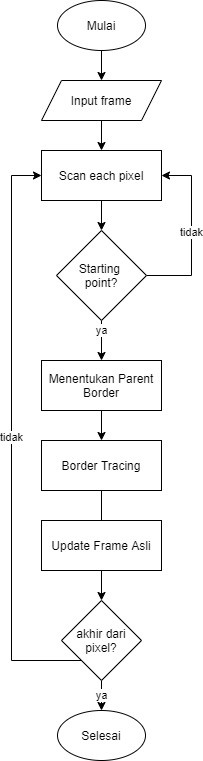
\includegraphics[width=4cm]{image/FlowChart-Countour.jpg}
          \caption{Diagram alir proses \textit{Contour Tracing}}
          \label{fig:countourtracingflowchart}
        \end{figure}
        
        Proses \textit{contour tracing} menghasilkan citra biner yang objek-objeknya sudah mempunyai tepi/konturnya masing-masing. Kemudian dari kontur tersebut dapat diekstraksi lebar dan tinggi sebuah objek. Dari nilai panjang dan lebar  itulah penulis dapat menggambarkan \textit{bounding box} untuk masing-masing objek tersebut.
        
    \subsection{\textit{Decision of Occlusion}, Asosiasi Data, dan Kalman Filter }
        Kalman Filter digunakan sebagai pelacak \textit{(tracker)} untuk masing-masing objek yang terdeteksi. Langkah pertama pada proses pelacakan objek adalah untuk menginisialisasi Kalman Filter sebanyak jumlah objek yang terdeteksi pada proses sebelumnya. Setiap Kalman Filter dikonfigurasikan sebagai berikut:
        \begin{equation}\label{eq:3.1}
        x_k = 
        \begin{bmatrix}
        p_k & q_k & l_k & h_k & v_{p, k} & v_{q, k}
        \end{bmatrix}^T
        \end{equation}
        
        Dimana $p_{k}$ dan $q_{k}$ merepresentasikan nilai horizontal dan vertikal koordinat titik tengah, $l_k$ dan $h_k$ merepresentasikan setengah dari lebar dan tinggi \textit{bounding box}, serta $v_{p, k}$ dan $v_{q, k}$ merepresentasikan kecepatan dari $p_{k}$ dan $q_{k}$.
        
        Kemudian untuk model pengukuran \textit{(measurement model)} yang digunakan oleh sistem ini didefinisikan sebagai berikut:
        \begin{equation}\label{eq:3.2}
        z_k = 
        \begin{bmatrix}
        p_k & q_k & l_k & h_k
        \end{bmatrix}^T
        \end{equation}
        
        Di bawah ini dimodelkan matriks transisi $F$ dan matriks transisi $H$ untuk masing-masing model proses dan model pengukuran:
        \begin{equation}\label{eq:3.3}
        F = 
        \renewcommand{\arraystretch}{1}
        \setlength\arraycolsep{8pt}
        \begin{bmatrix}
        1 & 0 & 0 & 0 & \Delta{t} & 0\\
        0 & 1 & 0 & 0 & 0 & \Delta{t}\\
        0 & 0 & 1 & 0 & 0 & 0\\
        0 & 0 & 0 & 1 & 0 & 0\\
        0 & 0 & 0 & 0 & 1 & 0\\
        0 & 0 & 0 & 0 & 0 & 1
        \end{bmatrix}
        \end{equation}
        
        \begin{equation}\label{eq:3.4}
        H = 
        \renewcommand{\arraystretch}{1}
        \setlength\arraycolsep{9.5pt}
        \begin{bmatrix}
        1 & 0 & 0 & 0 & 0 & 0\\
        0 & 1 & 0 & 0 & 0 & 0\\
        0 & 0 & 1 & 0 & 0 & 0\\
        0 & 0 & 0 & 1 & 0 & 0
        \end{bmatrix}
        \end{equation}
        
        Setelah melalui proses pendefinisian model proses dan model pengukuran di atas, Kalman Filter kemudian dapat digunakan untuk memperkirakan lokasi serta ukuran sebuah objek pada \textit{frame} selanjutnya. Diagram alir untuk proses Kalman Filter dapat dilihat pada Gambar \ref{fig:kalmanfilterflowchart}.
        \begin{figure}[H]
        \centering
          \singlespacing
          \captionsetup{justification=centering,margin=0.5cm}
          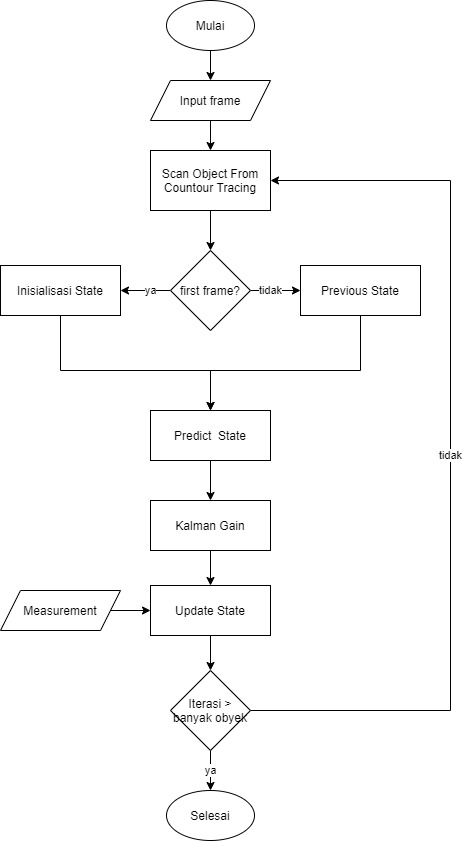
\includegraphics[width=9cm]{image/FlowChart-Kalman Filter.jpg}
          \caption{Diagram alir proses pelacakan dengan Kalman Filter}
          \label{fig:kalmanfilterflowchart}
        \end{figure}
        
        Pada proses ini, Kalman Filter membutuhkan variabel $z_k$ yang didapatkan dari hasil deteksi objek. Untuk menentukan objek hasil deteksi mana yang sesuai dengan prediksi Kalman Filter, dilakukan proses asosiasi data terhadap jarak serta variasi luas antara objek yang diestimasi dengan objek yang dideteksi. Selain itu, proses \textit{decision of occlusion} juga dilakukan untuk menentukan apakah terdapat objek yang mengalami proses \textit{merging} ataupun \textit{splitting}. Setiap objek yang mengalami proses \textit{merging} dengan objek lainnya akan menghasilkan objek baru yang kemudian dipasangkan dengan Kalman Filternya sendiri. Objek baru tersebut akan terus dilacak sampai proses \textit{splitting} terjadi.
        
        \begin{figure}[H]
        \centering
          \singlespacing
          \captionsetup{justification=centering,margin=0.5cm}
          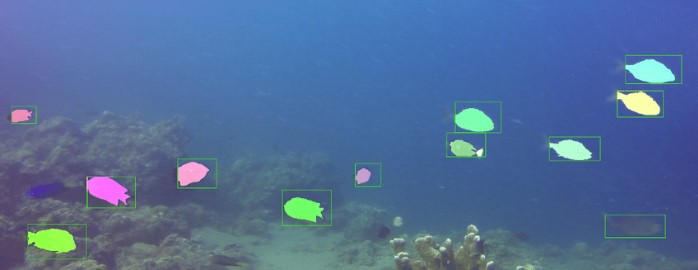
\includegraphics[width=13cm]{image/example_result.jpg}
          \caption{Contoh keluaran sistem}
          \small{Sumber: \href{https://www.researchgate.net/figure/Large-Frame-Fish-Detection-and-Instance-Segmentation_fig1_332153021}{ResearchGate}}
          \label{fig:example_result}
        \end{figure}
        
\section{Perancangan Eksperimen}

    Pada subbab ini akan dibahas mengenai rancangan eksperimen yang akan dilakukan pada penelitian ini. Eksperimen diawali dengan pengambilan data, kemudian dilanjutkan dengan pelacakan oleh sistem, dan terakhir evaluasi hasil.

    \subsection{Sumber Data}
        Berdasarkan sumber datanya, dataset pada penelitian ini akan dibagi menjadi dua. Secara keseluruhan, pengujian dalam penelitian ini dilakukan terhadap video ikan yang sudah direkam sebelumnya \textit{(offline tracking)}. Video tersebut kemudian dimasukkan sebagai input sistem dengan pengaturan bawaan \textit{(default)}. Pengaturan parameter dapat disesuaikan dengan kebutuhan pengguna untuk mendapatkan hasil pelacakan yang optimal.
        
        Dataset didapatkan dari sumber internet. Diunduh dari situs \href{https://alzayats.github.io/DeepFish/}{\textit{DeepFish}} \citep{Saleh2020} dan \href{http://www.perceivelab.com/datasets}{\textit{PeRCeiVeLab}} \citep{Kavasidis2012}. Dataset yang diunduh dari situs \href{https://alzayats.github.io/DeepFish/}{\textit{DeepFish}} berupa kumpulan gambar \textit{frame} video yang kemudian diubah ke dalam bentuk video dengan format mp4 dengan resolusi 720 x 480 dan \textit{frame rate} 24 fps. Sementara itu, dataset yang diunduh dari situs \href{http://www.perceivelab.com/datasets}{\textit{PeRCeiVeLab}} merupakan video dengan format \textit{flv} berdurasi 9 menit dan dengan resolusi 320x240 serta \textit{frame rate} 8 fps. Berdasarkan jumlah ikan dan keadaan latar belakang, terdapat empat skenario pengujian yang akan dilakukan pada penelitian ini. Keempat skenario tersebut adalah:
            \begin{enumerate}
                \item Pengujian terhadap video berisikan satu ikan dengan latar belakang sederhana
                \item Pengujian terhadap video berisikan satu ikan dengan latar belakang kompleks
                \item Pengujian terhadap video berisikan dua atau lebih ikan \textit{(multiple object)} dengan latar belakang sederhana
                \item Pengujian terhadap video berisikan dua atau lebih ikan \textit{(multiple object)} dengan latar belakang kompleks
            \end{enumerate}
        Secara keseluruhan, terdapat empat video yang akan digunakan dalam penelitian ini. Dataset video yang diambil sebagai masukan sistem adalah sebagai berikut:
            \begin{enumerate}
                \item Video skenario pengujian satu diambil dari situs \href{https://alzayats.github.io/DeepFish/}{\textit{DeepFish}} 
                indeks 9908 berdurasi 12 detik (24fps). Video ini digunakan karena latar belakang video termasuk ke dalam kategori sederhana.
                \vspace{-0.5cm}
                \begin{figure}[H]
                \centering
                  \singlespacing
                  \captionsetup{justification=centering,margin=0.5cm}
                  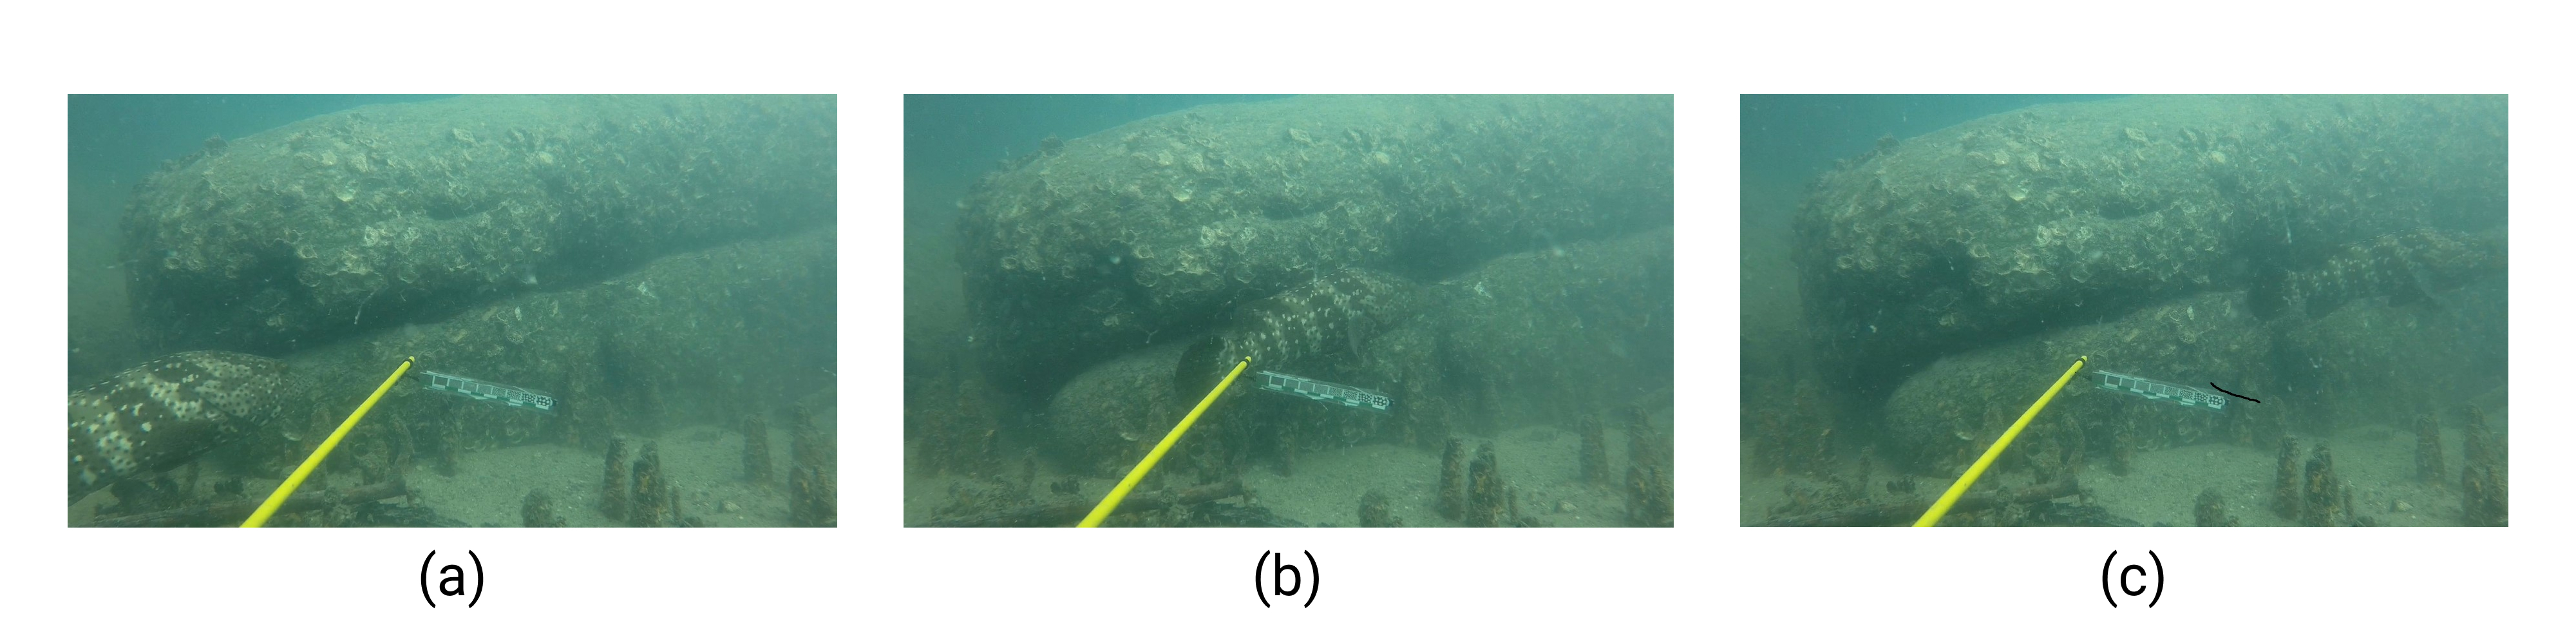
\includegraphics[width=12cm]{image/sample_frame_9908.jpg}
                  \caption{Sampel \textit{frame} video dataset \textit{DeepFish} indeks 9908}
                  \small{Sumber: \href{https://alzayats.github.io/DeepFish/}{\textit{DeepFish Video Dataset}}}
                  \label{fig:sample_9908}
                \end{figure}
                \item Video skenario pengujian dua diambil dari situs \href{https://alzayats.github.io/DeepFish/}{\textit{DeepFish}} 
                indeks 9866 berdurasi 35 detik (24fps). Video ini digunakan karena latar belakang video termasuk ke dalam kategori kompleks (dinamis).
                \vspace{-0.5cm}
                \begin{figure}[H]
                \centering
                  \singlespacing
                  \captionsetup{justification=centering,margin=0.5cm}
                  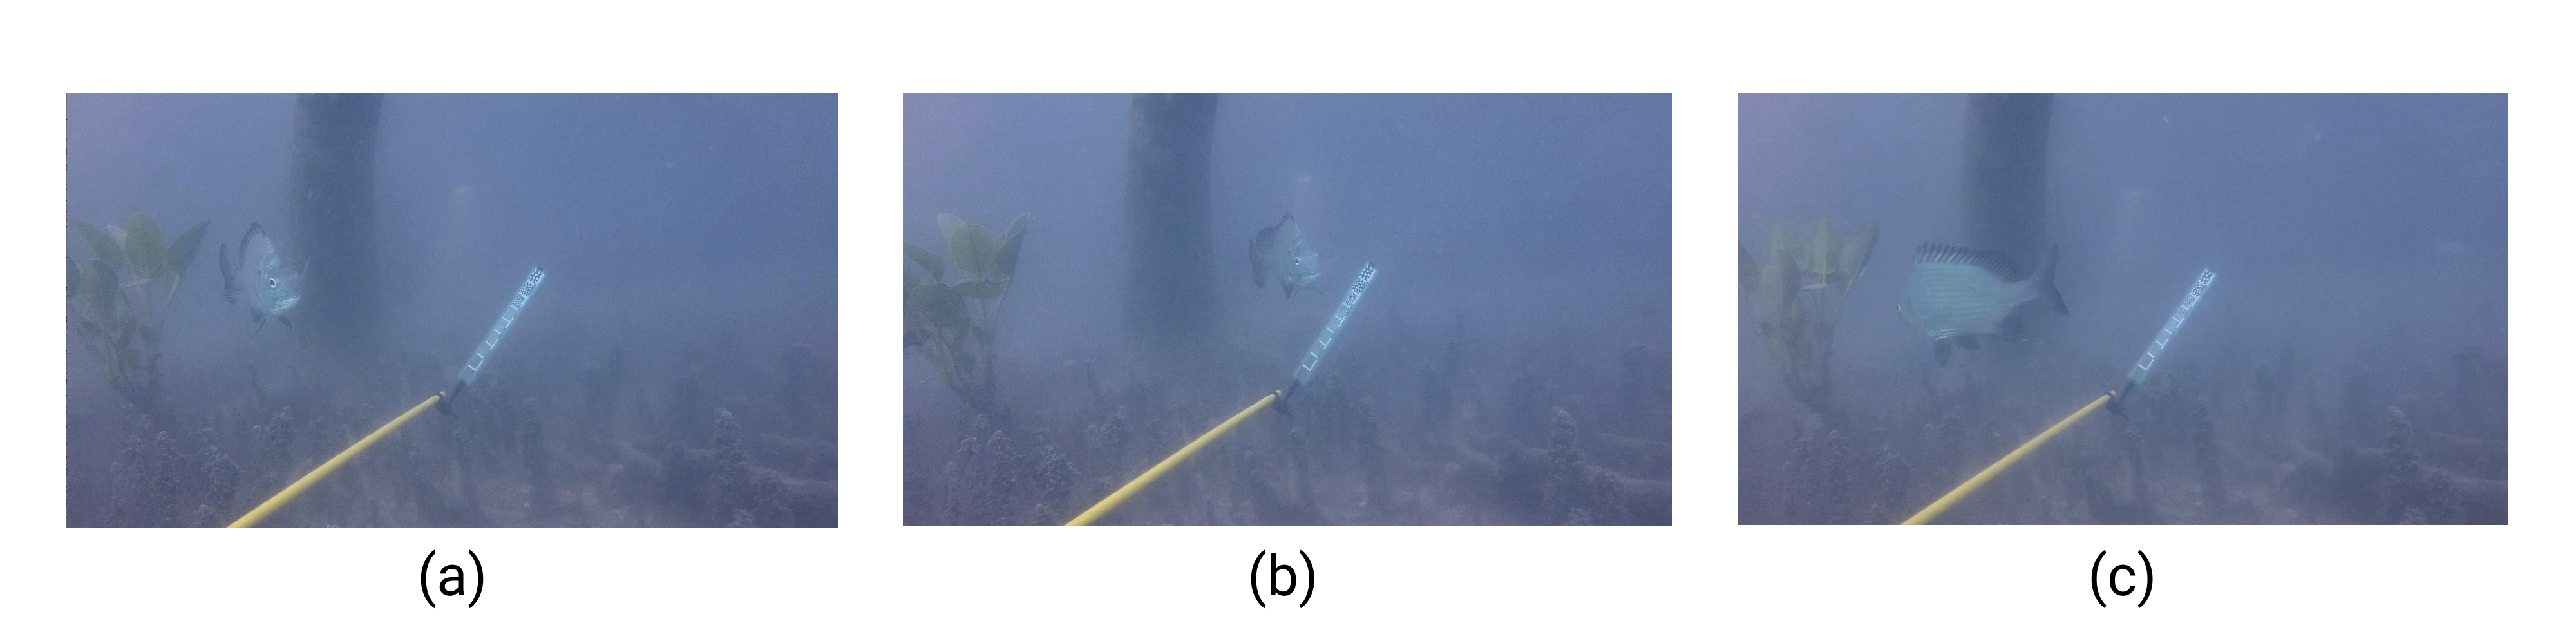
\includegraphics[width=12cm]{image/sample_frame_9866.jpg}
                  \caption{Sampel \textit{frame} video dataset \textit{DeepFish} indeks 9866}
                  \small{Sumber: \href{https://alzayats.github.io/DeepFish/}{\textit{DeepFish Video Dataset}}}
                  \label{fig:sample_9866}
                \end{figure}
                \item Video skenario pengujian tiga diambil dari situs \href{http://www.perceivelab.com/datasets}{\textit{PeRCeiVeLab}}
                indeks gt\textunderscore 124 berdurasi 9 menit 22 detik (8fps) yang telah dipotong menjadi 2 menit 30 detik. Video ini digunakan karena sudah cukup memenuhi kriteria skenario pengujian ke-tiga, yaitu jumlah objek lebih dari satu dengan latar belakang sederhana.
                \vspace{-0.5cm}
                \begin{figure}[H]
                \centering
                  \singlespacing
                  \captionsetup{justification=centering,margin=0.5cm}
                  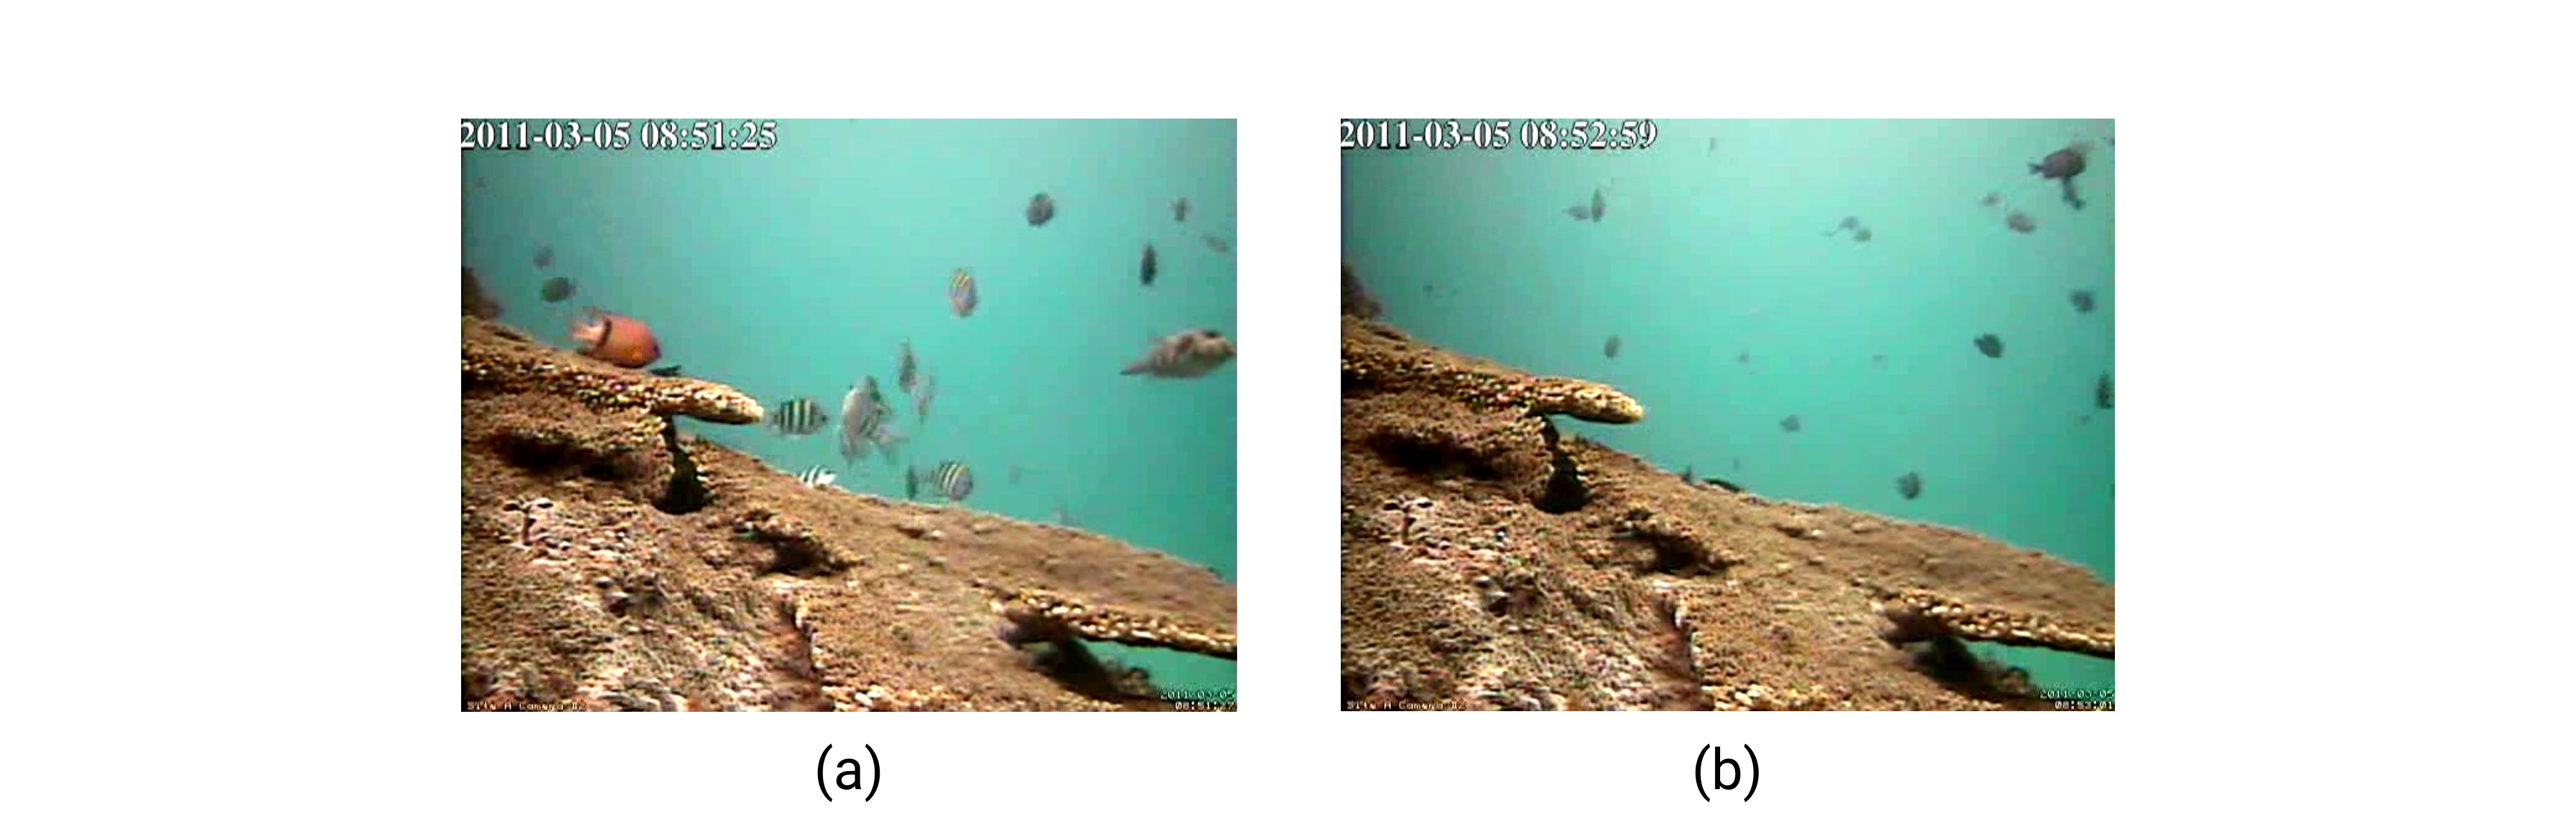
\includegraphics[width=12cm]{image/sample_frame_gt_124.jpg}
                  \caption{Sampel \textit{frame} video dataset \textit{PeRCeiVeLab} indeks gt\textunderscore 124}
                  \small{Sumber: \href{https://alzayats.github.io/DeepFish/}{\textit{DeepFish Video Dataset}}}
                  \label{fig:sample_9866}
                \end{figure}
                \item Video skenario pengujian empat diambil dari situs \href{http://www.perceivelab.com/datasets}{\textit{PeRCeiVeLab}}
                indeks gt\textunderscore 116 berdurasi 9 menit 35 detik (8fps) yang telah dipotong menjadi 2 menit 30 detik. Video ini digunakan karena sudah cukup memenuhi kriteria skenario pengujian ke-empat, yaitu jumlah objek lebih dari satu dengan latar belakang kompleks.
                \vspace{-0.5cm}
                \begin{figure}[H]
                \centering
                  \singlespacing
                  \captionsetup{justification=centering,margin=0.5cm}
                  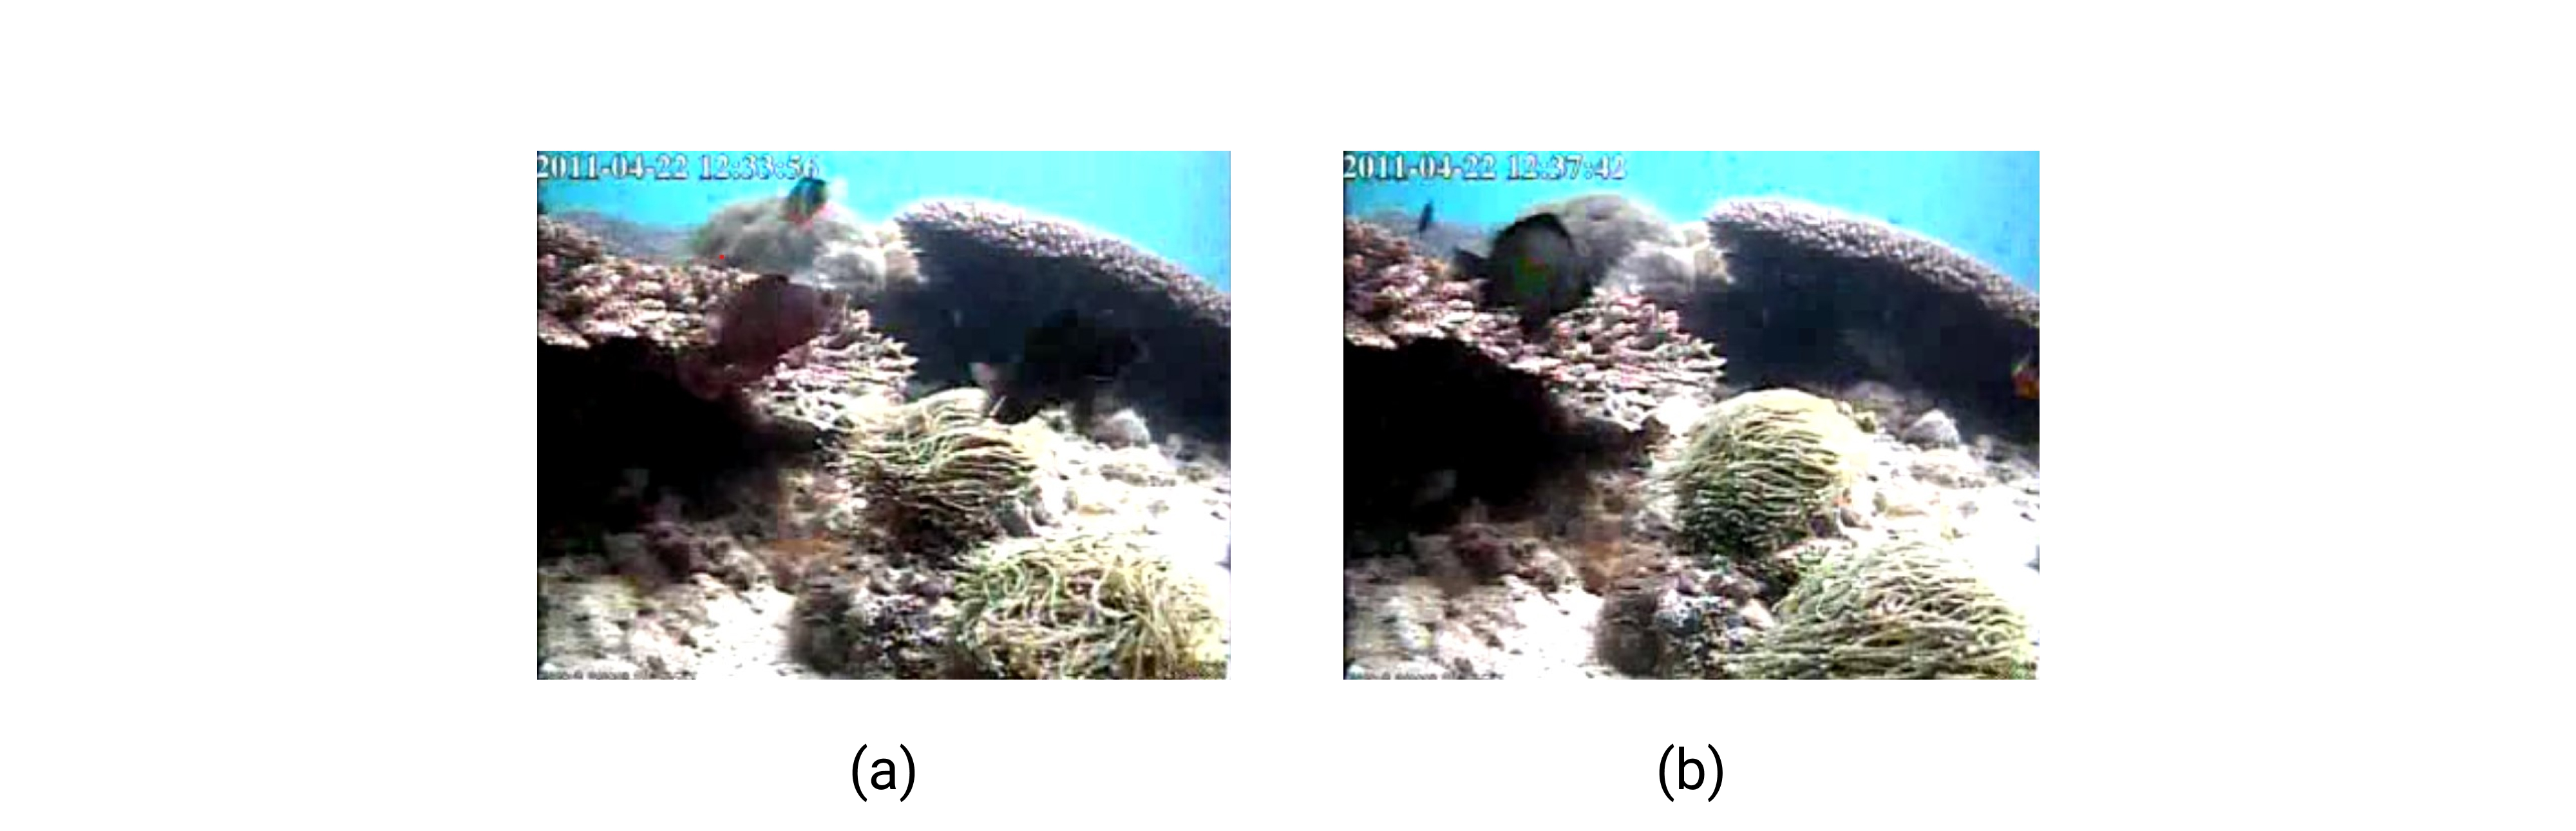
\includegraphics[width=14cm]{image/sample_frame_gt_116.jpg}
                  \caption{Sampel \textit{frame} video dataset \textit{PeRCeiVeLab} indeks gt\textunderscore 116}
                  \small{Sumber: \href{https://alzayats.github.io/DeepFish/}{\textit{DeepFish Video Dataset}}}
                  \label{fig:sample_9866}
                \end{figure}
            \end{enumerate}
        
    \subsection{Evaluasi Hasil}
    Pada subbab ini akan dijelaskan terkait validasi / pembuktian kebenaran dari metode-metode utama pada penelitian ini. Metode-metode tersebut adalah GMM, \textit{Contour Tracing}, dan Kalman Filter. Adapun pembuktian metode-metode tersebut dapat dijabarkan sebagai berikut.
    
        \setlist{ listparindent=\parindent, parsep=0pt}
        \begin{enumerate}
            \item GMM dan Morfologi
            
            Masukan dari metode ini dapat berupa citra RGB ataupun citra biner. Keluaran yang dihasilkan dari metode GMM adalah citra biner dengan piksel bernilai 0 sebagai latar belakang dan piksel bernilai 1 sebagai latar depan (objek). Hasil dari metode ini dapat dikatakan baik apabila ekstraksi latar depan sudah sesuai dengan objek bergerak yang ingin dilacak, dalam kasus ini yaitu objek ikan. Sebaliknya, jika objek selain ikan ikut terekstrak sebagai bagian dari latar depan (latar belakang dinamis, gelembung air), maka sistem dianggap kurang baik.
            
            \begin{figure}[H]
            \centering
              \singlespacing
              \captionsetup{justification=centering,margin=0.5cm}
              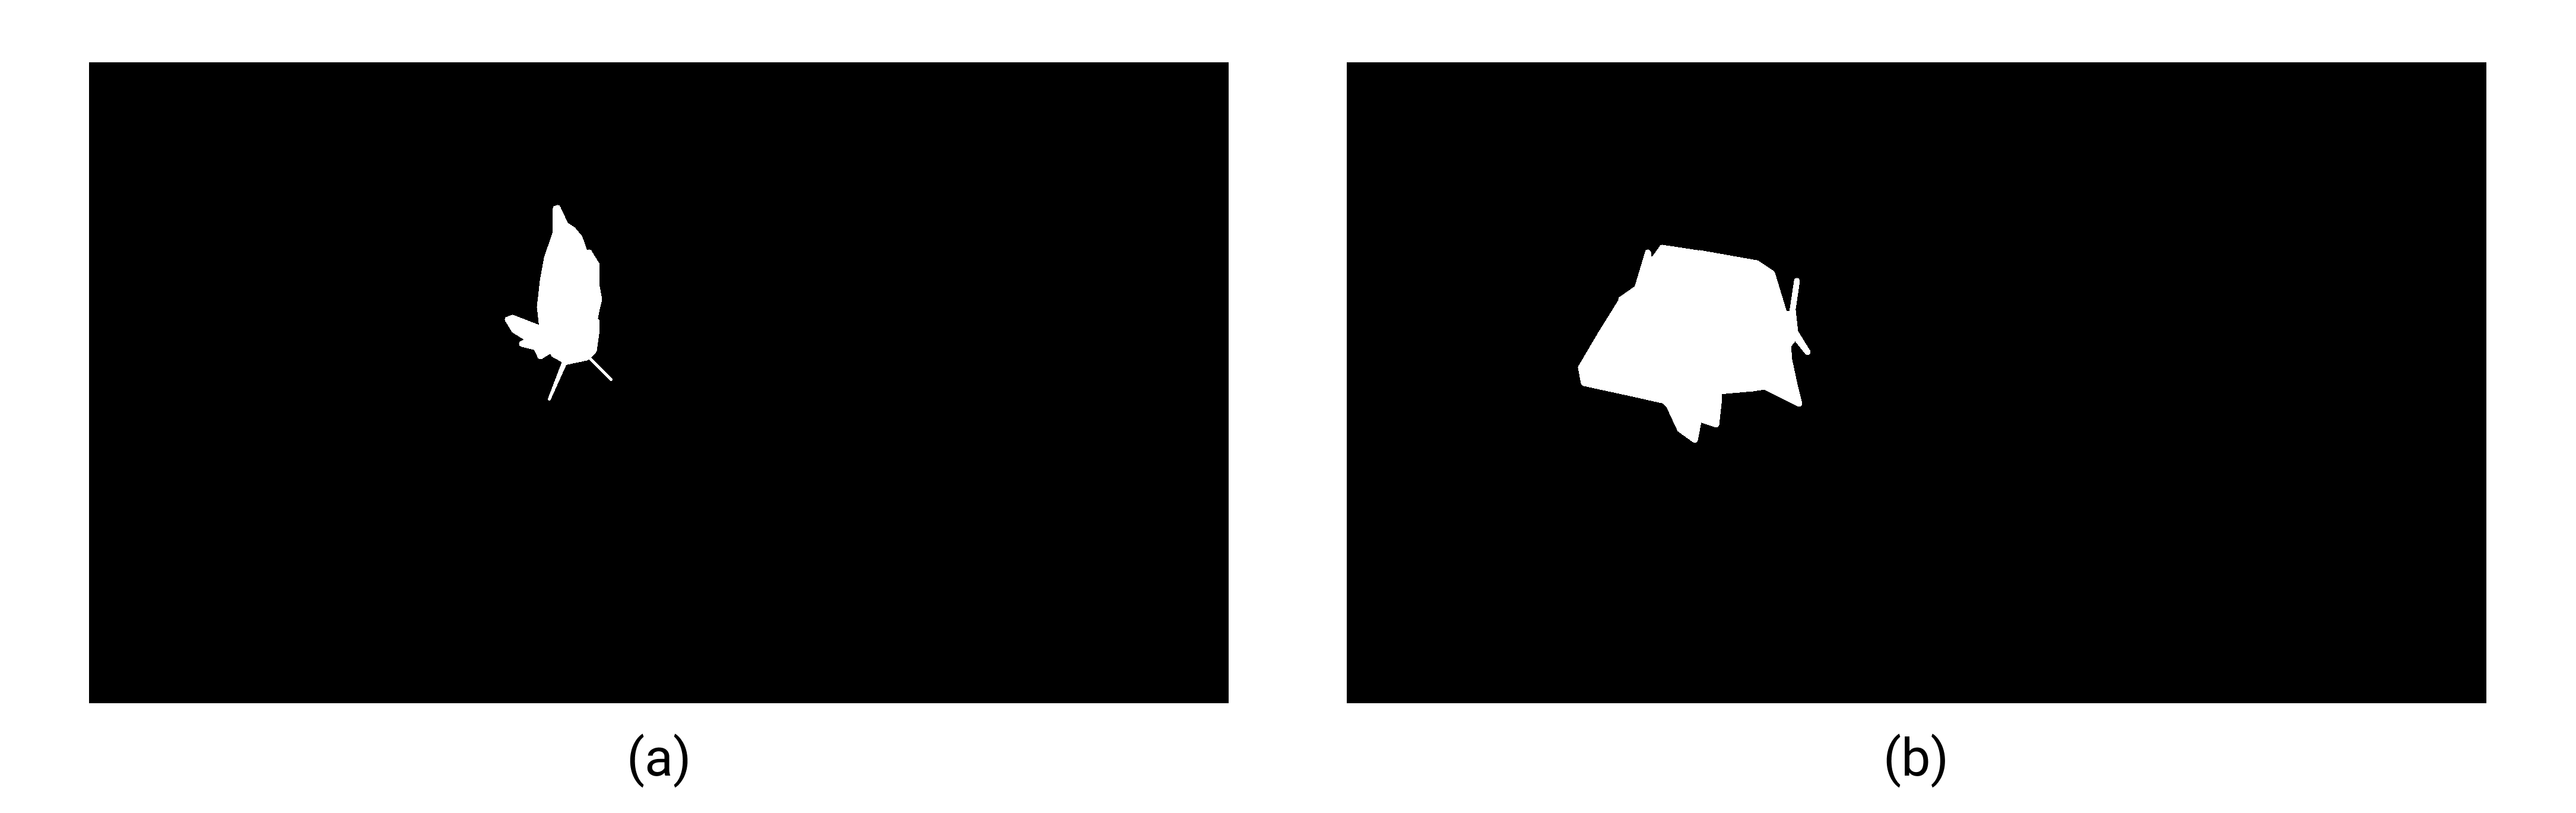
\includegraphics[width=10cm]{image/gt1.jpg}
              \caption{Contoh \textit{groundtruth} GMM}
              \label{fig:gt1}
            \end{figure}
            
            Performa metode GMM dihitung dengan cara membandingkan hasil deteksi objek dengan \textit{groundtruth} (Gambar \ref{fig:gt1}). Sebanyak 3 (tiga) sampel \textit{groundtruth} diambil dari masing-masing video. Empat buah variabel, $A$ \textit{(Accuracy)}, $P$ \textit{(Precision)}, $R$ \textit{(Recall)}, $F1$ \textit{(F1 Score)} dan digunakan untuk mengukur performa metode sebagai berikut:
            
            \begin{equation}\label{eq:3.5}
           	A = \frac{TN + TP}{TN + FP + TP + FN} \times 100 \%
            \end{equation}
            
            \begin{equation}\label{eq:3.5}
            P = \frac{TP}{TP + FP} \times 100 \%
            \end{equation}
            
            \begin{equation}\label{eq:3.6}
            R = \frac{TP}{TP + FN} \times 100 \%
            \end{equation}
        
	        \begin{equation}\label{eq:3.6}
        	F1 = 2 \cdot \frac{P \cdot R}{P + R} \times 100 \%
	        \end{equation}
            
            dimana $A$ merepresentasikan jumlah piksel yang dideteksi dari seluruh deteksi adalah benar latar depan,  $P$ \textit{(Precision)} merepresentasikan seberapa besar persentase piksel yang diprediksi adalah benar latar depan, $R$ \textit{(Recall)} merepresentasikan seberapa besar persentase piksel latar depan yang berhasil dideteksi, $F1$ merupakan gabungan dari \textit{Recall} dan \textit{Precision}, $TP$ \textit{(True Positive)} adalah hasil deteksi piksel latar depan yang benar, $TN$ \textit{(True Negative)} adalah hasil deteksi piksel latar belakang yang benar, $FP$ \textit{(False Positive)} adalah piksel latar belakang yang terdeteksi sebagai piksel latar depan, dan $FN$ \textit{(False Negative)} adalah piksel latar depan yang tidak terdeteksi oleh sistem \citep{Chavan2017}. Performa metode GMM dapat dikatakan baik apabila variabel $P$ dan $R$ menghasilkan nilai persentase yang besar.
            
            \item \textit{Downsampling}

            Metode \textit{Downsapling} diperlukan untuk meningkatkan performa 
            \textit{tracing} pada metode CT dengan memperhitungkan juga akurasi sistem serta kualitas gambar. Tiga $(3)$ buah sampel diambil dari masing-masing video. Evaluasi dihitung dengan cara membandingkan waktu eksekusi metode CT sebelum dan sesudah dilakukan \textit{downsampling} pada \textit{frame} terkait.
            
            \item \textit{Contour Tracing}
            
            Metode CT mengambil masukan citra biner dari proses deteksi objek bergerak sebelumnya. Metode ini menghasilkan citra biner yang setiap objek bergerak sudah mempunyai tepi / konturnya masing-masing. Dari kontur tersebut dapat dihasilkan \textit{bounding box}. Pembuktian dapat dilakukan dengan cara membandingkan jumlah objek / jumlah kontur hasil metode CT dengan \textit{groundtruth}. Sebanyak $3$ (tiga) buah sampel \textit{groundtruth} diambil dari masing-masing video. Dua atau lebih objek yang mengalami proses \textit{occlusion} dapat diklasifikasikan sebagai satu objek. \textit{Absolute Error} digunakan dalam proses evaluasi metode CT.
            \begin{equation}\label{eq:3.7}
            \text{AE} = \bigg|\frac{\textit{Jumlah objek sebenarnya - Jumah objek hasil CT}}{\textit{Jumah objek hasil CT}}\bigg| \times 100\%
            \end{equation}
            
            Nilai $\textit{Absolute Error} =  0\%$ menyatakan bahwa jumlah objek sudah sesuai dengan \textit{groundtruth}. Performa metode CT sangat bergantung pada hasil deteksi objek dari metode sebelumnya. Maka dari itu, jika nilai $\textit{error}$ cukup besar, perlu dilakukan penyesuaian parameter sistem untuk kemudian dilakukan pengujian ulang agar mendapatkan hasil yang baik.
            \begin{figure}[H]
            \centering
              \singlespacing
              \captionsetup{justification=centering,margin=0.5cm}
              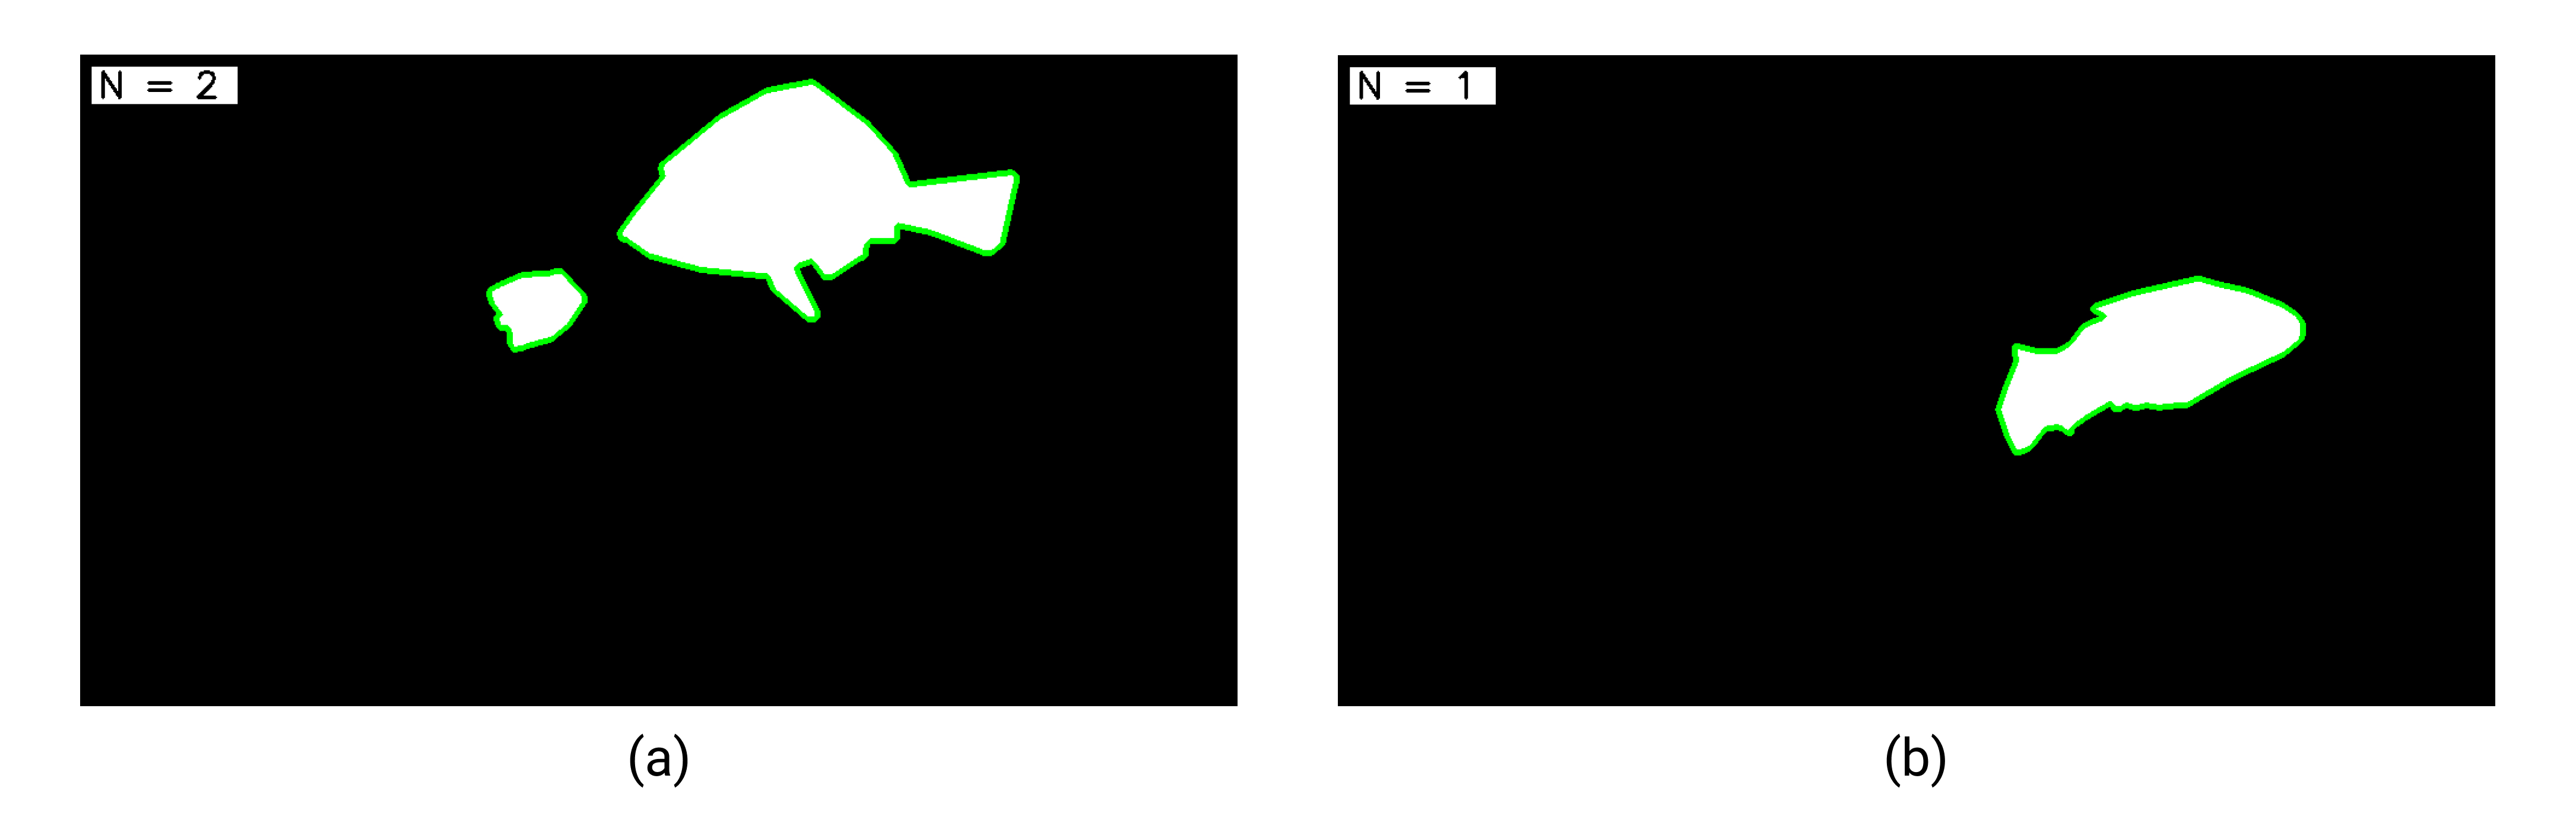
\includegraphics[width=10cm]{image/gt_ct.jpg}
              \caption{Contoh \textit{groundtruth} \textit{Contour Tracing}}
              \label{fig:gt1}
            \end{figure}
            
            \item Pelacakan Objek dengan Kalman Filter
            
            Kalman Filter bertugas sebagai pemberi label/identitas untuk setiap objek yang mempunyai \textit{bounding box}. Proses asosiasi data membuat Kalman Filter dapat mempertahankan label masing-masing objek tersebut selama video berlangsung. Inilah yang disebut sebagai proses "pelacakan objek". Keluaran dari proses ini adalah \textit{running} video berisikan objek yang dilacak lengkap dengan \textit{bounding box} serta label uniknya masing-masing. 
            
            Performa metode Kalman Filter dihitung dengan cara membandingkan hasil pelacakan oleh sistem dengan \textit{groundtruth} berupa koordinat nilai tengah masing-masing objek. Sampel \textit{groundtruht} diambil dari masing-masing video sebanyak 3 sampel. \textit{Root Mean Squared Error} \textit{(RMSE)} digunakan untuk mengukur performa nilai yang diprediksi oleh  model \textit{(predicted)} dengan nilai sebenarnya \textit{(observed)}. Formula \textit{RMSE} dapat didefinisikan sebagai berikut: 
            \begin{equation}\label{eq:3.8}
            \textit{TOTAL RMSE} = \sqrt{(RMSE_X)^2 + (RMSE_Y)^2}
            \end{equation}
            dimana
            \begin{equation}\label{eq:3.9}
            RMSE_X = \sqrt{\sum_{i = 1}^n  \frac{(\hat{x}_i - x_i)^2}{n}}
            \end{equation}
            \begin{equation}\label{eq:3.10}
            RMSE_Y = \sqrt{\sum_{i = 1}^n  \frac{(\hat{y}_i - y_i)^2}{n}}
            \end{equation}
            
            Variabel $\hat{x}_i$, $\hat{y}_i$ adalah nilai koordinat titik tengah $(x, y)$ yang diprediksi, sementara $x_i$, $y_i$ adalah nilai koordinat titik tengah $(x, y)$ yang diobservasi, dan $n$ adalah jumlah observasi. Hasil pelacakan dapat dikatakan baik apabila nilai \textit{TOTAL RMSE} mendekati 0.
        \end{enumerate}
    
    \subsection{Parameter Sistem}
    
    Dalam sistem pelacakan ini, terdapat beberapa parameter yang perlu diatur demi mendapatkan hasil pelacakan yang optimal. Pengujian \textit{tuning} parameter dilakukan terhadap seluruh skenario pengujian masing-masing metode pada subbab sebelumnya.
        \begin{enumerate}
            \item \textit{Downsampling Scale}
            
            Besaran skala dalam proses \textit{Downsampling} berfungsi sebagai penentu seberapa besar sistem akan melakukan \textit{Downsampling} terhadap sebuah \textit{frame} sebelum dilakukannya proses \textit{Contour Tracing}. Besaran skala yang digunakan adalah $S = 2,\, 4,\, 8$. Dengan mempertimbangkan kualitas gambar yang dihasilkan dan juga akurasi metode, penentuan besaran skala ini diharapkan dapat meningkatkan performa sistem secara signifikan.
            
            \item Ukuran \textit{Structuring Element}
            
            Terdapat dua \textit{structuring element} yang digunakan pada operasi morfologi. Ukuran bawaan \textit{structuring element} proses erosi adalah $5 \times 5$. Semakin besar ukurannya maka semakin banyak \textit{salt-pepper noise} yang hilang, akan tetapi semakin banyak pula piksel \textit{foreground} yang terkikis. Sementara itu,  ukuran bawaan \textit{structuring element} proses dilasi adalah $7 \times 7$. Semakin besar ukurannya, maka akan semakin baik sistem dalam menyambungkan bagian objek yang terputus ataupun berlubang, akan tetapi semakin besar juga kemungkinan dua buah objek yang seharusnya terpisah menjadi satu.
        \end{enumerate}
    
        
    
% \section{Jadwal Kegiatan}
% 	Quo no atqui omnesque intellegat, ne nominavi argumentum quo. Eum ei purto oporteat dissentiet, soleat utamur an sit. Et assum dicam interpretaris quo. Cetero alterum ea vel, no possit alterum utroque nec. His fuisset quaestio ad. Has eu tritani incorrupte consequuntur, esse aliquip nec ne \ref{jadwal}.

% 	% Please remember to add \use{multirow} to your document preamble in order to suppor multirow cells
% 		\begin{table}[H]
% 		\centering
% 		\caption{Jadwal Penelitian.}
% 		\label{jadwal}
% 		\begin{tabular}{|c|l|l|l|l|l|l|l|}
% 		\hline
% 		\multirow{2}{*}{No} & \multirow{2}{*}{Keterangan} & \multicolumn{6}{c|}{Bulan}                                                                                                                          \\ \cline{3-8} 
% 		                    &                             & 1 & 2 & 3 & 4 & 5 & 6 \\ \hline
% 		1                   & Studi literatur                                  &\cellcolor{gray} &\cellcolor{gray}&                        &                        &                        &                         \\ \hline
% 		2                   & Desain                                           &                        &\cellcolor{gray}&\cellcolor{gray}&                        &                        &                         \\ \hline
% 		3                   & Pembelian bahan                                  &                        &                        &\cellcolor{gray}&                        &                        &                         \\ \hline
% 		4                   & Pembuatan prototipe                              &                        &                        &\cellcolor{gray}&\cellcolor{gray}&\cellcolor{gray}&                         \\ \hline
% 		5                   & Uji coba dan perbaikan                           &                        &                        &                        &\cellcolor{gray}&\cellcolor{gray}&                         \\ \hline
% 		6                   & Penulisan skripsi                                &                        &                        &                        &                        &                        &\cellcolor{gray}\\ \hline
% 		\end{tabular}
% 		\end{table}
	
% Baris ini digunakan untuk membantu dalam melakukan sitasi
% Karena diapit dengan comment, maka baris ini akan diabaikan
% oleh compiler LaTeX.
\begin{comment}
\bibliography{daftar-pustaka}
\end{comment}


%!TEX root = ./template-skripsi.tex
%-------------------------------------------------------------------------------
%                            BAB IV
%               		HASIL DAN PEMBAHASAN
%-------------------------------------------------------------------------------

\chapter{HASIL DAN PEMBAHASAN}
    \section{Input Video}
        Pada tahap pertama, sumber data berupa video dimasukkan kedalam sistem yang kemudian diubah menjadi sekumpulan citra \textit{(frame)}. Kemudian citra melalui proses \textit{pre-processing}, yaitu konversi ruang warna RGB ke ruang warna \textit{grayscale}.
        \vspace{-0.5cm}
        \begin{figure}[H]
        \centering
          \singlespacing
          \captionsetup{justification=centering,margin=0.5cm}
          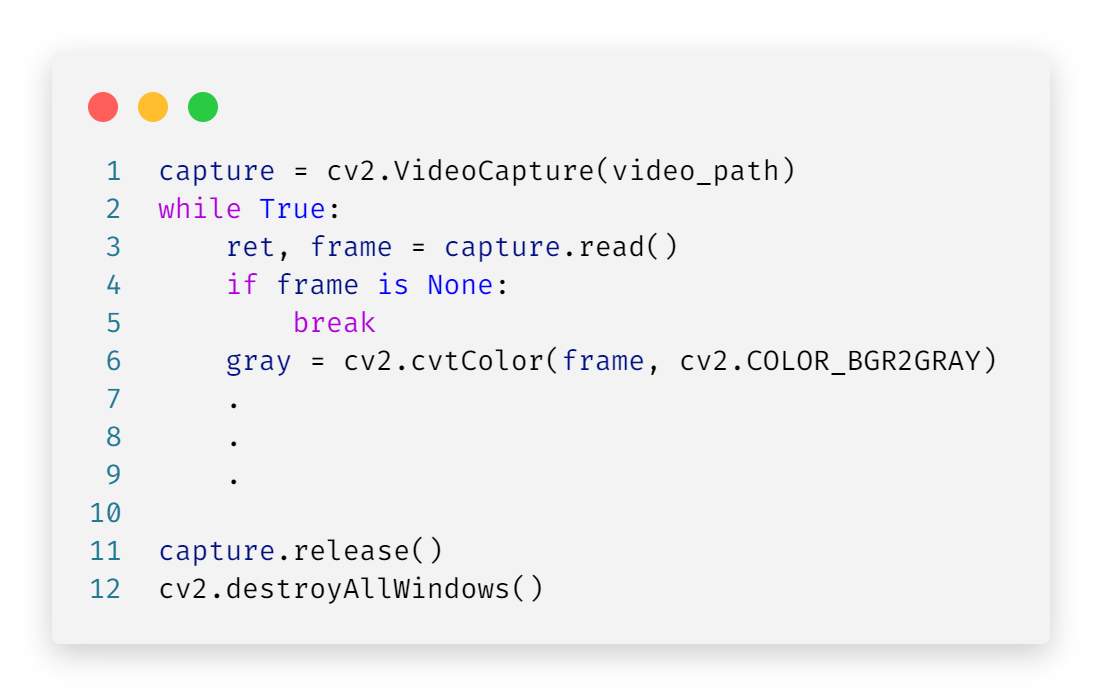
\includegraphics[width=12cm]{image/input.png}
          \caption{Potongan sampel kode input sistem}
          \label{fig:Potongan sampel kode input sistem}
        \end{figure}

    \section{GMM}
        Citra yang telah melalui proses \textit{pre-processing} selanjutnya digunakan sebagai data masukan proses \textit{background subtraction} menggunakan GMM. Keluaran dari metode ini kemudian dievaluasi terhadap \textit{groundtruth} yang sudah dipersiapkan sebelumnya. Diperoleh skor \textit{accuracy, recall, precision,} dan \textit{F1} untuk masing-masing data uji.

        \vspace{-0.5cm}
        \begin{figure}[H]
        \centering
          \singlespacing
          \captionsetup{justification=centering,margin=0.5cm}
          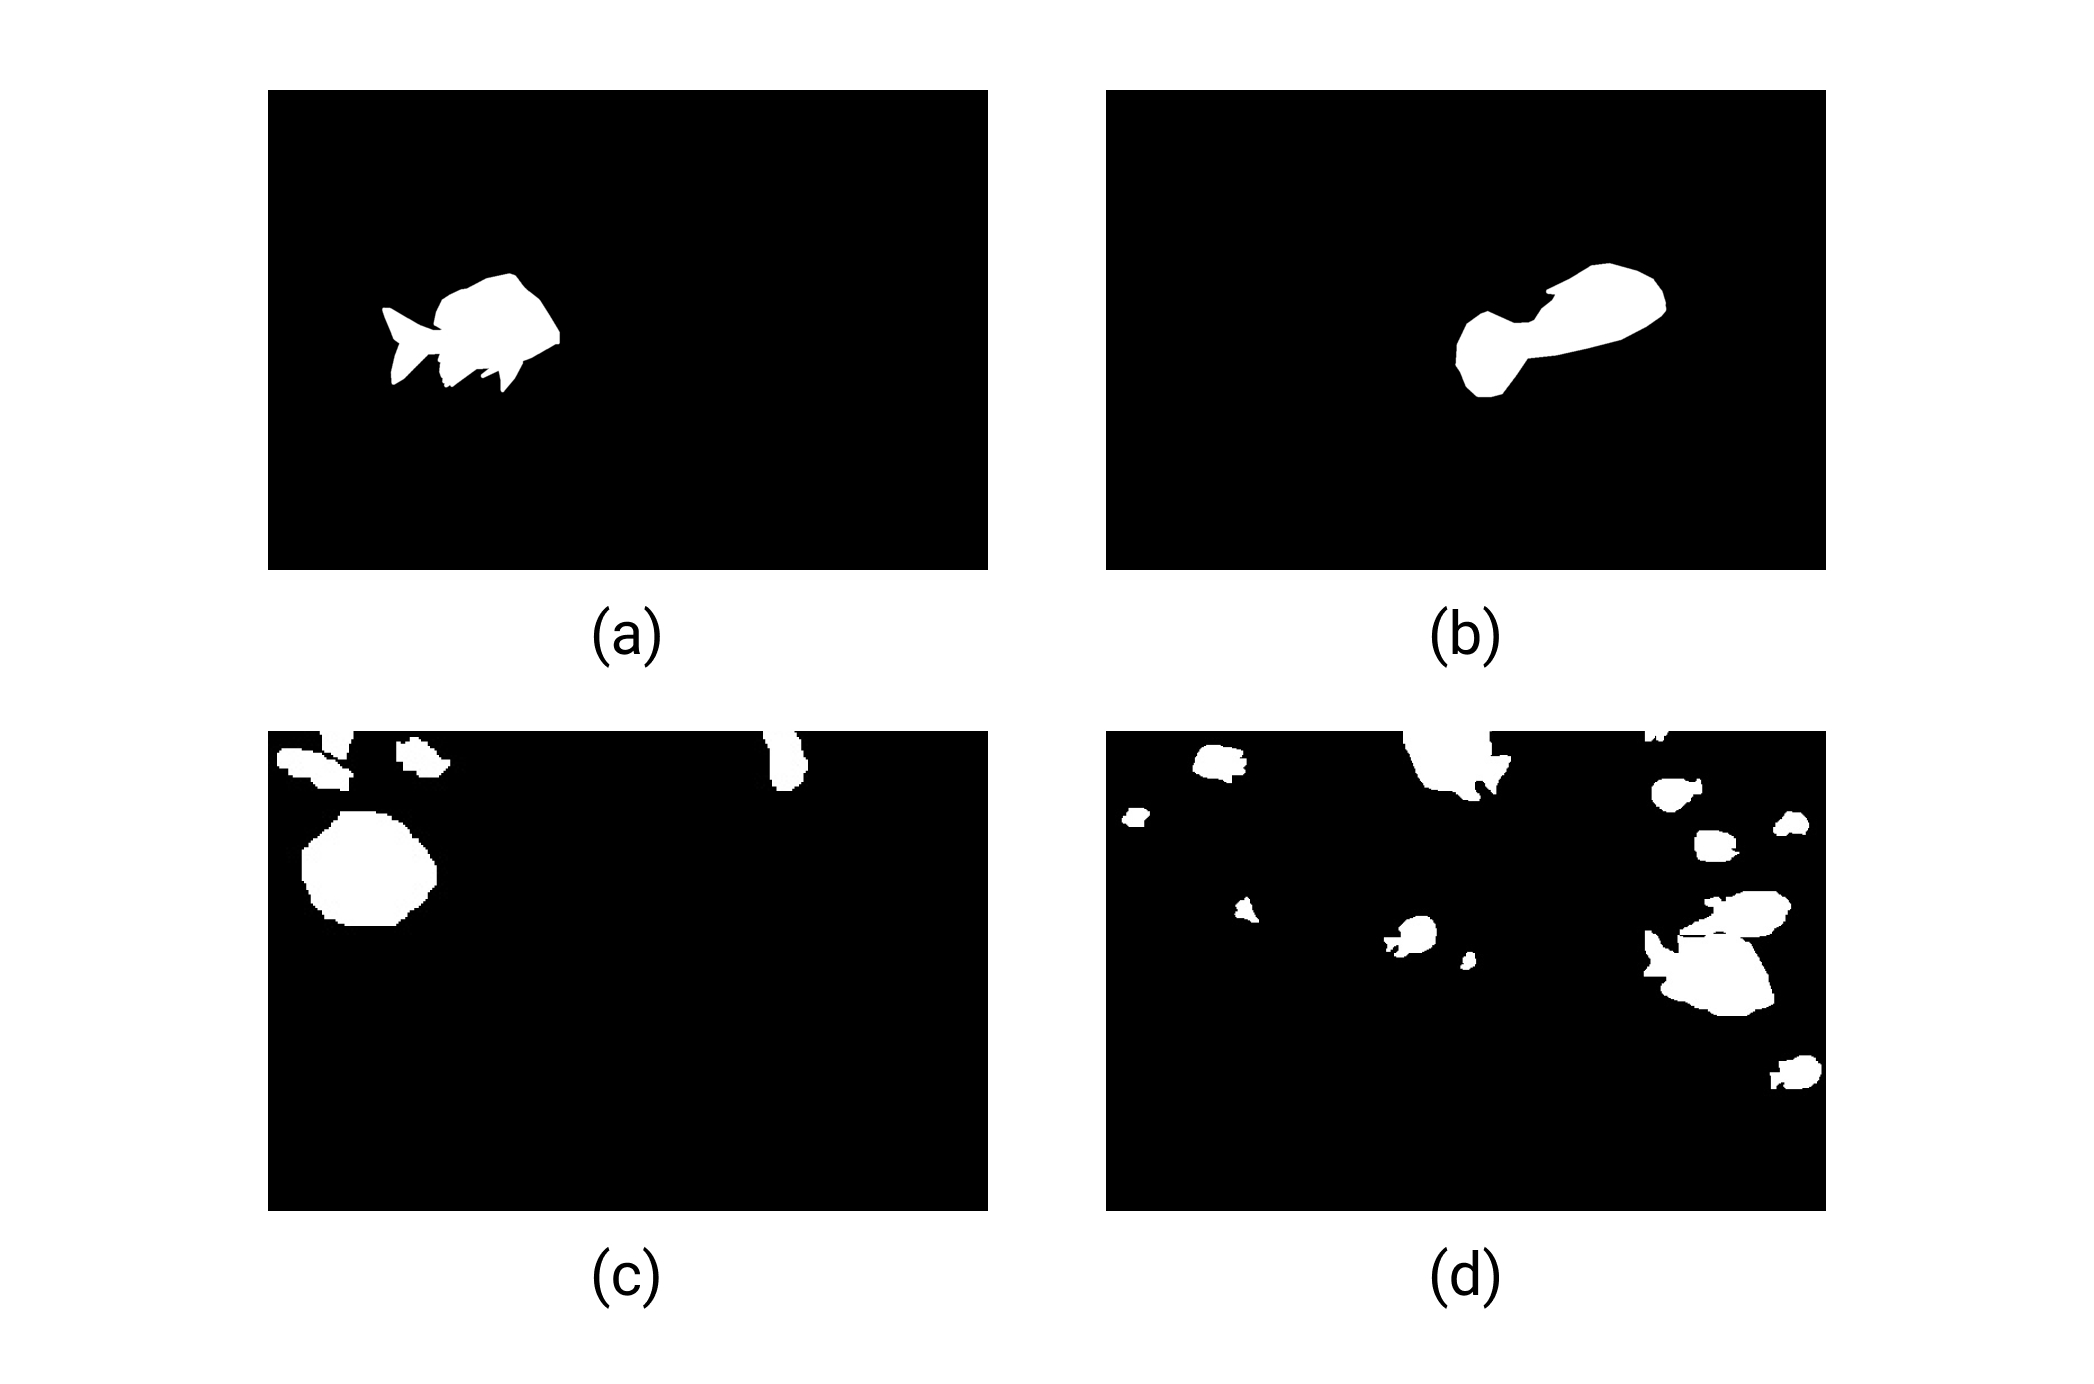
\includegraphics[width=14cm]{image/sample_groundtruth.jpg}
          \caption{Sampel \textit{groundtruth} data uji video indeks (a) 9908 (b) 9866 (c) gt\textunderscore124 (d) gt\textunderscore116}
          \label{fig:sample_groundtruth}
        \end{figure}

        Tabel \ref{tab:gmm_9908} memperlihatkan hasil dari dataset video kategori objek tunggal latar belakang sederhana. Untuk kategori video tersebut, dataset yang digunakan dapat dikatakan kurang optimal. Skor performa cenderung fluktuatif dikarenakan terlalu banyak \textit{noise} yang dihasilkan, serta jumlah frame yang sedikit.

        \begin{longtblr}[
            caption = {Hasil ujicoba proses \textit{background subtraction} menggunakan GMM terhadap video indeks 9908},
            label = {tab:gmm_9908}
        ]{
            colspec={|c|c|c|c|c|},
            rowhead=1
        }
            \hline
            Frame & Citra Asli & Hasil GMM & Groundtruth & \textit{F1} \\ \hline
            120 &
            \begin{minipage}{0.24\textwidth}
                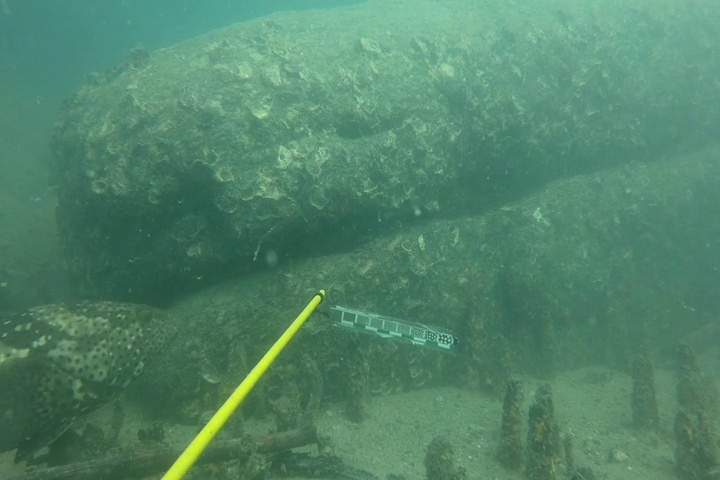
\includegraphics[width=\linewidth]{image/9908/9908_original_frame120.jpg}
            \end{minipage} &
            \begin{minipage}{0.24\textwidth}
                
\includegraphics[width=\linewidth]{image/9908/9908_gmm_frame120.jpg}
            \end{minipage} &
           \begin{minipage}{0.24\textwidth}
           	
\includegraphics[width=\linewidth]{image/9908/9908_groundtruth_120.png}
           \end{minipage} &
            58 \\ \hline
            230 &
            \begin{minipage}{0.24\textwidth}
                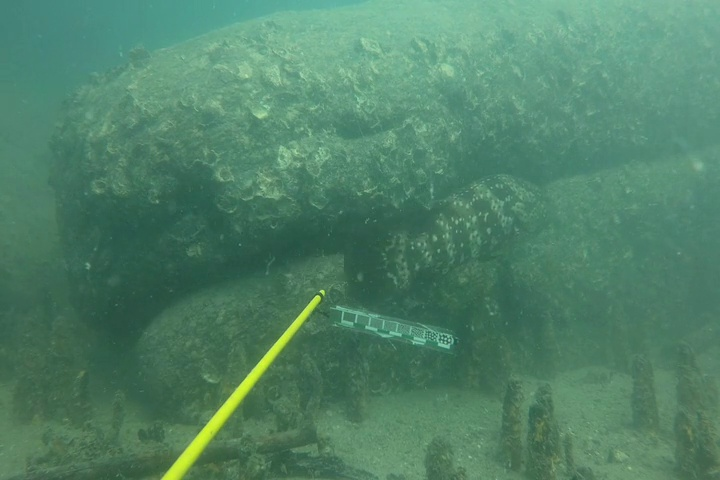
\includegraphics[width=\linewidth]{image/9908/9908_original_frame230.jpg}
            \end{minipage} &
            \begin{minipage}{0.24\textwidth}
                
\includegraphics[width=\linewidth]{image/9908/9908_gmm_frame230.jpg}
            \end{minipage} &
            \begin{minipage}{0.24\textwidth}
            	
\includegraphics[width=\linewidth]{image/9908/9908_groundtruth_230.png}
            \end{minipage} &
            31,8 \\ \hline
            290 &
            \begin{minipage}{0.24\textwidth}
                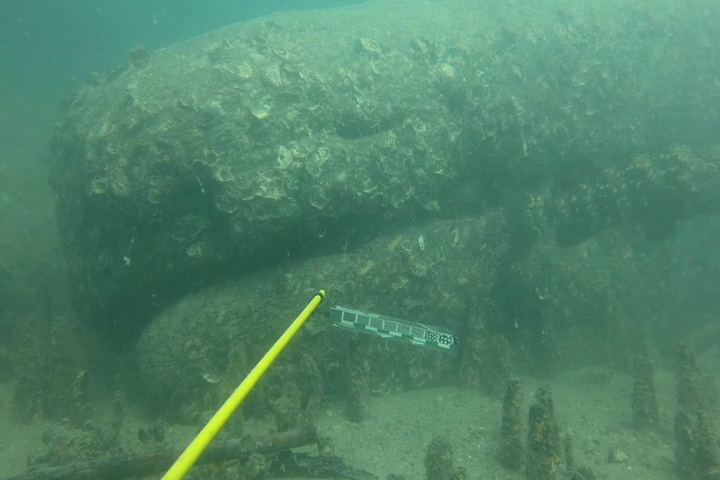
\includegraphics[width=\linewidth]{image/9908/9908_original_frame290.jpg}
            \end{minipage} &
            \begin{minipage}{0.24\textwidth}
                
\includegraphics[width=\linewidth]{image/9908/9908_gmm_frame290.jpg}
            \end{minipage} &
            \begin{minipage}{0.24\textwidth}
            	
\includegraphics[width=\linewidth]{image/9908/9908_groundtruth_290.png}
            \end{minipage} &
            58,4 \\ \hline
        \end{longtblr}
    
    	\vspace{1.5cm}

        \begin{longtblr}[
            caption = {Hasil ujicoba proses \textit{background subtraction} menggunakan GMM terhadap video indeks 9986},
            label = {tab:gmm_9986}
        ]{
            colspec={|c|c|c|c|c|c|c|},
            rowhead=1
        }
            \hline
            Frame & Citra Asli & Hasil GMM & Groundtruth & \textit{F1} \\ \hline
            509 &
            \begin{minipage}{0.24\textwidth}
                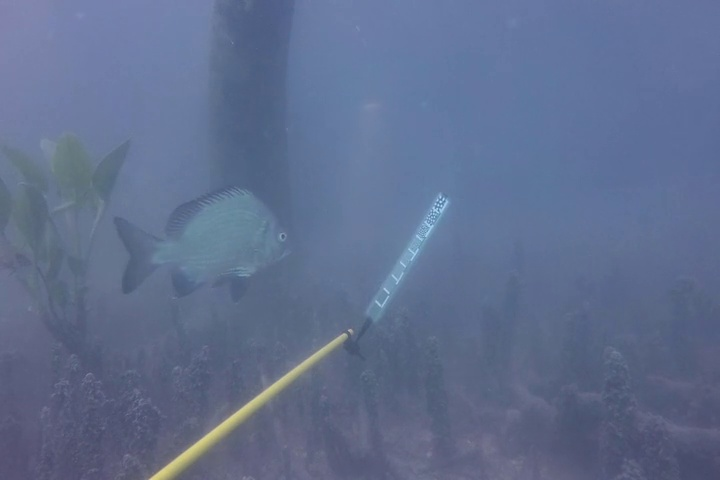
\includegraphics[width=\linewidth]{image/9866/9866_original_frame509.jpg}
            \end{minipage} &
            \begin{minipage}{0.24\textwidth}
                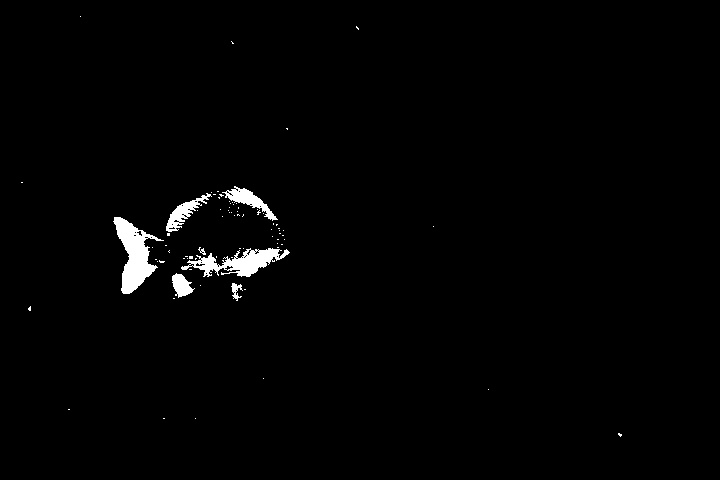
\includegraphics[width=\linewidth]{image/9866/9866_gmm_frame509.jpg}
            \end{minipage} &
           \begin{minipage}{0.24\textwidth}
           	
\includegraphics[width=\linewidth]{image/9866/9866_groundtruth_509.png}
           \end{minipage} &
            41,7 \\ \hline
            789 &
            \begin{minipage}{0.24\textwidth}
                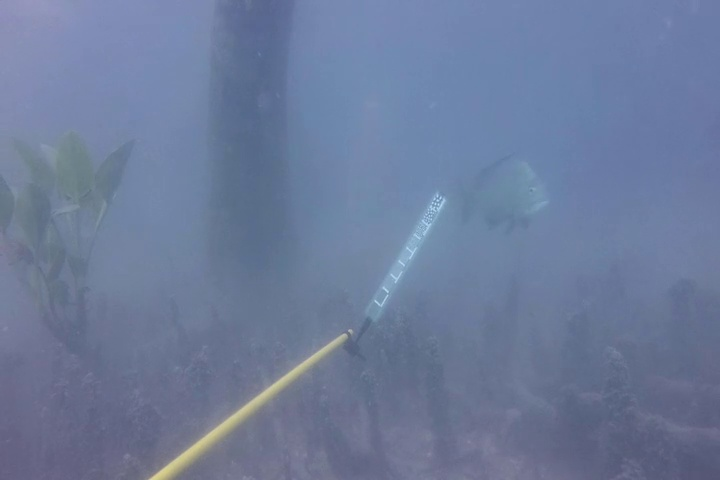
\includegraphics[width=\linewidth]{image/9866/9866_original_frame789.jpg}
            \end{minipage} &
            \begin{minipage}{0.24\textwidth}
                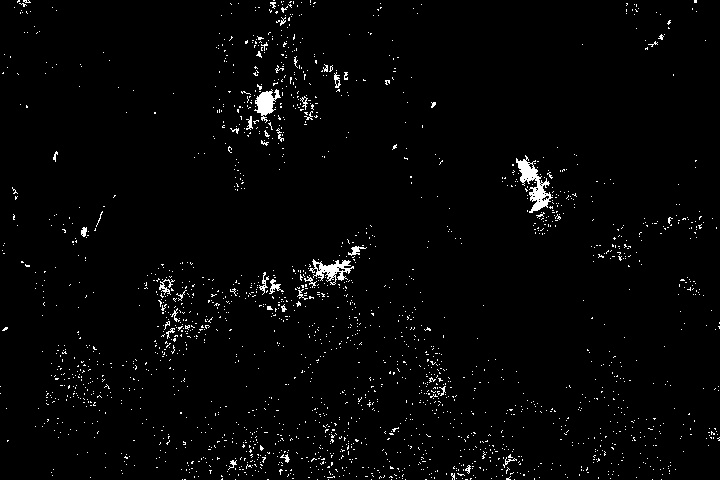
\includegraphics[width=\linewidth]{image/9866/9866_gmm_frame789.jpg}
            \end{minipage} &
            \begin{minipage}{0.24\textwidth}
            	
\includegraphics[width=\linewidth]{image/9866/9866_groundtruth_789.png}
            \end{minipage} &
            8,4 \\ \hline
            849 &
            \begin{minipage}{0.24\textwidth}
                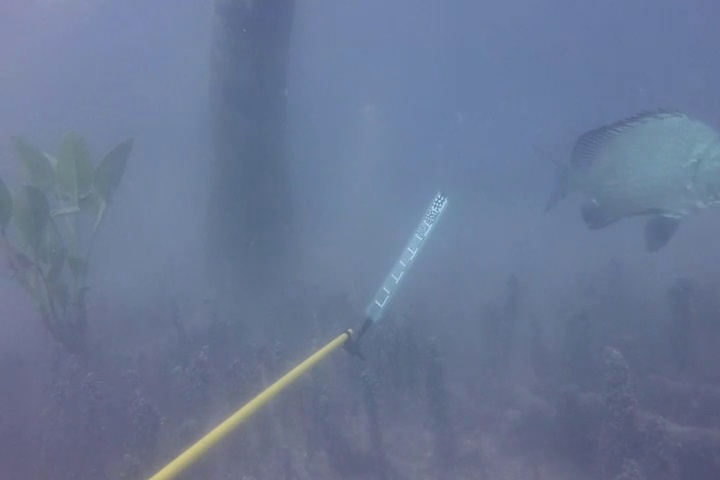
\includegraphics[width=\linewidth]{image/9866/9866_original_frame849.jpg}
            \end{minipage} &
            \begin{minipage}{0.24\textwidth}
                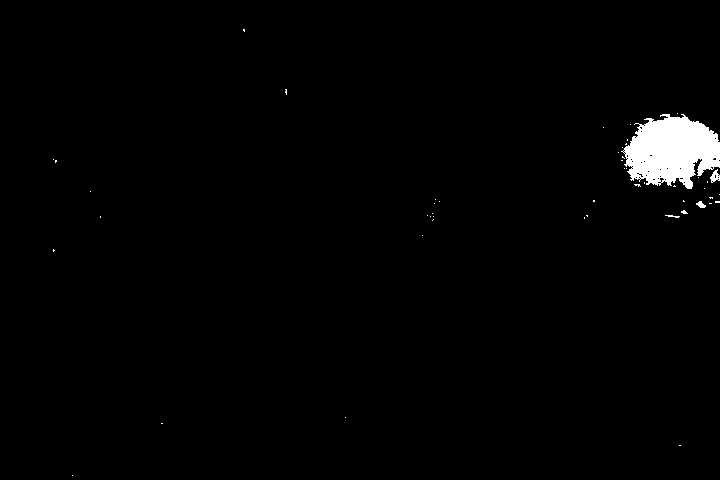
\includegraphics[width=\linewidth]{image/9866/9866_gmm_frame849.jpg}
            \end{minipage} &
            \begin{minipage}{0.24\textwidth}
            	
\includegraphics[width=\linewidth]{image/9866/9866_groundtruth_849.png}
            \end{minipage} &
            44,8 \\ \hline
        \end{longtblr}

        Tabel \ref{tab:gmm_9986} memperlihatkan hasil GMM pada video kategori kedua yaitu, objek tunggal latar belakang kompleks. Dalam pengujian, ketika terdapat \textit{burst of dynamic background} dalam waktu yang singkat (\textit{frame} 789), GMM tampak kesulitan menghasilkan keluaran yang diharapkan, beberapa objek latar belakang yang bergerak \textit{sewaktu-waktu} juga ikut terdeteksi, sehingga menghasilkan skor yang cukup buruk pada frame tersebut.

        \begin{longtblr}[
            caption = {Hasil uji coba proses \textit{background subtraction} menggunakan GMM terhadap video indeks gt\textunderscore124},
            label = {tab:gmm_124}
        ]{
            colspec={|c|c|c|c|c|c|c|},
            rowhead=1
        }
            \hline
            Frame & Citra Asli & Hasil GMM & Groundtruth & \textit{F1} \\ \hline
            705 &
            \begin{minipage}{0.24\textwidth}
                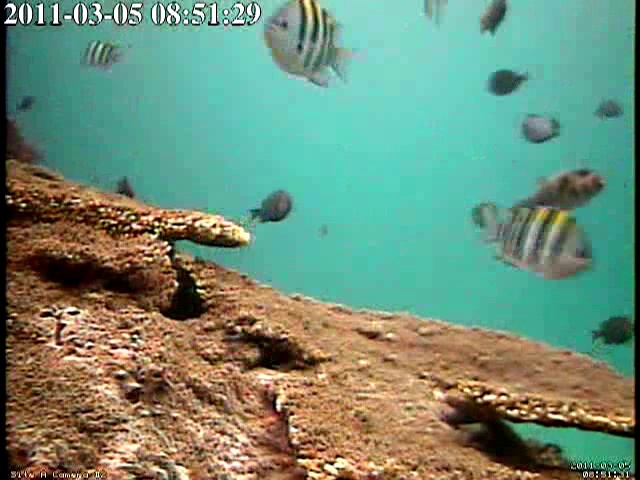
\includegraphics[width=\linewidth]{image/gt_124/gt_124_original_frame705.jpg}
            \end{minipage} &
            \begin{minipage}{0.24\textwidth}
                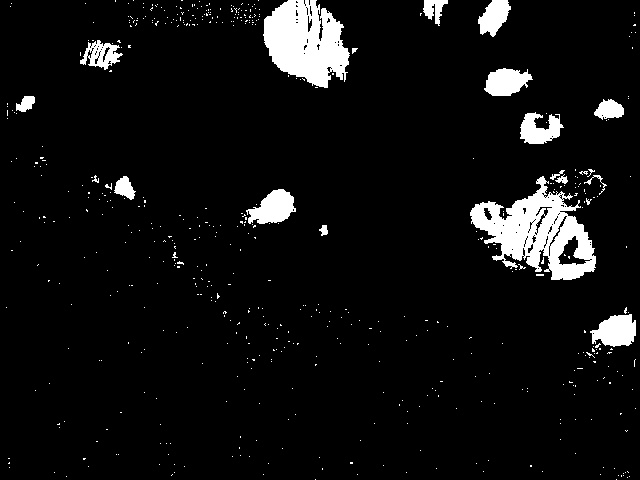
\includegraphics[width=\linewidth]{image/gt_124/gt_124_gmm_frame705.jpg}
            \end{minipage} &
            \begin{minipage}{0.24\textwidth}
            	
\includegraphics[width=\linewidth]{image/gt_124/gt_124_groundtruth_705.jpg}
            \end{minipage} &
            68,5 \\ \hline
            1173 &
            \begin{minipage}{0.24\textwidth}
                \includegraphics[width=\linewidth]{image/gt_124/gt_124_original_frame1173.jpg}
            \end{minipage} &
            \begin{minipage}{0.24\textwidth}
                \includegraphics[width=\linewidth]{image/gt_124/gt_124_gmm_frame1173.jpg}
            \end{minipage} &
            \begin{minipage}{0.24\textwidth}
            	\includegraphics[width=\linewidth]{image/gt_124/gt_124_groundtruth_1173.jpg}
            \end{minipage} &
            80 \\ \hline
            1191 &
            \begin{minipage}{0.24\textwidth}
                \includegraphics[width=\linewidth]{image/gt_124/gt_124_original_frame1191.jpg}
            \end{minipage} &
            \begin{minipage}{0.24\textwidth}
                \includegraphics[width=\linewidth]{image/gt_124/gt_124_gmm_frame1191.jpg}
            \end{minipage} &
           \begin{minipage}{0.24\textwidth}
           	\includegraphics[width=\linewidth]{image/gt_124/gt_124_groundtruth_1191.jpg}
           \end{minipage} &
            67,1 \\ \hline
        \end{longtblr}

        Selanjutnya, GMM dapat menghasilkan keluaran yang cukup baik jika latar belakang video termasuk ke dalam kategori sederhana. Hal ini dapat terlihat pada Tabel \ref{tab:gmm_124} dimana skor tertinggi berada di angka $80\%$, dengan menghasilkan sedikit \textit{noise} yang nantinya akan dieliminasi lebih baik lagi oleh Operasi Morfologi.
        
        Berbeda dengan kasus video indeks gt\textunderscore124, latar belakang pada video indeks gt\textunderscore116 (Tabel \ref{tab:gmm_116}) merupakan latar belakang yang \textit{sangat} dinamis dan kompleks. Dari hasil pengujian, walaupun rata-rata skor yang dihasilkan adalah $58\%$, GMM tampak gagal dalam mengesktrak objek ikan secara keseluruhan. Dikarenakan masih terdapat banyak \textit{noise} latar belakang yang ikut terdeteksi sebagai objek bergerak. Hal ini akan berpengaruh terhadap jumlah objek serta jumlah \textit{track} pada metode-metode selanjutnya, yaitu \textit{Contour Tracing} dan \textit{Kalman Filter}.

        \begin{longtblr}[
            caption = {Hasil uji coba proses \textit{background subtraction} menggunakan GMM terhadap video indeks gt\textunderscore116},
            label = {tab:gmm_116}
        ]{
            colspec={|c|c|c|c|c|c|c|},
            rowhead=1
        }
            \hline
            Frame & Citra Asli & Hasil GMM & Groundtruth & \textit{F1} \\ \hline
            803 &
            \begin{minipage}{0.24\textwidth}
                \includegraphics[width=\linewidth]{image/gt_116/gt_116_original_frame803.jpg}
            \end{minipage} &
            \begin{minipage}{0.24\textwidth}
                \includegraphics[width=\linewidth]{image/gt_116/gt_116_gmm_frame803.jpg}
            \end{minipage} &
            \begin{minipage}{0.24\textwidth}
            	\includegraphics[width=\linewidth]{image/gt_116/gt_116_groundtruth_803.jpg}
            \end{minipage} &
            43,5 \\ \hline
            859 &
            \begin{minipage}{0.24\textwidth}
                \includegraphics[width=\linewidth]{image/gt_116/gt_116_original_frame859.jpg}
            \end{minipage} &
            \begin{minipage}{0.24\textwidth}
                \includegraphics[width=\linewidth]{image/gt_116/gt_116_gmm_frame859.jpg}
            \end{minipage} &
           \begin{minipage}{0.24\textwidth}
           	\includegraphics[width=\linewidth]{image/gt_116/gt_116_groundtruth_859.jpg}
           \end{minipage} &
            55,2 \\ \hline
            1167 &
            \begin{minipage}{0.24\textwidth}
                \includegraphics[width=\linewidth]{image/gt_116/gt_116_original_frame1167.jpg}
            \end{minipage} &
            \begin{minipage}{0.24\textwidth}
                \includegraphics[width=\linewidth]{image/gt_116/gt_116_gmm_frame1167.jpg}
            \end{minipage} &
            \begin{minipage}{0.24\textwidth}
            	\includegraphics[width=\linewidth]{image/gt_116/gt_116_groundtruth_1167.jpg}
            \end{minipage} &
            50,7 \\ \hline
        \end{longtblr}

        \vspace{-0.5cm}
        \begin{figure}[H]
        \centering
          \singlespacing
          \captionsetup{justification=centering,margin=0.5cm}
          \includegraphics[width=14cm]{image/CodeSnap/gmm.png}
          \caption{Potongan sampel kode Background Subtraction yang dibantu oleh GMM}
          \label{fig:Potongan sampel kode gmm}
        \end{figure}
    
    	\begin{longtblr}[
    		caption = {Skor \textit{Accuracy}, \textit{Recall}, \textit{Precision}, dan \textit{F1} pada metode \textit{Background Subtraction} menggunakan GMM},
    		label = {tab:gmm_skor}
    		]{
    			colspec={|c|c|c|c|c|c|},
    			rowhead=1
    		}
    		\hline
    		Indeks & Frame & \textit{Accuracy} & \textit{Recall} & \textit{Precision} & \textit{F1 Score} \\ \hline
    		9908 &
    		120 &
    		96 &
    		50,3 &
    		68,6 &
    		58 \\ \hline
    		9908 &
    		230 &
    		94,8 &
    		31,9 &
    		31,7 &
    		31,8 \\ \hline
    		9908 &
    		290 &
    		97,2 &
    	    46,9 &
    		77,4 &
    		58,4 \\ \hline
    		9866 &
    		509 &
    		97,5 &
    		27 &
    		91,4 &
    		41,7 \\ \hline
    		9866 &
    		789 &
    		97,6 &
    		9 &
    		7 &
    		8 \\ \hline
    		9866 &
    		849 &
    		96,9 &
    		28,9 &
    		99,4 &
    		44,8 \\ \hline
    		gt\textunderscore124 &
    		705 &
    		96,5 &
    		60,3 &
    		79,2 &
    		68,5 \\ \hline
    		gt\textunderscore124 &
    		1173 &
    		97,4 &
    		79,9 &
    		80,1 &
    		80 \\ \hline
    		gt\textunderscore124 &
    		1191 &
    		95,4 &
    		59,1 &
    		77,7 &
    		67,1 \\ \hline
    		gt\textunderscore116 &
    		803 &
    		94,9 &
    		49,7 &
    		38,6 &
    		43,5 \\ \hline
    		gt\textunderscore116 &
    		859 &
    		94,1 &
    		55,8 &
    		54,9 &
    		55,2 \\ \hline
    		gt\textunderscore116 &
    		1167 &
    		93,6 &
    		49,3 &
    		52,3 &
    		50,7 \\ \hline
    	\end{longtblr}
    
    	Secara teori, GMM seharusnya dapat menghasilkan keluaran yang lebih baik seiring dengan bertambahnya \textit{frame} yang diolah oleh sistem. Dikarenakan proses \textit{training} model latar belakang oleh GMM dapat memanfaatkan jumlah dataset yang lebih banyak. Akan tetapi pada praktiknya, banyak juga faktor yang dapat membuat keluaran metode ini kurang baik. Hasil yang diharapkan adalah skor \textit{Precision} dan \textit{Recall} yang mendekati satu, dimana \textit{Precision} merepresentasikan seberapa besar kasus positif (piksel latar depan) yang benar dari seluruh prediksi positif, dan \textit{Recall} merepresentasikan seberapa besar kasus positif yang benar dari seluruh kasus positif di dataset.
    	
    	Jika dilihat pada Tabel \ref{tab:gmm_skor}, secara garis besar skor GMM cenderung fluktuatif, bahkan dalam beberapa kasus GMM tampak gagal dalam mengekstraksi objek ikan. Contohnya ada pada video indeks 9866 \textit{frame} 789, \textit{F1 Score} menyentuh angka yang sangat rendah, yaitu $8\%$. Hal ini dikarenakan metode mengalami lonjakan input latar belakang dinamis yang sangat besar pada \textit{frame} tersebut. Artinya, model latar belakang yang di-\textit{generate} oleh GMM gagal dalam mengklasifikasikan piksel \textit{frame} ke dalam kelasnya masing-masing.
    	
    	Hal lain yang dapat disimpulkan adalah pada video indeks 9908 dan gt\textunderscore124, dimana kedua dataset tersebut merupakan dataset dengan kategori latar belakang sederhana, menghasilkan rata-rata skor yang lebih tinggi dari pada video indeks 9866 dan gt\textunderscore116, yang merupakan video dengan kategori latar belakang kompleks. Hasil ini seperti yang diharapkan penulis, GMM akan megnhasilkan keluaran yang lebih baik jika sedari awal \textit{noise} yang ada pada masukkan sistem sudah sangat \textit{minim}. Walaupn salah satu fungsi dari GMM itu sendiri adalah mengeliminasi \textit{noise} yang berulang (seperti dahan pohon yang berayun dan iluminasi), akan tetapi jika \textit{noise} itu sendiri sudah tidak ada pada video masukkan tentu hal ini akan berpengaruh terhadap meningkatnya skor yang dihasilkan.
    	
    	\begin{equation}\label{eq:3.5}
    		Precision = \frac{TP}{TP + FP} = \frac{\textit{N. of Correctly Predicted Positive Instances}}{\textit{N. of Total Positive Predictions We Made}}
    	\end{equation}
    
    	\begin{equation}\label{eq:3.5}
	    	Recall = \frac{TP}{TP + FN} = \frac{\textit{N. of Correctly Predicted Positive Instances}}{\textit{N. of Total Positive Instances in the Dataset}}
    	\end{equation}
    
    \vspace{2cm}
        
	\section{Operasi Morfologi}
		Selanjutnya, citra melewati proses eliminasi \textit{noise} menggunakan Operasi Morfologi. Dalam pengujian tahap ini, percobaan dilakukan dengan beberapa nilai \textit{structuring element / kernel} Operasi Morfologi yang berbeda-beda.
  
        \begin{longtblr}[
            caption = {Hasil uji coba proses \textit{background subtraction} menggunakan GMM yang disempurnakan oleh Operasi Morfologi},
            label = {tab:gmm_morph_9908}
        ]{
            colspec={|Q[c,m,1.2cm]|c|c|c|c|},
            rowhead=2
        }
            \hline
            \SetCell[r=2]{} Id / Frame & 
            \SetCell[r=2]{} Hasil GMM &
            \SetCell[c=3]{}{Kernel} \\ \cline{3-5}
            & & $3 \times 9$ & $5 \times 11$ & $7 \times 13$ \\ 
            \hline
            9908 / 120 &
            \begin{minipage}{0.19\textwidth}
                \includegraphics[width=\linewidth]{image/9908/9908_gmm_frame120.jpg}
            \end{minipage} & 
            \begin{minipage}{0.19\textwidth}
                \includegraphics[width=\linewidth]{image/9908/9908_dilated_3x9_frame120.jpg}
            \end{minipage} &
            \begin{minipage}{0.19\textwidth}
                \includegraphics[width=\linewidth]{image/9908/9908_dilated_5x11_frame120.jpg}
            \end{minipage} & 
            \begin{minipage}{0.19\textwidth}
                \includegraphics[width=\linewidth]{image/9908/9908_dilated_7x13_frame120.jpg}
            \end{minipage} \\
            \hline
            9908 / 230 &
            \begin{minipage}{0.19\textwidth}
                \includegraphics[width=\linewidth]{image/9908/9908_gmm_frame230.jpg}
            \end{minipage} & 
            \begin{minipage}{0.19\textwidth}
                \includegraphics[width=\linewidth]{image/9908/9908_dilated_3x9_frame230.jpg}
            \end{minipage} &
            \begin{minipage}{0.19\textwidth}
                \includegraphics[width=\linewidth]{image/9908/9908_dilated_5x11_frame230.jpg}
            \end{minipage} & 
            \begin{minipage}{0.19\textwidth}
                \includegraphics[width=\linewidth]{image/9908/9908_dilated_7x13_frame230.jpg}
            \end{minipage} \\
            \hline
            9908 / 290 &
            \begin{minipage}{0.19\textwidth}
                \includegraphics[width=\linewidth]{image/9908/9908_gmm_frame290.jpg}
            \end{minipage} & 
            \begin{minipage}{0.19\textwidth}
                \includegraphics[width=\linewidth]{image/9908/9908_dilated_3x9_frame290.jpg}
            \end{minipage} &
            \begin{minipage}{0.19\textwidth}
                \includegraphics[width=\linewidth]{image/9908/9908_dilated_5x11_frame290.jpg}
            \end{minipage} & 
            \begin{minipage}{0.19\textwidth}
                \includegraphics[width=\linewidth]{image/9908/9908_dilated_7x13_frame290.jpg}
            \end{minipage} \\
            \hline
            9866 / 509 &
            \begin{minipage}{0.19\textwidth}
                \includegraphics[width=\linewidth]{image/9866/9866_gmm_frame509.jpg}
            \end{minipage} & 
            \begin{minipage}{0.19\textwidth}
                \includegraphics[width=\linewidth]{image/9866/9866_dilated_3x9_frame509.jpg}
            \end{minipage} &
            \begin{minipage}{0.19\textwidth}
                \includegraphics[width=\linewidth]{image/9866/9866_dilated_5x11_frame509.jpg}
            \end{minipage} & 
            \begin{minipage}{0.19\textwidth}
                \includegraphics[width=\linewidth]{image/9866/9866_dilated_7x13_frame509.jpg}
            \end{minipage} \\
            \hline
            9866 / 789 &
            \begin{minipage}{0.19\textwidth}
                \includegraphics[width=\linewidth]{image/9866/9866_gmm_frame789.jpg}
            \end{minipage} & 
            \begin{minipage}{0.19\textwidth}
                \includegraphics[width=\linewidth]{image/9866/9866_dilated_3x9_frame789.jpg}
            \end{minipage} &
            \begin{minipage}{0.19\textwidth}
                \includegraphics[width=\linewidth]{image/9866/9866_dilated_5x11_frame789.jpg}
            \end{minipage} & 
            \begin{minipage}{0.19\textwidth}
                \includegraphics[width=\linewidth]{image/9866/9866_dilated_7x13_frame789.jpg}
            \end{minipage} \\
            \hline
            9866 / 849 &
            \begin{minipage}{0.19\textwidth}
                \includegraphics[width=\linewidth]{image/9866/9866_gmm_frame849.jpg}
            \end{minipage} & 
            \begin{minipage}{0.19\textwidth}
                \includegraphics[width=\linewidth]{image/9866/9866_dilated_3x9_frame849.jpg}
            \end{minipage} &
            \begin{minipage}{0.19\textwidth}
                \includegraphics[width=\linewidth]{image/9866/9866_dilated_5x11_frame849.jpg}
            \end{minipage} & 
            \begin{minipage}{0.19\textwidth}
                \includegraphics[width=\linewidth]{image/9866/9866_dilated_7x13_frame849.jpg}
            \end{minipage} \\
            \hline
            gt\textunderscore124 / 705 &
            \begin{minipage}{0.19\textwidth}
                \includegraphics[width=\linewidth]{image/gt_124/gt_124_gmm_frame705.jpg}
            \end{minipage} & 
            \begin{minipage}{0.19\textwidth}
                \includegraphics[width=\linewidth]{image/gt_124/gt_124_dilated_3x9_frame705.jpg}
            \end{minipage} &
            \begin{minipage}{0.19\textwidth}
                \includegraphics[width=\linewidth]{image/gt_124/gt_124_dilated_5x11_frame705.jpg}
            \end{minipage} & 
            \begin{minipage}{0.19\textwidth}
                \includegraphics[width=\linewidth]{image/gt_124/gt_124_dilated_7x13_frame705.jpg}
            \end{minipage} \\
            \hline
            gt\textunderscore124 / 1173 &
            \begin{minipage}{0.19\textwidth}
                \includegraphics[width=\linewidth]{image/gt_124/gt_124_gmm_frame1173.jpg}
            \end{minipage} & 
            \begin{minipage}{0.19\textwidth}
                \includegraphics[width=\linewidth]{image/gt_124/gt_124_dilated_3x9_frame1173.jpg}
            \end{minipage} &
            \begin{minipage}{0.19\textwidth}
                \includegraphics[width=\linewidth]{image/gt_124/gt_124_dilated_5x11_frame1173.jpg}
            \end{minipage} & 
            \begin{minipage}{0.19\textwidth}
                \includegraphics[width=\linewidth]{image/gt_124/gt_124_dilated_7x13_frame1173.jpg}
            \end{minipage} \\
            \hline
            gt\textunderscore124 / 1191 &
            \begin{minipage}{0.19\textwidth}
                \includegraphics[width=\linewidth]{image/gt_124/gt_124_gmm_frame1191.jpg}
            \end{minipage} & 
            \begin{minipage}{0.19\textwidth}
                \includegraphics[width=\linewidth]{image/gt_124/gt_124_dilated_3x9_frame1191.jpg}
            \end{minipage} &
            \begin{minipage}{0.19\textwidth}
                \includegraphics[width=\linewidth]{image/gt_124/gt_124_dilated_5x11_frame1191.jpg}
            \end{minipage} & 
            \begin{minipage}{0.19\textwidth}
                \includegraphics[width=\linewidth]{image/gt_124/gt_124_dilated_7x13_frame1191.jpg}
            \end{minipage} \\
            \hline
            gt\textunderscore116 / 803 &
            \begin{minipage}{0.19\textwidth}
                \includegraphics[width=\linewidth]{image/gt_116/gt_116_gmm_frame803.jpg}
            \end{minipage} & 
            \begin{minipage}{0.19\textwidth}
                \includegraphics[width=\linewidth]{image/gt_116/gt_116_dilated_3x9_frame803.jpg}
            \end{minipage} &
            \begin{minipage}{0.19\textwidth}
                \includegraphics[width=\linewidth]{image/gt_116/gt_116_dilated_5x11_frame803.jpg}
            \end{minipage} & 
            \begin{minipage}{0.19\textwidth}
                \includegraphics[width=\linewidth]{image/gt_116/gt_116_dilated_7x13_frame803.jpg}
            \end{minipage} \\
            \hline
            gt\textunderscore116 / 859 &
            \begin{minipage}{0.19\textwidth}
                \includegraphics[width=\linewidth]{image/gt_116/gt_116_gmm_frame859.jpg}
            \end{minipage} & 
            \begin{minipage}{0.19\textwidth}
                \includegraphics[width=\linewidth]{image/gt_116/gt_116_dilated_3x9_frame859.jpg}
            \end{minipage} &
            \begin{minipage}{0.19\textwidth}
                \includegraphics[width=\linewidth]{image/gt_116/gt_116_dilated_5x11_frame859.jpg}
            \end{minipage} & 
            \begin{minipage}{0.19\textwidth}
                \includegraphics[width=\linewidth]{image/gt_116/gt_116_dilated_7x13_frame859.jpg}
            \end{minipage} \\
            \hline
            gt\textunderscore116 / 1167 &
            \begin{minipage}{0.19\textwidth}
                \includegraphics[width=\linewidth]{image/gt_116/gt_116_gmm_frame1167.jpg}
            \end{minipage} & 
            \begin{minipage}{0.19\textwidth}
                \includegraphics[width=\linewidth]{image/gt_116/gt_116_dilated_3x9_frame1167.jpg}
            \end{minipage} &
            \begin{minipage}{0.19\textwidth}
                \includegraphics[width=\linewidth]{image/gt_116/gt_116_dilated_5x11_frame1167.jpg}
            \end{minipage} & 
            \begin{minipage}{0.19\textwidth}
                \includegraphics[width=\linewidth]{image/gt_116/gt_116_dilated_7x13_frame1167.jpg}
            \end{minipage} \\
            \hline
        \end{longtblr}
    
        Digunakan $3$ parameter \textit{structuring element / kernel} (Operasi Morfologi) untuk masing-masing sampel \textit{frame}. Proses ini menyempurnakan keluaran metode GMM dengan menghapus \textit{noise (noise removal)} secara lebih \textbf{agresif} dan menghasilkan citra biner yang diharapkan bersih dari \textit{noise}. Fokus dari Operasi Morfologi adalah menghapus \textit{noise} sebanyak-banyaknya. Jika dilihat pada Tabel \ref{tab:skor_morph}, skor \textit{metric} cenderung mengalami penurunan seiring dengan semakin besarnya ukuran \textit{kernel} yang digunakan. Hal ini dikarenakan ukuran \textit{kernel} yang lebih besar akan mengikis piksel lebih banyak dari pada ukuran \textit{kernel} yang lebih kecil. Penentuan besaran ukuran \textit{kernel} perlu mempertimbangkan rata-rata ukuran objek yang ingin dilacak untuk meminimalisir piksel objek tereliminasi, atau bahkan dalam kasus terburuk objek tersebut hilang dari \textit{frame}.

        \begin{longtblr}[
            caption = {Skor \textit{Accuracy, Recall, Precision, dan F1} Operasi Morfologi},
            label = {tab:skor_morph}
        ]{
            colspec={|c|c|c|Q[c,m,1.75cm]|Q[c,m,1.75cm]|Q[c,m,1.75cm]|Q[c,m,1.75cm]|},
            rowhead=1
        }
            \hline
            Indeks & Frame & \textit{Kernel} & \textit{Accuracy} & \textit{Recall} & \textit{Precision} & \textit{F1} \\ \hline
            \SetCell[r=3]{} 9908 & \SetCell[r=3]{} 120 & $3 \times 9$ & 96,8 & 78,6 & 68,3 & 73,1 \\ \cline{3-7}
            & & $5 \times 11$ & 97,1 & 68 & 76,1 & 71,8 \\ \cline{3-7}
            & & $7 \times 13$ & 96,8 & 58 & 77,1 & 66,2 \\
            \hline
            \SetCell[r=3]{} 9908 & \SetCell[r=3]{} 230 & $3 \times 9$ & 94,5 & 64,1 & 36,9 & 46,9 \\ \cline{3-7}
            & & $5 \times 11$ & 94,6 & 38,2 & 32,2 & 35 \\ \cline{3-7}
            & & $7 \times 13$ & 94,4 & 12,2 & 16,6 & 14,1 \\
            \hline
            \SetCell[r=3]{} 9908 & \SetCell[r=3]{} 290 & $3 \times 9$ & 97,8 & 70,2 & 76,2 & 73,1 \\ \cline{3-7}
            & & $5 \times 11$ & 97,7 & 57,7 & 88,4 & 69,8 \\ \cline{3-7}
            & & $7 \times 13$ & 97,8 & 51,6 & 92,9 & 66,4 \\
            \hline
            \SetCell[r=3]{} 9866 & \SetCell[r=3]{} 509 & $3 \times 9$ & 97,7 & 44 & 76,8 & 55,9 \\ \cline{3-7}
            & & $5 \times 11$ & 97,5 & 37,4 & 78,1 & 50,5 \\ \cline{3-7}
            & & $7 \times 13$ & 97,4 & 32,7 & 78,5 & 46,2 \\
            \hline
            \SetCell[r=3]{} 9866 & \SetCell[r=3]{} 789 & $3 \times 9$ & 98,1 & 17,5 & 19 & 18,2 \\ \cline{3-7}
            & & $5 \times 11$ & 98,6 & 13,7 & 32,9 & 19,4 \\ \cline{3-7}
            & & $7 \times 13$ & 98,7 & 10,8 & 34,9 & 16,5 \\
            \hline
            \SetCell[r=3]{} 9866 & \SetCell[r=3]{} 849 & $3 \times 9$ & 97,3 & 39,8 & 99 & 56,8 \\ \cline{3-7}
            & & $5 \times 11$ & 97,2 & 36,6 & 99,5 & 53,5 \\ \cline{3-7}
            & & $7 \times 13$ & 97,1 & 34,1 & 99,5 & 50,9 \\
            \hline
            \SetCell[r=1]{} gt\textunderscore124 & \SetCell[r=1]{} 705 & $3 \times 9$ & 96,8 & 86,3 & 69,8  & 77,2 \\ \cline{3-7}
            & & $5 \times 11$ & 96,6 & 80,5 & 70,5 & 75,2 \\ \cline{3-7}
            & & $7 \times 13$ & 96,5 & 74,4 & 71,5 & 72,9 \\
            \hline
            \SetCell[r=3]{} gt\textunderscore124 & \SetCell[r=3]{} 1173 & $3 \times 9$ & 96,5 & 94,6 & 66 & 77,8 \\ \cline{3-7}
            & & $5 \times 11$ & 97,1 & 93 & 71 & 80 \\ \cline{3-7}
            & & $7 \times 13$ & 97,3 & 89,2 & 74,8 & 81,4 \\
            \hline
            \SetCell[r=3]{} gt\textunderscore124 & \SetCell[r=3]{} 1191 & $3 \times 9$ & 96,3 & 90,9 & 70,5 & 79,4 \\ \cline{3-7}
            & & $5 \times 11$ & 96,6 & 81,7 & 76,1 & 78,8 \\ \cline{3-7}
            & & $7 \times 13$ & 96,2 & 71,4 & 77,74 & 74,3 \\
            \hline
            \SetCell[r=3]{} gt\textunderscore116 & \SetCell[r=3]{} 803 & $3 \times 9$ & 95 & 85,1 & 43,3 & 57,4 \\ \cline{3-7}
            & & $5 \times 11$ & 96,1 & 76,8 & 50,7 & 61,1 \\ \cline{3-7}
            & & $7 \times 13$ & 96,8 & 65,3 & 59,6 & 62,3 \\
            \hline
            \SetCell[r=3]{} gt\textunderscore116 & \SetCell[r=3]{} 859 & $3 \times 9$ & 95,2 & 89,7 & 58,1 & 70,5 \\ \cline{3-7}
            & & $5 \times 11$ & 96, & 72,6 & 69,3 & 70,9 \\ \cline{3-7}
            & & $7 \times 13$ & 96,2 & 58,5 & 77,2 & 66,6 \\
            \hline
            \SetCell[r=3]{} gt\textunderscore116 & \SetCell[r=3]{} 1167 & $3 \times 9$ & 94,8 & 85, & 57,6 & 68,7 \\ \cline{3-7}
            & & $5 \times 11$ & 96,2 & 72,9 & 71,1 & 72 \\ \cline{3-7}
            & & $7 \times 13$ & 96 & 58,5 & 76 & 66 \\
            \hline
            
        \end{longtblr}

        Penentuan 2 besaran ukuran \textit{kernel} yang digunakan, juga mempertimbangkan \textit{trade-off} yang dihasilkan dari masing-masing parameter tersebut. Semakin besar ukuran \textit{kernel}, semakin sedikit \textit{noise} yang tampak, akan tetapi semakin banyak juga informasi yang hilang (piksel objek). Hal ini berdampak pada ukuran serta bentuk objek yang juga ikut menyusut. Sebaliknya, semakin kecil ukuran \textit{kernel} yang digunakan, maka semakin banyak informasi (piksel objek) yang dapat dipertahankan, namun semakin banyak juga \textit{noise} yang tampak. Hasil skor keluaran Operasi Morfologi dapat dilihat pada Tabel \ref{tab:skor_morph}. 
        
        \vspace{-0.5cm}
        \begin{figure}[H]
        \centering
          \singlespacing
          \captionsetup{justification=centering,margin=0.5cm}
          \includegraphics[width=10cm]{image/CodeSnap/morph.png}
          \caption{Potongan sampel kode \textit{Background Subtraction} dan Operasi Morfologi}
          \label{fig:code_gmm_morph}
        \end{figure}
    
    	Dari ujicoba di atas, dapat disimpulkan bahwa secara visual metode ini melaksanakan tugasnya dengan baik, yaitu mengeliminasi \textit{noise} dengan lebih agresif. Pada setiap \textit{frame} uji Tabel \ref{tab:gmm_morph_9908}, \textit{salt and peper noise} dapat dieliminasi dengan baik untuk semua ukuran \textit{structuring element} yang digunakan. Poin penting lain yang dapat diobservasi adalah skor metode yang tampak menurun seiring dengan besarnya ukuran \textit{structuring element} yang digunakan (Tabel \ref{tab:skor_morph}). Hal ini masih masuk ke dalam ekspektasi penulis dikarenakan penjelasan dari metode itu sendiri, dimana \textit{trade-off} yang dihasilkan dari semakin besarnya ukuran \textit{structuring element} yang digunakan, adalah semakin banyak piksel latar depan yang hilang, akan tetapi semakin banyak juga \textit{noise} yang tereliminasi.
    	
    	Metode ini hanya berfokus terhadap seberapa banyak \textit{noise} yang dapat dieliminasi dengan tetap mempertahankan bentuk objek sebaik mungkin. Maka dari itu, skor \textit{metric} yang semakin menurun bukan semata-mata pertanda bahwa performa sistem buruk, semua bergantung pada hasil metode selanjutnya, yaitu \textit{Contour Tracing} dan \textit{Kalman Filter} yang akan memvalidasi jumlah objek hasil deteksi, agar \textit{noise} yang dihasilkan GMM tidak ikut terhitung oleh metode tersebut.

    \section{\textit{Contour Tracing} dan \textit{Downsampling}}
        Pada uji coba CT, setiap \textit{frame} data diuji dengan skala \textit{Downsampling} yang berbeda-beda. Hal ini akan berpengaruh terhadap performa metode CT. Semakin besar skala yang digunakan, maka semakin cepat performa yang didapat, begitu juga sebaliknya. Pemilihan besaran skala \textit{Downsampling} juga tetap memperhatikan hasil \textit{bounding box} dari metode CT tersebut.
        
        \begin{longtblr}[
            caption = {Hasil uji coba metode CT yang ditingkatkan oleh \textit{Downsampling} pada video indeks 9908 dengan ukuran \textit{kernel} Operasi Morfologi 7x13},
            label = {tab:ct_downsampling_9908}
        ]{
            colspec={|c|c|c|c|c|},
            rowhead=1
        }
            \hline
            Indeks & Frame & \textit{Groundtruth} & Skala & Hasil \\ 
            \hline
            % row
            \SetCell[r=3]{} 9908 &
            \SetCell[r=3]{} 120 &
            \SetCell[r=3]{} \begin{minipage}{0.3\textwidth}
                \includegraphics[width=\linewidth]{image/9908/9908_groundtruth_120.png}
            \end{minipage} &
            $\times2$ & 
            \begin{minipage}{0.3\textwidth}
                \includegraphics[width=\linewidth]{image/9908/9908_contour_downsample_x2_m7x13_frame120.jpg}
            \end{minipage} \\ \cline{3-4}
            & & & 
            $\times4$ &
            \begin{minipage}{0.3\textwidth}
                \includegraphics[width=\linewidth]{image/9908/9908_contour_downsample_x4_m7x13_frame120.jpg}
            \end{minipage} \\ \cline{3-4}
            & & & 
            $\times8$ &
            \begin{minipage}{0.3\textwidth}
                \includegraphics[width=\linewidth]{image/9908/9908_contour_downsample_x8_m7x13_frame120.jpg}
            \end{minipage} \\ 
            \hline
            % end row
            % row
            \SetCell[r=3]{} 9908 &
            \SetCell[r=3]{} 230 &
            \SetCell[r=3]{} \begin{minipage}{0.3\textwidth}
                \includegraphics[width=\linewidth]{image/9908/9908_groundtruth_230.png}
            \end{minipage} &
            $\times2$ & 
            \begin{minipage}{0.3\textwidth}
                \includegraphics[width=\linewidth]{image/9908/9908_contour_downsample_x2_m7x13_frame230.jpg}
            \end{minipage} \\ \cline{3-4}
            & & \SetCell[r=2]{} &
            $\times4$ &
            \begin{minipage}{0.3\textwidth}
                \includegraphics[width=\linewidth]{image/9908/9908_contour_downsample_x4_m7x13_frame230.jpg}
            \end{minipage} \\ \cline{3-4}
            & & &
            $\times8$ &
            \begin{minipage}{0.3\textwidth}
                \includegraphics[width=\linewidth]{image/9908/9908_contour_downsample_x8_m7x13_frame230.jpg}
            \end{minipage} \\ 
            \hline
            % end row
            % row
            \SetCell[r=3]{} 9908 &
            \SetCell[r=3]{} 290 &
            \SetCell[r=3]{} \begin{minipage}{0.3\textwidth}
                \includegraphics[width=\linewidth]{image/9908/9908_groundtruth_290.png}
            \end{minipage} &
            $\times2$ & 
            \begin{minipage}{0.3\textwidth}
                \includegraphics[width=\linewidth]{image/9908/9908_contour_downsample_x2_m7x13_frame290.jpg}
            \end{minipage} \\ \cline{3-4}
            & & & 
            $\times4$ &
            \begin{minipage}{0.3\textwidth}
                \includegraphics[width=\linewidth]{image/9908/9908_contour_downsample_x4_m7x13_frame290.jpg}
            \end{minipage} \\ \cline{3-4}
            & & & 
            $\times8$ &
            \begin{minipage}{0.3\textwidth}
                \includegraphics[width=\linewidth]{image/9908/9908_contour_downsample_x8_m7x13_frame290.jpg}
            \end{minipage} \\ 
            \hline
            % end row
        \end{longtblr}

        \begin{longtblr}[
            caption = {Hasil uji coba metode CT yang ditingkatkan oleh \textit{Downsampling} pada video indeks 9866 dengan ukuran \textit{Kernel} Operasi Morfologi 7x13},
            label = {tab:ct_downsampling_9866}
        ]{
            colspec={|c|c|c|c|c|},
            rowhead=1
        }
            \hline
            Indeks & Frame & \textit{Groundtruth} & Skala & Hasil \\ 
            \hline
            % row
            \SetCell[r=3]{} 9866 &
            \SetCell[r=3]{} 509 &
            \SetCell[r=3]{} \begin{minipage}{0.3\textwidth}
                \includegraphics[width=\linewidth]{image/9866/9866_groundtruth_509.png}
            \end{minipage} &
            $\times2$ & 
            \begin{minipage}{0.3\textwidth}
                \includegraphics[width=\linewidth]{image/9866/9866_contour_downsample_x2_m7x13_frame509.jpg}
            \end{minipage} \\ \cline{3-4}
            & & & 
            $\times4$ &
            \begin{minipage}{0.3\textwidth}
                \includegraphics[width=\linewidth]{image/9866/9866_contour_downsample_x4_m7x13_frame509.jpg}
            \end{minipage} \\ \cline{3-4}
            & & & 
            $\times8$ &
            \begin{minipage}{0.3\textwidth}
                \includegraphics[width=\linewidth]{image/9866/9866_contour_downsample_x8_m7x13_frame509.jpg}
            \end{minipage} \\ 
            \hline
            % end row
            % row
            \SetCell[r=1]{} 9866 &
            \SetCell[r=1]{} 789 &
            \SetCell[r=1]{} \begin{minipage}{0.3\textwidth}
                \includegraphics[width=\linewidth]{image/9866/9866_groundtruth_789.png}
            \end{minipage} &
            $\times2$ & 
            \begin{minipage}{0.3\textwidth}
                \includegraphics[width=\linewidth]{image/9866/9866_contour_downsample_x2_m7x13_frame789.jpg}
            \end{minipage} \\ \cline{3-4}
            & & &
            $\times4$ &
            \begin{minipage}{0.3\textwidth}
                \includegraphics[width=\linewidth]{image/9866/9866_contour_downsample_x4_m7x13_frame789.jpg}
            \end{minipage} \\ \cline{4-4}
            & & &
            $\times8$ &
            \begin{minipage}{0.3\textwidth}
                \includegraphics[width=\linewidth]{image/9866/9866_contour_downsample_x8_m7x13_frame789.jpg}
            \end{minipage} \\ 
            \hline
            % end row
            % row
            \SetCell[r=3]{} 9866 &
            \SetCell[r=3]{} 849 &
            \SetCell[r=3]{} \begin{minipage}{0.3\textwidth}
                \includegraphics[width=\linewidth]{image/9866/9866_groundtruth_849.png}
            \end{minipage} &
            $\times2$ & 
            \begin{minipage}{0.3\textwidth}
                \includegraphics[width=\linewidth]{image/9866/9866_contour_downsample_x2_m7x13_frame849.jpg}
            \end{minipage} \\ \cline{3-4}
            & & & 
            $\times4$ &
            \begin{minipage}{0.3\textwidth}
                \includegraphics[width=\linewidth]{image/9866/9866_contour_downsample_x4_m7x13_frame849.jpg}
            \end{minipage} \\ \cline{3-4}
            & & & 
            $\times8$ &
            \begin{minipage}{0.3\textwidth}
                \includegraphics[width=\linewidth]{image/9866/9866_contour_downsample_x8_m7x13_frame849.jpg}
            \end{minipage} \\ 
            \hline
            % end row
        \end{longtblr}
    
    	Pada Tabel \ref{tab:ct_downsampling_9908} dan Tabel \ref{tab:ct_downsampling_9866}, setiap dataset uji \textit{(frame)} dibandingkan terhadap \textit{groundtruth}-nya masing-masing. Dapat diperhatikan bahwa tidak terdapat perbedaan \textit{bounding box} yang cukup signifikan untuk setiap skala yang digunakan. \textit{Bounding box} hanya tampak sedikit bergeser seiring dengan membesarnya skala \textit{Downsampling} tersebut. Maka dari itu, penggunaan skala yang besar sangat setimpal dengan performa yang dihasilkan, dikarenakan semakin besar skala yang digunanakn, akan semakin cepat juga metode CT berjalan. 
    	
    	Hal yang sama juga akan ditemukan pada Tabel \ref{tab:ct_downsampling_gt_124} dan Tabel \ref{tab:ct_downsampling_gt_116}. Pengujian metode CT berfokus pada kecepatan serta keberhasilan metode dalam melacak \textit{contour} masing-masing objek. Terkait jumlah objek yang tampak, sepenuhnya bergantung kepada metode sebelumnya, yaitu \textit{background subtraction} menggunaakn GMM yang disempurnakan oleh Operasi Morfologi. Walaupun dalam praktiknya, selisih jumlah objek juga dapat terjadi akibat penggunaan skala \textit{downsampling} yang berbeda-beda (lihat Tabel\ref{tab:ct_score}).
        
        \begin{longtblr}[
            caption = {Hasil uji coba metode CT yang ditingkatkan oleh \textit{Downsampling} pada video indeks gt\textunderscore124 dengan ukuran \textit{kernel} Operasi Morfologi 7x13},
            label = {tab:ct_downsampling_gt_124}
        ]{
            colspec={|c|c|c|c|c|},
            rowhead=1
        }
            \hline
            Indeks & Frame & \textit{Groundtruth} & Skala & Hasil \\ 
            \hline
            % row
            \SetCell[r=3]{} gt\textunderscore124 &
            \SetCell[r=3]{} 705 &
            \SetCell[r=3]{} \begin{minipage}{0.3\textwidth}
                \includegraphics[width=\linewidth]{image/gt_124/gt_124_groundtruth_705.jpg}
            \end{minipage} &
            $\times2$ & 
            \begin{minipage}{0.3\textwidth}
                \includegraphics[width=\linewidth]{image/gt_124/gt_124_contour_downsample_x2_m7x13_frame705.jpg}
            \end{minipage} \\ \cline{3-4}
            & & & 
            $\times4$ &
            \begin{minipage}{0.3\textwidth}
                \includegraphics[width=\linewidth]{image/gt_124/gt_124_contour_downsample_x4_m7x13_frame705.jpg}
            \end{minipage} \\ \cline{3-4}
            & & & 
            $\times8$ &
            \begin{minipage}{0.3\textwidth}
                \includegraphics[width=\linewidth]{image/gt_124/gt_124_contour_downsample_x8_m7x13_frame705.jpg}
            \end{minipage} \\ 
            \hline
            % end row
            % row
            \SetCell[r=3]{} gt\textunderscore124 &
            \SetCell[r=3]{} 1173 &
            \SetCell[r=3]{} \begin{minipage}{0.3\textwidth}
                \includegraphics[width=\linewidth]{image/gt_124/gt_124_groundtruth_1173.jpg}
            \end{minipage} &
            $\times2$ & 
            \begin{minipage}{0.3\textwidth}
                \includegraphics[width=\linewidth]{image/gt_124/gt_124_contour_downsample_x2_m7x13_frame1173.jpg}
            \end{minipage} \\ \cline{3-4}
            & & &
            $\times4$ &
            \begin{minipage}{0.3\textwidth}
                \includegraphics[width=\linewidth]{image/gt_124/gt_124_contour_downsample_x4_m7x13_frame1173.jpg}
            \end{minipage} \\ \cline{3-4}
            & & &
            $\times8$ &
            \begin{minipage}{0.3\textwidth}
                \includegraphics[width=\linewidth]{image/gt_124/gt_124_contour_downsample_x8_m7x13_frame1173.jpg}
            \end{minipage} \\ 
            \hline
            % end row
            % row
            \SetCell[r=3]{} gt\textunderscore124 &
            \SetCell[r=3]{} 1191 &
            \SetCell[r=3]{} \begin{minipage}{0.3\textwidth}
                \includegraphics[width=\linewidth]{image/gt_124/gt_124_groundtruth_1191.jpg}
            \end{minipage} &
            $\times2$ & 
            \begin{minipage}{0.3\textwidth}
                \includegraphics[width=\linewidth]{image/gt_124/gt_124_contour_downsample_x2_m7x13_frame1191.jpg}
            \end{minipage} \\ \cline{3-4}
            & & & 
            $\times4$ &
            \begin{minipage}{0.3\textwidth}
                \includegraphics[width=\linewidth]{image/gt_124/gt_124_contour_downsample_x4_m7x13_frame1191.jpg}
            \end{minipage} \\ \cline{3-4}
            & & & 
            $\times8$ &
            \begin{minipage}{0.3\textwidth}
                \includegraphics[width=\linewidth]{image/gt_124/gt_124_contour_downsample_x8_m7x13_frame1191.jpg}
            \end{minipage} \\ 
            \hline
            % end row
        \end{longtblr}
    
   		Performa metode CT akan benar-bernar diuji ketika citra masukan berasal dari video kategori ke-3 dan ke-4, yaitu video dengan objek lebih dari satu. Proses \textit{contour tracing} yang penulis implementasi memiliki kompleksitas yang cukup tinggi. Semakin banyak objek yang perlu di-\textit{tracing} dalam setiap \textit{frame}, semakin besar juga waktu yang dibutuhkan sistem untuk menyelesaikan hal tersebut. Maka dari itu, diperlukanlah metode \textit{Downsampling} yang dapat mempercepat performa metode CT tanpa merusak citra yang sudah ada. Digunakan skala $\times2, \times4, \text{dan} \times8$ terhadap masing-masing citra keluaran metode sebelumnya.
        
        \begin{longtblr}[
            caption = {Hasil uji coba performa metode CT yang ditingkatkan oleh \textit{Downsampling} pada video indeks gt\textunderscore116 dengan ukuran \textit{kernel} Operasi Morfologi 7x13},
            label = {tab:ct_downsampling_gt_116}
        ]{
            colspec={|c|c|c|c|c|},
            rowhead=1
        }
            \hline
            Indeks & Frame & \textit{Groundtruth} & Skala & Hasil \\ 
            \hline
            % row
            \SetCell[r=3]{} gt\textunderscore116 &
            \SetCell[r=3]{} 803 &
            \SetCell[r=3]{} \begin{minipage}{0.3\textwidth}
                \includegraphics[width=\linewidth]{image/gt_116/gt_116_groundtruth_803.jpg}
            \end{minipage} &
            $\times2$ & 
            \begin{minipage}{0.3\textwidth}
                \includegraphics[width=\linewidth]{image/gt_116/gt_116_contour_downsample_x2_m7x13_frame803.jpg}
            \end{minipage} \\ \cline{3-4}
            & & & 
            $\times4$ &
            \begin{minipage}{0.3\textwidth}
                \includegraphics[width=\linewidth]{image/gt_116/gt_116_contour_downsample_x4_m7x13_frame803.jpg}
            \end{minipage} \\ \cline{3-4}
            & & & 
            $\times8$ &
            \begin{minipage}{0.3\textwidth}
                \includegraphics[width=\linewidth]{image/gt_116/gt_116_contour_downsample_x8_m7x13_frame803.jpg}
            \end{minipage} \\ 
            \hline
            % end row
            % row
            \SetCell[r=3]{} gt\textunderscore116 &
            \SetCell[r=3]{} 859 &
            \SetCell[r=3]{} \begin{minipage}{0.3\textwidth}
                \includegraphics[width=\linewidth]{image/gt_116/gt_116_groundtruth_859.jpg}
            \end{minipage} &
            $\times2$ & 
            \begin{minipage}{0.3\textwidth}
                \includegraphics[width=\linewidth]{image/gt_116/gt_116_contour_downsample_x2_m7x13_frame859.jpg}
            \end{minipage} \\ \cline{3-4}
            & & &
            $\times4$ &
            \begin{minipage}{0.3\textwidth}
                \includegraphics[width=\linewidth]{image/gt_116/gt_116_contour_downsample_x4_m7x13_frame859.jpg}
            \end{minipage} \\ \cline{3-4}
            & & &
            $\times8$ &
            \begin{minipage}{0.3\textwidth}
                \includegraphics[width=\linewidth]{image/gt_116/gt_116_contour_downsample_x8_m7x13_frame859.jpg}
            \end{minipage} \\ 
            \hline
            % end row
            % row
            \SetCell[r=3]{} gt\textunderscore116 &
            \SetCell[r=3]{} 1167 &
            \SetCell[r=3]{} \begin{minipage}{0.3\textwidth}
                \includegraphics[width=\linewidth]{image/gt_116/gt_116_groundtruth_1167.jpg}
            \end{minipage} &
            $\times2$ & 
            \begin{minipage}{0.3\textwidth}
                \includegraphics[width=\linewidth]{image/gt_116/gt_116_contour_downsample_x2_m7x13_frame1167.jpg}
            \end{minipage} \\ \cline{3-4}
            & & & 
            $\times4$ &
            \begin{minipage}{0.3\textwidth}
                \includegraphics[width=\linewidth]{image/gt_116/gt_116_contour_downsample_x4_m7x13_frame1167.jpg}
            \end{minipage} \\ \cline{3-4}
            & & & 
            $\times8$ &
            \begin{minipage}{0.3\textwidth}
                \includegraphics[width=\linewidth]{image/gt_116/gt_116_contour_downsample_x8_m7x13_frame859.jpg}
            \end{minipage} \\ 
            \hline
            % end row
        \end{longtblr}
    
    	Tabel \ref{tab:ct_single_score} dan Tabel \ref{tab:ct_multiple_score} memperlihatkan evaluasi performa metode CT terhadap ukuran \textit{kernel} morfologi dan skala \textit{Downsampling} yang berbeda-beda. Kolom "Waktu" merepresentasikan waktu eksekusi metode CT dalam detik, kolom "Jumlah" merepresentasikan jumlah tepi objek yang berhasil diekstrak, kolom "Jumlah Sebenarnya" merepresentasikan jumlah objek sebenarnya dari citra \textit{groundtruth}, sementara kolom \textit{"Selisih"} merepresentasikan selisih nilai antara kalkulasi jumlah hasil CT dengan jumlah sebenarnya.
    
	    \begin{longtblr}[
	    	caption = {Evaluasi hasil dan performa metode CT video kategori objek tunggal terhadap ukuran \textit{kernel} Operasi Morofologi serta skala \textit{Downsampling} yang berbeda-beda},
	    	label = {tab:ct_single_score}
	    	]{
	    		colspec={|c|c|c|c|c|c|Q[c,m,2cm]|c|},
	    		rowhead=1
	    	}
    		\hline
	    	Indeks & Frame & \textit{Kernel} & Skala & Waktu & Jumlah & Jumlah Sebenarnya & Selisih \\
	    	\hline
	    	\SetCell[r=9]{} 9908 & \SetCell[r=9]{} 120  & \SetCell[r=3]{} $3\times9$  & $\times2$ & 0,28 & 36 & 1 & 35 \\ \cline{4-8} 
						    	 &                      &                       	  & $\times4$ & 0,07 & 34 & 1 & 33 \\ \cline{4-8} 
						    	 &                      &                       	  & $\times8$ & 0,01 & 30 & 1 & 29 \\ \cline{3-8} 
						    	 &                      & \SetCell[r=3]{} $5\times11$ & $\times2$ & 0,26 & 6 & 1 & 5 \\ \cline{4-8} 
						    	 &                      &                       	  & $\times4$ & 0,07 & 6 & 1 & 5 \\ \cline{4-8} 
						       	 &                      &                       	  & $\times8$ & 0,02 & 6 & 1 & 5 \\ \cline{3-8} 
						    	 &                      & \SetCell[r=3]{} $7\times13$ & $\times2$ & 0,39 & 6 & 1 & 5 \\ \cline{4-8} 
						     	 &                      &                       	  & $\times4$ & 0,07 & 5 & 1 & 4 \\ \cline{4-8} 
						    	 &                      &                       	  & $\times8$ & 0,01 & 5 & 1 & 4 \\ \hline
    	 	\SetCell[r=3]{} 9908 & \SetCell[r=3]{} 230  & \SetCell[r=3]{} $3\times9$  & $\times2$ & 0,22 & 25 & 1 & 24  \\ \cline{4-8} 
						    	 &                      &                       	  & $\times4$ & 0,06 & 16 & 1 & 15  \\ \cline{4-8} 
						    	 &                      &                       	  & $\times8$ & 0,01 & 14 & 1 & 13  \\ \cline{3-8} 
						    	 &                      & \SetCell[r=3]{} $5\times11$ & $\times2$ & 0,24 & 10 & 1 & 9 \\ \cline{4-8} 
						    	 &                      &                       	  & $\times4$ & 0,1 & 10 & 1 & 9 \\ \cline{4-8} 
						    	 &                      &                       	  & $\times8$ & 0,02 & 7 & 1 & 6 \\ \cline{3-8} 
						    	 &                      & \SetCell[r=3]{} $7\times13$ & $\times2$ & 0,28 & 9 & 1 & 8 \\ \cline{4-8} 
						    	 &                      &                       	  & $\times4$ & 0,08 & 8 & 1 & 7 \\ \cline{4-8} 
						    	 &                      &                       	  & $\times8$ & 0,02 & 9 & 1 & 8 \\ \hline
    		\SetCell[r=9]{} 9908 & \SetCell[r=9]{} 290  & \SetCell[r=3]{} $3\times9$  & $\times2$ & 0,23 & 22 & 1 & 21 \\ \cline{4-8} 
						    	 &                      &                       	  & $\times4$ & 0,05 & 21 & 1 & 20 \\ \cline{4-8} 
						    	 &                      &                       	  & $\times8$ & 0,01 & 15 & 1 & 14 \\ \cline{3-8} 
						    	 &                      & \SetCell[r=3]{} $5\times11$ & $\times2$ & 0,39 & 7 & 1 & 6 \\ \cline{4-8} 
						    	 &                      &                       	  & $\times4$ & 0,07 & 5 & 1 & 4 \\ \cline{4-8} 
						    	 &                      &                       	  & $\times8$ & 0,07 & 4 & 1 & 3 \\ \cline{3-8} 
						    	 &                      & \SetCell[r=3]{} $7\times13$ & $\times2$ & 0,35 & 3 & 1 & 2 \\ \cline{4-8} 
						    	 &                      &                       	  & $\times4$ & 0,06 & 1 & 1 & 0 \\ \cline{4-8} 
						    	 &                      &                       	  & $\times8$ & 0,01 & 1 & 1 & 0 \\ \hline
    	 	\SetCell[r=9]{} 9866 & \SetCell[r=9]{} 509  & \SetCell[r=3]{} $3\times9$  & $\times2$ & 0,29 & 4 & 1 & 3 \\ \cline{4-8} 
						    	 &                      &                       	  & $\times4$ & 0,07 & 4 & 1 & 3 \\ \cline{4-8} 
						    	 &                      &                       	  & $\times8$ & 0,01 & 3 & 1 & 2 \\ \cline{3-8} 
						    	 &                      & \SetCell[r=3]{} $5\times11$ & $\times2$ & 0,26 & 6 & 1 & 5 \\ \cline{4-8} 
						    	 &                      &                       	  & $\times4$ & 0,06 & 6 & 1 & 5 \\ \cline{4-8} 
						    	 &                      &                       	  & $\times8$ & 0,01 & 5 & 1 & 4 \\ \cline{3-8} 
						    	 &                      & \SetCell[r=3]{} $7\times13$ & $\times2$ & 0,19 & 6 & 1 & 5 \\ \cline{4-8} 
						    	 &                      &                       	  & $\times4$ & 0,05 & 6 & 1 & 5 \\ \cline{4-8} 
						    	 &                      &                       	  & $\times8$ & 0,01 & 6 & 1 & 5 \\ \hline
    	 	\SetCell[r=9]{} 9866 & \SetCell[r=9]{} 789  & \SetCell[r=3]{} $3\times9$  & $\times2$ & 0,27 & 18 & 1 & 17 \\ \cline{4-8} 
						    	 &                      &                       	  & $\times4$ & 0,07 & 18 & 1 & 17 \\ \cline{4-8} 
						    	 &                      &                       	  & $\times8$ & 0,02 & 18 & 1 & 17 \\ \cline{3-8} 
						    	 &                      & \SetCell[r=3]{} $5\times11$ & $\times2$ & 0,22 & 5 & 1 & 4 \\ \cline{4-8} 
						    	 &                      &                       	  & $\times4$ & 0,05 & 5 & 1 & 4 \\ \cline{4-8} 
						    	 &                      &                       	  & $\times8$ & 0,01 & 3 & 1 & 2 \\ \cline{3-8} 
						    	 &                      & \SetCell[r=3]{} $7\times13$ & $\times2$ & 0,2 & 4 & 1 & 3 \\ \cline{4-8} 
						    	 &                      &                       	  & $\times4$ & 0,05 & 4 & 1 & 3 \\ \cline{4-8} 
						    	 &                      &                       	  & $\times8$ & 0,01 & 3 & 1 & 2 \\ \hline
    	 	\SetCell[r=9]{} 9866 & \SetCell[r=9]{} 849  & \SetCell[r=3]{} $3\times9$  & $\times2$ & 0,21 & 3 & 1 & 2 \\ \cline{4-8} 
						    	 &                      &                       	  & $\times4$ & 0,07 & 3 & 1 & 2 \\ \cline{4-8} 
						    	 &                      &                       	  & $\times8$ & 0,01 & 3 & 1 & 2 \\ \cline{3-8} 
						    	 &                      & \SetCell[r=3]{} $5\times11$ & $\times2$ & 0,22 & 1 & 1 & 0 \\ \cline{4-8} 
						    	 &                      &                       	  & $\times4$ & 0,05 & 1 & 1 & 0 \\ \cline{4-8} 
						    	 &                      &                       	  & $\times8$ & 0,01 & 1 & 1 & 0 \\ \cline{3-8} 
						    	 &                      & \SetCell[r=3]{} $7\times13$ & $\times2$ & 0,18 & 1 & 1 & 0 \\ \cline{4-8} 
						    	 &                      &                       	  & $\times4$ & 0,05 & 1 & 1 & 0 \\ \cline{4-8} 
						    	 &                      &                       	  & $\times8$ & 0,01 & 1 & 1 & 0 \\ \hline
	    \end{longtblr}
    
	    Jika diperhatikan, dari skala terkecil hingga skala terbesar terdapat peningkatan yang cukup drastis dari segi waktu eksekusi dengan rata-rata diatas 90\%. Sementara itu, dari sisi jumlah objek terdapat selisih perbedaan yang cukup besar pada beberapa sampel uji. Selisih jumlah objek yang dihasilkan cenderung mengalami penurunan seiring dengan bertambahnya jumlah \textit{frame}, membesarnya ukuran \textit{Structuring Element}, serta membesarnya skala \textit{Downsampling} yang digunakan.
    
    	\begin{longtblr}[
    		caption = {Evaluasi hasil dan performa metode CT video kategori objek lebih dari satu terhadap ukuran \textit{kernel} Operasi Morofologi serta skala \textit{Downsampling} yang berbeda-beda},
    		label = {tab:ct_multiple_score}
    		]{
    			colspec={|c|c|c|c|c|c|Q[c,m,2cm]|c|},
    			rowhead=1
    		}
    		\hline
    		Indeks & Frame & \textit{Kernel} & Skala & Waktu & Jumlah & Jumlah Sebenarnya & Selisih \\
    		\hline
    		\SetCell[r=9]{} gt\textunderscore124 & \SetCell[r=9]{} 705  & \SetCell[r=3]{} $3\times9$  & $\times2$ & 0,22 & 19 & 13 & 6 \\ \cline{4-8} 
    		&                      &                       	  & $\times4$ & 0,05 & 18 & 13 & 5 \\ \cline{4-8} 
    		&                      &                       	  & $\times8$ & 0,01 & 15 & 13 & 2 \\ \cline{3-8} 
    		&                      & \SetCell[r=3]{} $5\times11$ & $\times2$ & 0,22 & 15 & 13 & 2 \\ \cline{4-8} 
    		&                      &                       	  & $\times4$ & 0,05 & 14 & 13 & 1 \\ \cline{4-8} 
    		&                      &                       	  & $\times8$ & 0,02 & 13 & 13 & 0 \\ \cline{3-8} 
    		&                      & \SetCell[r=3]{} $7\times13$ & $\times2$ & 0,28 & 17 & 13 & 4 \\ \cline{4-8} 
    		&                      &                       	  & $\times4$ & 0,04 & 13 & 13 & 0 \\ \cline{4-8} 
    		&                      &                       	  & $\times8$ & 0,01 & 12 & 13 & 1 \\ \hline
    		\SetCell[r=3]{} gt\textunderscore124 & \SetCell[r=3]{} 1173  & \SetCell[r=3]{} $3\times9$  & $\times2$ & 0,22 & 23 & 13 & 10 \\ \cline{4-8} 
    		&                      &                       	  & $\times4$ & 0,06 & 21 & 13 & 8 \\ \cline{4-8} 
    		&                      &                       	  & $\times8$ & 0,01 & 22 & 13 & 9 \\ \cline{3-8} 
    		&                      & \SetCell[r=3]{} $5\times11$ & $\times2$ & 0,21 & 15 & 13 & 2 \\ \cline{4-8} 
    		&                      &                       	  & $\times4$ & 0,05 & 14 & 13 & 1 \\ \cline{4-8} 
    		&                      &                       	  & $\times8$ & 0,01 & 14 & 13 & 1 \\ \cline{3-8} 
    		&                      & \SetCell[r=3]{} $7\times13$ & $\times2$ & 0,26 & 10 & 13 & 3 \\ \cline{4-8} 
    		&                      &                       	  & $\times4$ & 0,06 & 10 & 13 & 3 \\ \cline{4-8} 
    		&                      &                       	  & $\times8$ & 0,01 & 9 & 13 & 4 \\ \hline
    		\SetCell[r=3]{} gt\textunderscore124 & \SetCell[r=3]{} 1191  & \SetCell[r=3]{} $3\times9$  & $\times2$ & 0,22 & 25 & 9 & 16 \\ \cline{4-8} 
    		&                      &                       	  & $\times4$ & 0,06 & 21 & 9 & 12 \\ \cline{4-8} 
    		&                      &                       	  & $\times8$ & 0,01 & 17 & 9 & 8  \\ \cline{3-8} 
    		&                      & \SetCell[r=3]{} $5\times11$ & $\times2$ & 0,24 & 17 & 9 & 8 \\ \cline{4-8} 
    		&                      &                       	  & $\times4$ & 0,05 & 18 & 9 & 9 \\ \cline{4-8} 
    		&                      &                       	  & $\times8$ & 0,01 & 15 & 9 & 6 \\ \cline{3-8} 
    		&                      & \SetCell[r=3]{} $7\times13$ & $\times2$ & 0,23 & 12 & 9 & 3 \\ \cline{4-8} 
    		&                      &                       	  & $\times4$ & 0,06 & 10 & 9 & 1 \\ \cline{4-8} 
    		&                      &                       	  & $\times8$ & 0,01 & 12 & 9 & 3 \\ \hline
    		\SetCell[r=9]{} gt\textunderscore116 & \SetCell[r=9]{} 803  & \SetCell[r=3]{} $3\times9$  & $\times2$ & 0,06 & 9 & 5 & 4 \\ \cline{4-8} 
    		&                      &                       	  & $\times4$ & 0,018 & 8 & 5 & 3 \\ \cline{4-8} 
    		&                      &                       	  & $\times8$ & 0,004 & 9 & 5 & 4 \\ \cline{3-8} 
    		&                      & \SetCell[r=3]{} $5\times11$ & $\times2$ & 0,064 & 7 & 5 & 2 \\ \cline{4-8} 
    		&                      &                       	  & $\times4$ & 0,012 & 6 & 5 & 1  \\ \cline{4-8} 
    		&                      &                       	  & $\times8$ & 0,003 & 6 & 5 & 1 \\ \cline{3-8} 
    		&                      & \SetCell[r=3]{} $7\times13$ & $\times2$ & 0,049 & 5 & 5 & 0 \\ \cline{4-8} 
    		&                      &                       	  & $\times4$ & 0,012 & 5 & 5 & 0 \\ \cline{4-8} 
    		&                      &                       	  & $\times8$ & 0,003 & 5 & 5 & 0 \\ \hline
    		\SetCell[r=9]{} gt\textunderscore116 & \SetCell[r=9]{} 859  & \SetCell[r=3]{} $3\times9$ & $\times2$ & 0,055 & 14 & 3 & 11 \\ \cline{4-8} 
    		&                      &                       	  & $\times4$ & 0,015 & 11 & 3 & 8 \\ \cline{4-8} 
    		&                      &                       	  & $\times8$ & 0,004 & 11 & 3 & 8 \\ \cline{3-8} 
    		&                      & \SetCell[r=3]{} $5\times11$ & $\times2$ & 0,066 & 10 & 3 & 7 \\ \cline{4-8} 
    		&                      &                       	  & $\times4$ & 0,011 & 8 & 3 & 5 \\ \cline{4-8} 
    		&                      &                       	  & $\times8$ & 0,044 & 7 & 3 & 4 \\ \cline{3-8} 
    		&                      & \SetCell[r=3]{} $7\times13$ & $\times2$ & 0,051 & 3 & 3 & 0 \\ \cline{4-8} 
    		&                      &                       	  & $\times4$ & 0,013 & 3 & 3 & 0 \\ \cline{4-8} 
    		&                      &                       	  & $\times8$ & 0,003 & 3 & 3 & 0 \\ \hline
    		\SetCell[r=9]{} gt\textunderscore116 & \SetCell[r=9]{} 1167  & \SetCell[r=3]{} $3\times9$  & $\times2$ & 0,054 & 10 & 3 & 7 \\ \cline{4-8} 
    		&                      &                       	  & $\times4$ & 0,014 & 10 & 3 & 7 \\ \cline{4-8} 
    		&                      &                       	  & $\times8$ & 0,004 & 8 & 3 & 5 \\ \cline{3-8} 
    		&                      & \SetCell[r=3]{} $5\times11$ & $\times2$ & 0,061 & 6 & 3 & 3 \\ \cline{4-8} 
    		&                      &                       	  & $\times4$ & 0,013 & 5 & 3 & 2 \\ \cline{4-8} 
    		&                      &                       	  & $\times8$ & 0,003 & 6 & 3 & 3 \\ \cline{3-8} 
    		&                      & \SetCell[r=3]{} $7\times13$ & $\times2$ & 0,047 & 5 & 3 & 2 \\ \cline{4-8} 
    		&                      &                       	  & $\times4$ & 0,013 & 4 & 3 & 1 \\ \cline{4-8} 
    		&                      &                       	  & $\times8$ & 0,003 & 4 & 3 & 1 \\ \hline
    	\end{longtblr}
    
    	Video kategori objek tunggal (Tabel \ref{tab:ct_single_score}) secara garis besar megnhasilkan keluaran yang buruk terkait \emph{jumlah objek} hasil deteksi yang berhasil dihitung, terutama dengan parameter ukuran \textit{structuring element} $3\times9$ dan skala $\times2$. Hal ini dikarenakan dataset yang kurang optimal pada video kategori 1 (indeks 9908), serta gagalnya deteksi objek serta proses \textit{noise removal} pada video kategori 2 (indeks 9866). Akan tetapi, \textit{trend} yang dihasilan adalah selisih objek cenderung menurun semakin besar ukuran \textit{structuring element} dan skala yang digunakan, serta jumlah \textit{frame} yang diproses oleh sistem. 
    	
    	Nilai selisih $0$ dapat dijumpai pada penggunaan parameter \textit{structuring element} $7\times13$ dan skala $\times8$ serta \textit{frame} uji terakhir pada masing-masing video kategori objek tunggal. Dari hasil observasi juga dapat dilihat bahwa penggunaan skala \textit{Downsampling} yang berbeda-beda juga berdampak pada jumlah objek yang berhasil dihitung walaupun tidak begitu signifikan.
    	
    	Sementara itu, \textit{trend} yang sama akan dijumpai pada video kategori objek lebih dari satu. Untuk setiap sampel \textit{frame} uji, selisih yang dihasilkan mengalami penurunan seiring dengan membesarnya ukuran \textit{structuring element} serta skala yang digunakan. Nilai selisih $0$ juga dapat dijumpai pada penggunaan parameter \textit{structuring element} $7\times13$ dan skala $\times8$ di beberapa sampel \textit{frame} uji.
    
  		\vspace{-0.5cm}
	    \begin{figure}[H]
	    	\centering
	    	\singlespacing
	    	\captionsetup{justification=centering,margin=0.5cm}
	    	\includegraphics[width=15cm]{image/CodeSnap/contour_tracing_sample.png}
	    	\caption{Potongan sampel kode \textit{Contour Tracing}}
	    	\label{fig:code_gmm_morph}
	    \end{figure}
    
    \section{Kalman Filter}
	    \textit{Kalman Filter} adalah tahap uji yang paling penting. Keluaran dari metode ini adalah \textit{frame} video yang masing-masing objeknya sudah terdapat tiga \textit{bounding box} serta label objek. Ketiga \textit{bounding box} tersebut dibedakan berdasarkan warna yaitu, biru untuk hasil prediski KF, merah untuk prediksi KF sebelumnya, dan kuning untuk deteksi sebenarnya. Untuk sampel hasil keluaran metode KF dapat dilihat pada gambar-gambar di bawah ini
	    
	    \vspace{-0.5cm}
	    \begin{figure}[H]
	    	\centering
	    	\singlespacing
	    	\captionsetup{justification=centering,margin=0.5cm}
	    	\includegraphics[width=13cm]{image/9908/kf_results_9908.jpg}
	    	\caption{Sample \textit{frame} hasil \textit{tracking Kalman Filter} video indeks 9908}
	    	\label{fig:kf_results_9908}
	    \end{figure}
    
	    \vspace{-0.5cm}
	    \begin{figure}[H]
	    	\centering
	    	\singlespacing
	    	\captionsetup{justification=centering,margin=0.5cm}
	    	\includegraphics[width=13cm]{image/9866/kf_results_9866.jpg}
	    	\caption{Sample \textit{frame} hasil \textit{tracking Kalman Filter} video indeks 9866}
	    	\label{fig:kf_results_9866}
	    \end{figure}
	    
	    Pada tahap ini, masing-masing video diuji performa KF-nya terhadap parameter \textit{structuring element} serta skala \textit{downsampling} yang berbeda-beda. Diambil data uji setiap 10 \textit{frame} sekali selama video berlangsung. Kemudian dihitung RMSE koordinat piksel objek (x, y) dari seluruh data uji untuk masing-masing kategori pengujian. Secara garis besar, hasil yang diharapkan adalah nilai RMSE yang kecil dimana nilai 0 menandakan model yang akurat. Selain itu dihitung juga jumlah objek rata-rata seluruh data uji hasil dari prediksi KF. 
	    
	    \vspace{-0.25cm}
	    \begin{figure}[H]
	    	\centering
	    	\singlespacing
	    	\captionsetup{justification=centering,margin=0.5cm}
	    	\includegraphics[width=14.5cm]{image/gt_124/kf_results_gt_124.jpg}
	    	\caption{Sample \textit{frame} hasil \textit{tracking Kalman Filter} video indeks gt\textunderscore124}
	    	\label{fig:kf_results_gt_124}
	    \end{figure}
    
	    \vspace{-0.5cm}
	    \begin{figure}[H]
	    	\centering
	    	\singlespacing
	    	\captionsetup{justification=centering,margin=0.5cm}
	    	\includegraphics[width=14.5cm]{image/gt_116/kf_results_gt_116.jpg}
	    	\caption{Sample \textit{frame} hasil \textit{tracking Kalman Filter} video indeks gt\textunderscore116}
	    	\label{fig:kf_results_gt_116}
	    \end{figure}
    
    	Tabel \ref{tab:kf_counting_score} dan Tabel \ref{tab:kf_tracking_score} menampilkan hasil evaluasi metode KF terhadap ke-empat dataset dengan parameter \textit{kernel} Operasi Morfologi serta skala \textit{Downsampling} yang berbeda-beda. Tabel \ref{tab:kf_counting_score} memperlihatkan skor \textit{counting} metode KF, sementara Tabel \ref{tab:kf_tracking_score} memperlihatkan skor \textit{tracking}-nya. Variabel jumlah rata-rata didapatkan dari hasil menghitung rata-rata jumlah \textit{track} setiap 10 \textit{frame} sekali selama video berlangsung. Sementara variabel $RMSE_x$, $RMSE_y$, dan Total $RMSE$ dihitung berdasarkan nilai koordinat titik tengah $x, y$ setiap 10 \textit{frame} sekali selama video berlangsung.
	    
	    \begin{longtblr}[
	    	caption = {Evaluasi hasil dan performa \textit{counting} metode KF terhadap ukuran \textit{kernel} Operasi Morofologi serta skala \textit{Downsampling} yang berbeda-beda},
	    	label = {tab:kf_counting_score}
	    	]{
	    		colspec={|c|c|c|Q[c,m,2.5cm]|Q[c,m,2.5cm]|Q[c,m,1.75cm]|},
	    		rowhead=1
	    	}
	    	\hline
	    	Indeks & \textit{Kernel} & Skala & {\footnotesize Rata-rata Jumlah} & {\footnotesize Rata-rata Jumlah Sebenarnya} & \textit{Error} \\
	    	\hline
	    	\SetCell[r=9]{} 9908 & \SetCell[r=3]{} $3\times9$  & $\times2$ & 32,9 & \SetCell[r=9]{} 1 & 96,96  \\ \cline{3-7}
	    						 & 							   & $\times4$ & 28,9 & & 96,54 \\ \cline{3-7}
	    						 & 							   & $\times8$ & 23 & & 95,65 \\ \cline{2-7}
	    						 & \SetCell[r=3]{} $5\times11$ & $\times2$ & 13,8 & & 92,75 \\ \cline{3-7}
	    						 & 							   & $\times4$ & 12,7 & & 92,13 \\ \cline{3-7}
	    						 & 							   & $\times8$ & 10,6 & & 90,57 \\ \cline{2-7}
	    						 & \SetCell[r=3]{} $7\times13$ & $\times2$ & 8 & & 87,50 \\ \cline{3-7}
	    						 & 							   & $\times4$ & 7,3 & & 86,30 \\ \cline{3-7}
	    						 & 							   & $\times8$ & 6,5 & & 84,62 \\ \hline
	    	\SetCell[r=9]{} 9866 & \SetCell[r=3]{} $3\times9$  & $\times2$ & 26,5 & \SetCell[r=9]{} 1 & 96,23 \\ \cline{3-7}
						    	& 							   & $\times4$ & 23,1 & & 95,67 \\ \cline{3-7}
						    	& 							   & $\times8$ & 18,1 & & 94,48 \\ \cline{2-7}
						    	& \SetCell[r=3]{} $5\times11$  & $\times2$ & 12,6 & & 92,06 \\ \cline{3-7}
						    	& 							   & $\times4$ & 11,5 & & 91,30 \\ \cline{3-7}
						    	& 							   & $\times8$ & 9,9 & & 89,90 \\ \cline{2-7}
						    	& \SetCell[r=3]{} $7\times13$  & $\times2$ & 8,1 & & 87,65 \\ \cline{3-7}
						    	& 							   & $\times4$ & 7,4 & & 86,49 \\ \cline{3-7}
						    	& 							   & $\times8$ & 6,4 & & 84,38 \\ \hline
	    	\SetCell[r=9]{} gt\textunderscore124 & \SetCell[r=3]{} $3\times9$  & $\times2$ & 26,6 & \SetCell[r=9]{} 12,7 & 52,26 \\ \cline{3-7}
						    	& 							   & $\times4$ & 24,5 & & 48,16 \\ \cline{3-7}
						    	& 							   & $\times8$ & 22,2 & & 42,79 \\ \cline{2-7}
						    	& \SetCell[r=3]{} $5\times11$  & $\times2$ & 19,92 & & 36,18 \\ \cline{3-7}
						    	& 							   & $\times4$ & 18,7 & & 32,09 \\ \cline{3-7}
						    	& 							   & $\times8$ & 17,1 & & 25,73 \\ \cline{2-7}
						    	& \SetCell[r=3]{} $7\times13$  & $\times2$ & 15,8 & & 19,62 \\ \cline{3-7}
						    	& 							   & $\times4$ & 15,3 & & 16,99 \\ \cline{3-7}
						    	& 							   & $\times8$ & 14,2 & & 10,56 \\ \hline
	    	\SetCell[r=9]{} gt\textunderscore116 & \SetCell[r=3]{} $3\times9$ & $\times2$ & 17,5 & \SetCell[r=9]{} 4,2 & 76 \\ \cline{3-7}
						    	& 							   & $\times4$ & 16,4 & & 74,39 \\ \cline{3-7}
						    	& 							   & $\times8$ & 15,2 & & 72,37 \\ \cline{2-7}
						    	& \SetCell[r=3]{} $5\times11$  & $\times2$ & 6 & & 30 \\ \cline{3-7}
						    	& 							   & $\times4$ & 5,9 & & 28,81 \\ \cline{3-7}
						    	& 							   & $\times8$ & 5,7 & & 26,32 \\ \cline{2-7}
						    	& \SetCell[r=3]{} $7\times13$  & $\times2$ & 3,4 & & 23,53 \\ \cline{3-7}
						    	& 							   & $\times4$ & 3,3 & & 27,27 \\ \cline{3-7}
						    	& 							   & $\times8$ & 3,1 & & 35,48 \\ \hline
	    \end{longtblr}
    
    	Pada video indeks 9908 (objek tunggal latar belakang sederhana), rata-rata \textit{counting error} yang dihasilkan berada diangka yang sangat besar yaitu $91,44\%$, dengan \textit{error} tertinggi mencapai $96,96\%$ dan \textit{error} terendah diangaka $84,62\%$. Angka yang tinggi tersebut didapatkan karena beberapa faktor. Pertama, tidak optimalnya dataset yang digunakan untuk percobaan objek tungal latar belakang sederhana. Latar belakang video indeks 9908 masih banyak mengandung \textit{noise} bergerak yang dapat mengganggu proses deteksi objek seperti iluminasi cahaya, dan partikel-partikel kecil yang terbawa oleh air. Kedua, kumpulan \textit{noise} tersebut pada akhirnya ikut terbaca sebegai objek bergerak oleh proses deteksi objek menggunakan GMM, dikarenakan GMM belum dapat membedakan objek bergerak ikan dengan objek bergerak lainnya. Kedua hal inilah yang paling berdampak pada buruknya akurasi yang dihasilkan.
    	
    	Video indeks 9866 juga mengalami hal yang serupa seperti video indeks 9908. Pada percobaan video objek tunggal latar belakang kompleks didapatkan rata-rata \textit{counting error} yang sangat besar yaitu sekitar $90,90\%$. Hal ini dikarekanan proses objek deteksi menggunakan GMM yang belum bisa membedakan objek bergerak ikan dengan objek bergerak lainnya pada video indeks 9866 yang sudah sangat \textit{noisy}. \textit{Trend} yang sama akan kita jumpai pada kedua indeks video di atas, yaitu \textit{erorr} yang dihasilkan cenderung mengalami penurunan seiring dengan membesarnya ukuran \textit{kernel} Operasi Morfologi yang digunakan. Hal ini dikarenakan ukuran \textit{kernel} yang lebih besar dapat menghapus lebih banyak \textit{noise} secara lebih agresif, yang pada akhirnya dapat mengurangi objek \textit{noise} ikut terbaca oleh proses deteksi objek.
    	
    	Pada indeks video selanjutnya, yaitu video indeks gt\textunderscore124 yang masuk ke dalam kategori video objek lebih dari satu dan latar belakang sederhana, didapatkan rata-rata \textit{counting error} sebesar $31,59\%$. \textit{Error} tertinggi berada diangka $52,26\%$ dan \textit{error} terendah berada diangka $10,56\%$. \textit{Error} yang kecil ini didapat karena video dataset yang digunakan sudah cukup optimal. Pada pengujian ini dapat kita lihat bagaimana video dengan \textit{noise} yang sangat minim dapat menghasilkan keluaran yang lebih baik dari pada video dengan \textit{noise} yang cukup banyak (9908, 9866), terutama dengan mengunakan parameter \textit{kernel} Operasi Morfologi $7\times13$ dan Skala \textit{Downsampling} $\times8$.
    	
    	Video indeks gt\textunderscore116 adalah video kategori objek lebih dari satu dan latar belakang kompleks. Jika diperhatikan, rata-rata \textit{counting error} yang dihasilkan lebih besar dibandingkan video indeks gt\textunderscore124, yaitu sebesar $43,79\%$. Seperti pada pengujian tiga kategori video sebelumnya, video yang mengandung banyak \textit{noise} tentun akan menghasilkan keluaran yang lebih buruk dari pada video dengan sedikit \textit{noise}. Hal serupa pada pengujian video indeks 9908 dan 9866 juga terjadi pada pengujian video indeks gt\textunderscore124 dan gt\textunderscore116, semakin besar ukuran \textit{kernel} Operasi Morfologi serta skala \textit{Downsampling} yang digunakan, makan akan semakin banyak \textit{noise} yang tereliminasi.
	    
	    \begin{longtblr}[
	    	caption = {Evaluasi hasil dan performa \textit{tracking} metode KF terhadap ukuran \textit{kernel} Operasi Morofologi serta skala \textit{Downsampling} yang berbeda-beda},
	    	label = {tab:kf_tracking_score}
	    	]{
	    		colspec={|c|c|c|c|c|Q[c,m,2.5cm]|},
	    		rowhead=1
	    	}
	    	\hline
	    	Indeks & \textit{Kernel} & Skala & {\small $RMSE_x$} & {\small $RMSE_y$} & {\footnotesize Total $RMSE$} \\
	    	\hline
	    	\SetCell[r=9]{} 9908 & \SetCell[r=3]{} $3\times9$  & $\times2$ & 12,4 & 6,9 & 14,2\\ \cline{3-7}
	    	& 							   & $\times4$ & 13,3 & 7,3 & 15,2 \\ \cline{3-7}
	    	& 							   & $\times8$ & 16,4 & 9,2 & 18,8 \\ \cline{2-7}
	    	& \SetCell[r=3]{} $5\times11$ & $\times2$ & 12,8 & 6,4 & 14,3 \\ \cline{3-7}
	    	& 							   & $\times4$ & 8,7 & 5,9 & 10,5 \\ \cline{3-7}
	    	& 							   & $\times8$ & 11 & 6,6 & 12,8 \\ \cline{2-7}
	    	& \SetCell[r=3]{} $7\times13$ & $\times2$ & 19,4 & 9,8 & 21,8 \\ \cline{3-7}
	    	& 							   & $\times4$ & 14 & 12,2 & 18,6 \\ \cline{3-7}
	    	& 							   & $\times8$ & 10,8 & 10,6 & 15,1 \\ \hline
	    	\SetCell[r=3]{} 9866 & \SetCell[r=3]{} $3\times9$  & $\times2$ & 12,8 & 8,8 & 15,5 \\ \cline{3-7}
	    	& 							   & $\times4$ & 12 & 9,5 & 15,3 \\ \cline{3-7}
	    	& 							   & $\times8$ & 13,9 & 10,8 & 17,7 \\ \cline{2-7}
	    	& \SetCell[r=1]{} $5\times11$  & $\times2$ & 14,8 & 11 & 18,5 \\ \cline{3-7}
	    	& 							   & $\times4$ & 15 & 11,48 & 18,8 \\ \cline{3-7}
	    	& 							   & $\times8$ & 12,8 & 10,4 & 16,5 \\ \cline{2-7}
	    	& \SetCell[r=3]{} $7\times13$  & $\times2$ & 16,2 & 14 & 21,4 \\ \cline{3-7}
	    	& 							   & $\times4$ & 17,6 & 13,3 & 22,1 \\ \cline{3-7}
	    	& 							   & $\times8$ & 11,8 & 10,5 & 15,8 \\ \hline
	    	\SetCell[r=9]{} gt\textunderscore124 & \SetCell[r=3]{} $3\times9$  & $\times2$ & 14,4 & 11,4 & 18,4 \\ \cline{3-7}
	    	& 							   & $\times4$ & 12,4 & 12,1 & 17,3 \\ \cline{3-7}
	    	& 							   & $\times8$ & 12,5 & 9,2 & 15,5 \\ \cline{2-7}
	    	& \SetCell[r=3]{} $5\times11$  & $\times2$ & 12,8 & 9,1 & 15,7 \\ \cline{3-7}
	    	& 							   & $\times4$ & 12,3 & 10,2 & 16 \\ \cline{3-7}
	    	& 							   & $\times8$ & 10,4 & 8,2 & 13,6 \\ \cline{2-7}
	    	& \SetCell[r=3]{} $7\times13$  & $\times2$ & 11,8 & 8,9 & 14,8 \\ \cline{3-7}
	    	& 							   & $\times4$ & 13,3 & 8,7 & 15,9 \\ \cline{3-7}
	    	& 							   & $\times8$ & 14,3 & 9,7 & 17,3 \\ \hline
	    	\SetCell[r=9]{} gt\textunderscore116 & \SetCell[r=3]{} $3\times9$  & $\times2$ & 8,78 & 7,5 & 11,5 \\ \cline{3-7}
	    	& 							   & $\times4$ & 8 & 6,9 & 10,6 \\ \cline{3-7}
	    	& 							   & $\times8$ & 7,8 & 6,9 & 10,4 \\ \cline{2-7}
	    	& \SetCell[r=3]{} $5\times11$  & $\times2$ & 10,8 & 7,1 & 12,9 \\ \cline{3-7}
	    	& 							   & $\times4$ & 12,5 & 8,4 & 15,1 \\ \cline{3-7}
	    	& 							   & $\times8$ & 11,1 & 8,3 & 13,9 \\ \cline{2-7}
	    	& \SetCell[r=3]{} $7\times13$  & $\times2$ & 9,5 & 7 & 11,8 \\ \cline{3-7}
	    	& 							   & $\times4$ & 10,6 & 8,1 & 13,4 \\ \cline{3-7}
	    	& 							   & $\times8$ & 9,7 & 7,2 & 12,1 \\ \hline
	    \end{longtblr}
    
	    Untuk video indeks 9908 dan 9866, rata-rata nilai $RMSE_x$ (koordinat titik tengah x) antara koordinat piksel sesungguhnya dan koordinat piksel yang diprediksi adalah $13,6$. Nilai ini menunjukan hasil yang cukup baik mengingat nilai piksel maksimal koordinat x (lebar citra) adalah $720$ piksel. Begitu juga dengan koordinat titik tengah y, didapat rata-rata nilai $RMSE_y$ sebesar $9,7$, dimana nilai piksel maksimal koordinat y (panjang citra) adalah $480$ piksel.
	    
	    Video indeks gt\textunderscore124 menghasilkanan nilai rata-rata $RMSE_x = 12,6$ dan $RMSE_y = 10,7$, dimana nilai piksel maksimal koordinat x (lebar citra) adalah $640$ piksel dan nilai piksel maksimal koordinat titik y (panjang citra) adalah $480$ piksel. Kemudian dihasilkan juga rata-rata jumlah objek sebesar $19,3$ objek. Pada video indeks gt\textunderscore116, nilai rata-rata $RMSE_x$ dan $RMSE_y$ yang dihasilkan adalah $9,8$ dan $7,4$, dimana nilai piksel maksimal koordinat x (lebar citra) adalah $320$ piksel dan nilai piksel maksimal koordinat y (panjang citra) adalah $240$ piksel.
	    
	    Dari hasil ujicoba diatas, dapat disimpulkan bahwa penggunaan parameter \textit{structuring element} $7\times13$ dan serta skala \textit{Downsampling} $\times8$ menghasilkan keluaran rata-rata jumlah objek yang paling mendekati rata-rata jumlah sebenarnya. Pada video indeks 9908 dan 9866 ditemukan hal yang sama terkait skor performa seperti metode CT sebelumnya, dimana video kategori objek tunggal ini secara garis besar megnhasilkan keluaran yang cukup buruk terkait jumlah rata-rata objek, terutama dengan parameter ukuran \textit{structuring element} $3\times9$ dan skala $\times2$. Hal ini dikarenakan dataset yang kurang optimal, serta gagalnya deteksi objek serta proses \textit{noise removal}.
	    
	    Semenetara itu dari segi pelacakan / \textit{(tracking)} menggunakan \textit{Kalman Filter}, sistem berhasil melakukan pelacakan dengan nilai $RMSE$ yang cukup baik untuk masing-masing koordinat. Variabel $RMSE$ dihitung dengan cara membandingkan koordinat titik tengah objek yang berhasil dideteksi oleh metode sebelumnya dengan koordinat titik tengah objek yang diprediksi oleh \textit{Kalman Filter}. Nilai $RMSE$ merepresentasikan seberapa jauh rata-rata \textit{offside} kedua koordinat titik tengah tersebut. Semakin kecil nilainya, maka dapat dikatakan bahwa hasil prediksi oleh \textit{Kalman Filter} semakin akurat.
		 
    	\vspace{-0.5cm}
    	\begin{figure}[H]
    		\centering
    		\singlespacing
    		\captionsetup{justification=centering,margin=0.5cm}
    		\includegraphics[width=14.5cm]{image/CodeSnap/kf_01.png}
    		\caption{Potongan sampel kode \textit{Kalman Filter}}
    		\label{fig:code_gmm_morph}
    	\end{figure}
    
	    \vspace{-0.5cm}
	    \begin{figure}[H]
	    	\centering
	    	\singlespacing
	    	\captionsetup{justification=centering,margin=0.5cm}
	    	\includegraphics[width=14.5cm]{image/CodeSnap/kf_02.png}
	    	\caption{Potongan sampel kode \textit{Kalman Filter}}
	    	\label{fig:code_gmm_morph}
	    \end{figure}
			
% Baris ini digunakan untuk membantu dalam melakukan sitasi.
% Karena diapit dengan comment, maka baris ini akan diabaikan
% oleh compiler LaTeX.
\begin{comment}
\bibliography{collection}
\end{comment}

%!TEX root = ./template-skripsi.tex
%-------------------------------------------------------------------------------
%                            	BAB V
%               			PENUTUP
%-------------------------------------------------------------------------------

\chapter{PENUTUP}

	\section{Kesimpulan}
		Penelitian \textit{Fish Movement Tracking} Menggunakan Metode GMM dan \textit{Kalman Filter} secara garis besar dimulai dari proses \textit{input} data ke dalam sistem. Data kemudian diubah kedalam bentuk citra (\textit{frame}) yang dilanjutkan oleh proses \textit{pre-processing}, yaitu mengkonversi ruang warna citra dari RGB \textit{grayscale}. Lalu, citra dimasukkan sebegai \textit{input} metode \textit{background subtraction} dengan bantuan GMM untuk memodelkan latar belakang. Proses ekstraksi latar depan kemudian dilakukan terhadap model latar belakang yang sudah dihasilkan. Setelah itu, keluaran dari metode sebelumnya disempurnakan oleh Operasi Morfologi untuk mengeliminasi \textit{noise} secara lebih agresif. Teknik \textit{downsampling} kemudian dilakukan, proses ini akan meningkatkan performa metode selanjutnya yaitu \textit{Contour Tracing} untuk menghasilkan tepi dari masing-masing objek yang berhasil dideteksi. Terakhir adalah proses prediksi dan juga \textit{assigment} masing-masing objek prediksi dengan objek deteksi. Proses ini akan menghasilkan citra original yang seluruh objeknya sudah mempunyai \textit{bounding box} dan labelnya masing-masing. Dari hasil metode KF inilah yang kemudian dapat menghasilkan rata-rata jumlah objek selama video berlangsung.
		
		Dari hasil perancangan, implementasi, serta uji coba sistem \textit{Fish Movement Tracking} Menggunakan Metode GMM dan \textit{Kalman Filter} diperoleh kesimpulan sebagai berikut:

		\begin{enumerate}
			\item Sistem mampu melakukan pelacakan dengan lebih baik seiring dengan bertambahnya jumlah \textit{frame} yang diproses.
			
			\item Sistem mampu melakukan pelacakan dengan cukup baik menggunakan parameter \textit{structuring element} ukuran $7 \times 13$ dan \textit{downsampling} sebesar $x8$.
			
			\item Pada dataset video indeks 9908 dan 9866 (objek tunggal), sistem pada akhirnya dapat menghasilkan rata-rata jumlah objek yang jauh dari rata-rata sebenarnya. Hal ini dikarenakan dataset yang digunakan kurang optimal pada video indeks 9908, serta gagalnya proses deteksi dan \textit{noise removal} pada video indeks 9866.
			
			\item Pada dataset video indeks gt\textunderscore124 dan gt\textunderscore116 (objek lebih dari satu), sistem pada akhirnya dapat menghasilkan rata-rata jumlah objek yang mendekati rata-rata sebenarnya.
		\end{enumerate}
	
	\section{Saran}
		Adapun beberapa saran yang dapat penulis sampaikan untuk penelitian {\tiny }selanjutnya adalah: 
		\begin{enumerate}
			\item Penelitian ini belum dapat membedakan objek ikan dengan objek bergerak lainnya. Maka dari itu, perlu adanya pengembangan lanjutan yang menyempurnakan proses deteksi objek dengan metode yang lebih kompleks seperti \textit{Neural-Network}, sehingga sistem dapat membedakan objek ikan dengan objek lainnya dengan baik.
			
			\item Proses asosiasi data dapat ditingkatkan \textit{cost function}-nya. Selain ukuran dan posisi, funngsi tersebut dapat ditambahkan variabel lain seperti warna.
			
			\item Penelitian ini dapat digunakan untuk menguji objek selain ikan.
		\end{enumerate}

	
% Baris ini digunakan untuk membantu dalam melakukan sitasi
% Karena diapit dengan comment, maka baris ini akan diabaikan
% oleh compiler LaTeX.

\begin{comment}
\bibliography{collection}
\end{comment}


\onehalfspacing

%-----------------------------------------------------------------
%Disini akhir masukan Bab
%-----------------------------------------------------------------


%-----------------------------------------------------------------
% Disini awal masukan untuk Daftar Pustaka
% - Daftar pustaka diambil dari file .bib yang ada pada folder ini
%   juga.
% - Untuk memudahkan dalam memanajemen dan menggenerate file .bib
%   gunakan reference manager seperti Mendeley, Zotero, EndNote,
%   dll.
%-----------------------------------------------------------------
\nocite{*}
\bibliography{skripsi}
\addcontentsline{toc}{chapter}{DAFTAR PUSTAKA}

%-----------------------------------------------------------------
%Disini akhir masukan Daftar Pustaka
%-----------------------------------------------------------------

%!TEX root = ./template-skripsi.tex
%-------------------------------------------------------------------------------
%               		LAMPIRAN
%-------------------------------------------------------------------------------

\addcontentsline{toc}{chapter}{LAMPIRAN}
\chapter*{LAMPIRAN}%

\appendix
\newappendix{Lampiran 1 Kode Program}
Semua \textit{source code program} dapat diakses melalui link berikut: \href{https://github.com/cah-kangkung/object-tracking}{github/cah-kangkung/object-tracking}.

	


%!TEX root = ./template-skripsi.tex
%-------------------------------------------------------------------------------
%               		LAMPIRAN
%-------------------------------------------------------------------------------

\addcontentsline{toc}{chapter}{DAFTAR RIWAYAT HIDUP}
\chapter*{DAFTAR RIWAYAT HIDUP}%

	



\end{document}

